\documentclass{easyclass}

\usepackage{todonotes}
\usepackage{mathtools}
\usepackage{cancel}
\usepackage{xfrac}
\usepackage{float}
\usepackage{caption}

\begin{document}
\begin{titlepage}
    \university{Politicnico di Milano}
    \courseid{051589 -- MIDA2}
    \title{Model Identification and Data Analysis \\ Part 2}
    \author{Marco Donadoni and Edoardo Morassutto}
    \version{2019 -- 2020}
    \instructor{Instructors:\\ Prof. \textsc{Sergio Savaresi}\\
    Ing. \textsc{Stefano Dattilo}}
    \maketitle
\end{titlepage}

\tableofcontents

\chapter{Introduction}
\newlecture{Sergio Savaresi}{16/04/2020}

\section{General topics of MIDA course}

\begin{itemize}
    \item Collect digitally data from real systems
    \item Build black-box (gray-box) models from data, with emphasis on
    \begin{itemize}
        \item Dynamic systems
        \item Control/automation-oriented applications
    \end{itemize}
    \item Purpose of modelling (area of machine leasing focusing on ``control'')
    \begin{itemize}
        \item Prediction
        \item Software-sensing
        \item Modelling for control design
    \end{itemize}
\end{itemize}

\subsection{Super summary of MIDA 1}
The focus is on \emph{time series} (output-only systems) and \emph{input/output} (I/O) systems.

Models used in MIDA1:
\begin{itemize}
    \item ARMA models for T.S.
    \item ARMAX models for I/O systems
\end{itemize}

\begin{figure}[H]
    \begin{minipage}[t]{0.4\textwidth}
        \centering
        \begin{tikzpicture}[node distance=2.5cm,auto,>=latex']
            \node [int] (a) {$\frac{C(z)}{A(z)}$};
            \node (b) [left of=a, node distance=2cm] {};
            \node (end) [right of=a, node distance=2cm]{};
            \draw[->] (b) edge node {$e(t)$} (a);
            \draw[->] (a) edge node {$y(t)$} (end);
        \end{tikzpicture}
        \caption*{ARMA model}
    \end{minipage}
    \begin{minipage}[t]{0.4\textwidth}
        \centering
        \begin{tikzpicture}[node distance=2.5cm,auto,>=latex']
            \node [int] (a) {$z^{-k}\frac{B(z)}{A(z)}$};
            \node (b) [left of=a, node distance=2cm] {};
            \node [sum] (c) [right of=a, node distance=2cm] {};
            \node [int] (d) [above of=c, node distance=1.5cm] {$\frac{C(z)}{A(z)}$};
            \node (e) [left of=d, node distance=2cm] {};
            \node (end) [right of=c, node distance=2cm]{};
            \draw[->] (b) edge node {$u(t)$} (a);
            \draw[->] (e) edge node {$e(t)$} (d);
            \draw[->] (a) edge node[pos=0.8] {$+$} (c);
            \draw[->] (d) edge node[pos=0.8] {$+$} (c);
            \draw[->] (c) edge node {$y(t)$} (end);
        \end{tikzpicture}
        \caption*{ARMAX model}
    \end{minipage}
\end{figure}

The model is indicated as $\mathcal{M}(\theta)$ where $\theta$ is the parameter vector, the coefficients of $A(z)$, $B(z)$, $C(z)$.

A \textbf{parametric identification method} has been used: the \emph{performance index is defined}
\begin{definition}
    $J(\theta) = \frac{1}{N} \sum_{t=1}^N \left(y(t) - \hat{y}(t|t-1, \theta)\right)^2$
\end{definition}

Which is the variance of the \emph{prediction error} made by the model. The optimal $\theta$ is $\hat{\theta}_N = \argmin_\theta J(\theta)$

\subsection{MIDA 2}

The focus is on I/O systems (more close to real applications than T.S.).

\begin{description}
    \item[Chapter 1] non-parametric (direct/constructive) black-box identification of I/O systems using state-space models
    \item[Chapter 2] parametric identification fo black-box I/O systems, with a frequency-domain approach
    \item[Chapter 3] Kalman-filter for Sw-sensing using feedback on white-box models
    \item[Chapter 4] black-box methods for SW-sensing without feedback
    \item[Chapter 5] gray-box system identification using Kalman-filter and using \emph{simulation-error methods} (S.E.M,)
    \item[Chapter 6] Minimum-Variance Control (M.V.C.), design of optimal feedback controllers using the theory background of the MIDA course
    \item[Appendix] Recursive (online) implementation of algorithms for system identification
\end{description}

\section{Motivation example for the course: ABS}

\begin{definition}
    \textbf{Slip} of the wheel: $\lambda = \frac{v-\omega r}{v}$
\end{definition}

During a break $0 \le \lambda \le 1$ (from free rolling wheel to locked wheel).
\begin{figure}[H]
    \centering
    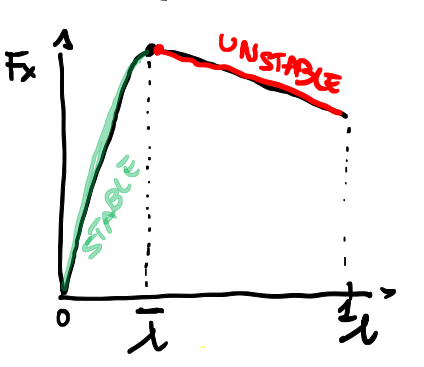
\includegraphics[width=0.5\textwidth]{lectures/2020-04-16/lambda-graph.png}
    \caption*{Relation between $\lambda$ and the breaking force.}
\end{figure}

\begin{figure}[H]
    \centering
    \begin{tikzpicture}[node distance=2.5cm,auto,>=latex']
        \node [int] (abs) {ABS algo};
        \node [sum] (sum) [left of=abs, node distance=2cm] {};
        \node (in) [left of=sum, node distance=2cm] {};
        \node [int] (sys) [right of=abs, node distance=3cm]{System};
        \node [coordinate] (split) [right of=sys, node distance=2cm]{};
        \node (end) [right of=sys, node distance=4cm]{};
        \node [int] (sws) [below of=sys, node distance=1cm]{SW-sensing};

        \draw[->] (in) edge node {$\overline{\lambda}$} (sum);
        \draw[->] (sum) edge node {} (abs);
        \draw[->] (abs) edge node {$u(t)$} (sys);
        \draw[->] (sys) edge node[pos=0.8] {$\lambda$} (end);
        \draw[->] (split) |- node {} (sws);
        \draw[->] (sws) -| node[pos=0.9] {$-$} (sum);
    \end{tikzpicture}
    \caption*{ABS system}
\end{figure}

The problem can be divided into subproblems:
\begin{itemize}
    \item Model of the system
    \item SW-estimation of $\lambda$ ($v$ is not directly measurable, so $\lambda$ cannot be computed)
    \item Design of the ABS control algorithm
\end{itemize}

Why black-box modelling?
The control variable $v$ (the voltage to the actuator) controls a complex systems from the actuator to $\lambda$.
The system can be seen as a chain of components:
\begin{itemize}
    \item Current dynamics and electric motor
    \item Position dynamics of the actuator
    \item Dynamics of the hydraulic circuit of the break system
    \item Tire dynamics
    \item Wheel rotational dynamics
    \item Vehicle full dynamics
\end{itemize}

White box (physical) modelling: write the equations from \emph{first principles}.

Black box modelling: experiment $\rightarrow$ collect data $\rightarrow$ build model.
Using only I/O measured data we can \emph{learn} a mathematical model of the I/O behavior of the system.

\chapter{Black-box non-parametric identification of I/O systems using state-space models}

\begin{figure}[H]
    \centering
    \begin{tikzpicture}[node distance=2.5cm,auto,>=latex']
        \node [int, ellipse] (sys) {system};
        \node (in) [left of=sys, node distance=2cm] {};
        \node (noise) [above of=sys, node distance=1.5cm] {};
        \node (end) [right of=sys, node distance=2cm]{};

        \draw[->] (in) edge node {$u(t)$} (sys);
        \draw[->,dotted] (noise) edge node {$d(t)$ \emph{(not measured disturbance)}} (sys);
        \draw[->] (sys) edge node {$y(t)$} (end);
    \end{tikzpicture}
\end{figure}

\textbf{Measured data}
\begin{align*}
    \left\{u(1), u(2), \ldots, u(N)\right\} &\quad \text{(input)} \\
    \left\{y(1), y(2), \ldots, y(N)\right\} &\quad \text{(output)}
\end{align*}

\begin{remark}[general path of a parametric identification methods]
\end{remark}

\begin{enumerate}
    \item Collect data: $\left\{u(1), u(2), \ldots, u(N)\right\}$, $\left\{y(1), y(2), \ldots, y(N)\right\}$
    \item Select \textbf{a-priori} a class/family of parametric models: $\mathcal{M}(\theta)$
    \item Select \textbf{a-priori} a performance index (it gives an order to the quality of the models)
    \item Optimization step (minimize $J(\theta)$ w.r.t $\theta$): $\hat{\theta}_N = \argmin_\theta J(\theta)$ $\rightarrow$ optimal model $\mathcal{M}(\hat{\theta}_N)$
\end{enumerate}

$J(\theta): \RR^{n_\theta} \rightarrow \RR^+$ (where $n_\theta$ is the order of the model).

$\mathcal{M}(\theta_1)$ is better than $\mathcal{M}(\theta_2)$ if $J(\theta_1) < J(\theta_2)$.

In this chapter we are presenting a totally different system identification approach: \textbf{not parametric}.
\begin{itemize}
    \item No a-priori model-class selection
    \item No performance index definition
    \item No optimization task
\end{itemize}

\section{Representations}

\subsection{Representation \#1: state-space}

\[
\begin{cases}
    x(t+1) = F x(t) + G u(t) & \qquad \text{state equations} \\
    y(t+1) = H x(t) + D u(t) & \qquad \text{output equations}
\end{cases}
\]

Where $F$, $G$, $H$ and $D$ are matricies defined as follows:
\begin{align*}
    F = \begin{bmatrix}
        \\
        n \times n \\
        \text{state matrix} \\ \\
    \end{bmatrix}
    &
    \qquad
    G = \begin{bmatrix}
        \\
        \\
        n \times 1 \\
        \text{input} \\
        \text{matrix} \\ \\
    \end{bmatrix}
    \\ \\
    H = \begin{bmatrix}
        1 \times n \;\;\; \text{output matrix}
    \end{bmatrix}
    &
    \qquad
    D = \begin{bmatrix}
        1 \times 1 \;\;\; \text{i/o matrix}
    \end{bmatrix}
\end{align*}

Assuming 1 input and 1 output, it can be extended for multiple inputs and outputs. Usually $D=0$ for \emph{strictly-proper systems}.

\begin{remark}[S.S representation is not unique]
    $F_1 = TFT^{-1}$, $G_1 = TG$, $H_1 = HT^{-1}$, $D_1 = D$ for any invertible matrix $T$. The system $\{F, G, H, D\}$ is equivalent to $\{F_1, G_1, H_1, D_1\}$.
\end{remark}

\begin{example}
    \[
        \begin{cases}
            x_1(t+1) = \frac{1}{2} x_1(t) + 2u(t) \\
            x_2(t+1) = x_1(t) + 2x_2(t) + u(t) \\
            y(t) = \frac{1}{4}x_1(t) + \frac{1}{2}x_2(t)
        \end{cases}
    \]
    In this case $n=2$, $x(t) = \begin{bmatrix}
        x_1(t) \\
        x_2(t)
    \end{bmatrix}$, one input $u(t)$ and one output $y(t)$.

    \begin{align*}
        F = \begin{bmatrix}
            \frac{1}{2} & 0 \\
            1 & 2
        \end{bmatrix}
        & \qquad
        G = \begin{bmatrix}
            2 \\ 1
        \end{bmatrix}
        \\
        H = \begin{bmatrix}
            \frac{1}{4} & \frac{1}{2}
        \end{bmatrix}
        & \qquad
        D = 0
    \end{align*}
\end{example}

\subsection{Representation \#2: transfer-function}

\[
    W(z) = \frac{B(z)}{A(z)} z^{-k} = \frac{b_0 + b_1z_{-1} + b_2z^{-2} + \ldots + b_pz^{-p}}{a_0 + a_1z^{-1} + a_2z^{-2} + \ldots + a_nz^{-n}} z^{-k}
\]

$W(z)$ is a rational function of the \emph{z} operator: it's a \emph{digital filter}.

It's very easy to move from T.F. representation to a time domain description of the system.

\begin{example}
    \begin{align*}
        & y(t) = \underbrace{\begin{bmatrix}
            \frac{1+\frac{1}{2}z^{-1}}{2+\frac{1}{3}z^{-1}+\frac{1}{4}z^{-2}} z^{-1}
        \end{bmatrix}}_{W(z)} u(t) \\
        & 2y(t) + \frac{1}{3}y(t-1) + \frac{1}{4}y(t-2) = u(t-1) + \frac{1}{2}u(t-2) \\
        & y(t) = \underbrace{-\frac{1}{6}y(t-1) - \frac{1}{8}y(t-2)}_\text{old values of $y(t)$} + \underbrace{\frac{1}{2}u(t-1) + \frac{1}{4}u(t-2)}_\text{old values of input}
    \end{align*}

\end{example}

\begin{remark}[Strictly proper systems]
    Notice that for strictly proper systems the delay $k \ge 1$
\end{remark}
\missingfigure{Graphs about strictly proper systems}

\subsection{Representation \#3: convolution of the input with the Impulse Response (IR)}
The third way to represent a system is through the convolution of the input with the \emph{Impulse Response (IR)}.
\missingfigure{Graphs about convolution}
It can be proven that the input-output relationship from $u(t)$ to $y(t)$ can be written as
\[ y(t) = \omega(0) u(t) + \omega(1) u(t-1) + \omega(2) u(t-2) + \cdots \]
It can be rewritten as follows
\[ y(t) = \sum_{k=0}^{\infty} \omega(k) u(t-k) \]
From this, it is clear that $y(t)$ is the convolution of IR with the input signal.
\missingfigure{Block diagram of system}

\section{Transformation between representations}
\missingfigure{Figure of translation between representations}
\subsection{State Space to Transfer Function}
Consider a strictly proper system with the following state space representation:
\[
\begin{cases}
    x(t+1) = F x(t) + G u(t)\\
    y(t) = H x(t) + \cancelto{0}{D u(t)}\\
\end{cases}
\Rightarrow
\begin{cases}
    x(t+1) = F x(t) + G u(t)\\
    y(t) = H x(t)\\
\end{cases}
\]
From the system we get
\[ z x(t) = F x(t) + G u(t) \Rightarrow x(t) = (zI - F)^{-1} G u(t) \]
\[ \Rightarrow y(t) = H (zI - F)^{-1} G \cdot u(t) \]
Thus, the transfer function is
\[ W(z) = H(zI - F) ^ {-1} G \]

\begin{example}
\begin{align*}
    F = \begin{bmatrix}
        1 & 0\\
        \frac{1}{2} & 2\\
    \end{bmatrix}
    &&
    G = \begin{bmatrix}
        1\\
        1\\
    \end{bmatrix}
    &&
    H = \begin{bmatrix}
        1 & 0\\
    \end{bmatrix}
    &&
    D = 0
\end{align*}
\begin{align*}
W(z) &=
\begin{bmatrix}
    1 & 0\\
\end{bmatrix}
\left( \begin{bmatrix}
    z & 0\\
    0 & z\\
\end{bmatrix}
-
\begin{bmatrix}
    1 & 0 \\
    \frac{1}{2} & 2\\
\end{bmatrix}\right)^{-1}
\begin{bmatrix}
    1\\
    1\\
\end{bmatrix}
= \begin{bmatrix}
    1 & 0\\
\end{bmatrix}
\begin{bmatrix}
    z-1 & 0\\
    -\frac{1}{2} & z-2\\
\end{bmatrix}^{-1}
\begin{bmatrix}
    1\\
    1\\
\end{bmatrix}\\
&= \begin{bmatrix}
    1 & 0\\
\end{bmatrix}
\frac{1}{(z-1)(z-2)}
\begin{bmatrix}
    z-2 & 0\\
    \frac{1}{2} & z-1\\
\end{bmatrix}
\begin{bmatrix}
    1\\
    1\\
\end{bmatrix}
=
\frac{1}{(z-1)(z-2)}
\begin{bmatrix}
    z-2 & 0\\
\end{bmatrix}
\begin{bmatrix}
    1\\
    1\\
\end{bmatrix}\\
&=
\frac{\cancel{z-2}}{(z-1)\cancel{(z-2)}} = \frac{1}{z-1} = \frac{1}{1-z^{-1}} z^{-1}
\end{align*}
Notice that in this case we only have one pole, but the system is of order two; this comes from the fact that part of the system is non observable.

\end{example}

\subsection{Transfer Function to State Space}
This conversion is not very used in practice and it is called the \emph{realization} of a transfer function into a state space model.

Note that the state space representation is not unique, so from a single transfer function we can get infinite different equivalent state space models.

\subsubsection{Control realization}

We assume that the system is strictly proper and that the denominator is monic.
\[ W(z) = \frac{b_0 z^{n-1} + b_1 z^{n-2} + \dots + b_{n-1}}{z^n + a_1 z^{n-1} + a_2 z^{n-2} + \dots + a_n} \]

The formula for the control realization of $W(z)$ is
\begin{align*}
    F = \begin{bmatrix}
        0 & 1 & 0 & \cdots & 0\\
        0& 0 & 1 & \ddots & \vdots \\
        \vdots & \vdots & \ddots & \ddots & 0\\
        0 & 0 & \cdots & 0 & 1\\
        -a_n & -a_{n-1} & \multicolumn{2}{c}{\cdots} & -a_1\\
    \end{bmatrix}
    &&
    G = \begin{bmatrix}
        0\\
        0\\
        0\\
        \vdots\\
        1\\
    \end{bmatrix}
    &&
    H = \begin{bmatrix}
        b_{n-1} & b_{n-2} & \cdots & b_0\\
    \end{bmatrix}
    &&
    D = 0
\end{align*}
\begin{example}
    Consider the transfer function $W(z)$
    \[ W(z) = \frac{2z^2 + \frac{1}{2}z + \frac{1}{4}}{z^3 + \frac{1}{4}z^2 + \frac{1}{3}z + \frac{1}{5}} \]
    The control realization is
    \begin{align*}
        F = \begin{bmatrix}
            0 & 1 & 0\\
            0 & 0 & 1\\
            -\frac{1}{5} & -\frac{1}{3} & -\frac{1 }{4}\\
        \end{bmatrix}
        &&
        G = \begin{bmatrix}
            0\\
            0\\
            1\\
        \end{bmatrix}
        &&
        H = \begin{bmatrix}
            \frac{1}{4} & \frac{1}{2} & 2\\
        \end{bmatrix}
        &&
        D = 0
    \end{align*}
\end{example}

\subsection{Transfer Function to Impulse Response}
To get the IR from a transfer function $W(z)$ is sufficient to make the $\infty$-long division between the numerator and denominator of $W(z)$
\begin{example}
    Consider the transfer function
    \[ W(z) = \frac{1}{z-\frac{1}{2}} = \frac{z^{-1}}{1-\frac{1}{2}z^{-1}}
        = 0 z^{-0} + 1 z^{-1} + \frac{1}{2}z^{-2} + \frac{1}{4}z^{-3} + \cdots \]
    Thus the IR is $\omega(0) = 0$, $\omega(1) = 1$, $\omega(2) = \frac{1}{2}$, $\omega(3) = \frac{1}{4}$, $\dots$

    In this case there is also a quicker way
    \[ y(t) = \frac{z^{-1}}{1-\frac{1}{2}z^{-1}} u(t) = \left( z^{-1} \frac{1}{1-\frac{1}{2}z^{-1}} \right) u(t) \]
    Remembering that for geometric series we have \[ \sum_{k = 0}^{\infty} a^k = \frac{1}{1-a} \text{ if } |a| < 1 \]
    We can rewrite $y(t)$ as follows
    \[ y(t) = \left( z^{-1} \sum_{k=0}^{\infty} \left( \frac{1}{2} z^{-1} \right)^{k} \right) u(t) = \left( 0 + 1 z^{-1} + \frac{1}{2}z^{-2} + \frac{1}{4}z^{-3} + \cdots \right) u(t) \]
\end{example}

\subsection{Impulse Response to Transfer Function}
\begin{definition}
    Given a discrete-time signal $s(t)$ such that $\forall t < 0: s(t) = 0$, its \emph{Z-Transform} is defined as
    \[ \mathcal{Z} \left( s(t) \right) = \sum_{t = 0}^{\infty} s(t) z^{-t} \]
\end{definition}
Given this, it can be proven that
\[ W(z) = \mathcal{Z}\left( \omega(t) \right) = \sum_{t = 0}^{\infty} \omega(t) z^{-t} \]
This means that the transfer function of a system is the $\mathcal{Z}$-transform of a special signal, that is the impulse response of the system.

\begin{remark}
    This formula cannot be used in practice to transform an IR representation to a TF representation.
    This is because we need infinite points of the impulse response, and the impulse response must be noise-free.
    Thus, this transformation is only theoretical.
\end{remark}

\subsection{State Space to Impulse Reponse}
Consider the following state space model, with initial conditions $x(0) = 0$ and $y(0) = 0$
\[
    \begin{cases}
        x(t+1) = F x(t) + G u(t)\\
        y(t) = H x(t)\\
    \end{cases}
\]
We have that
\begin{align*}
    x(1) &= \cancelto{0}{F x(0)} + G u(0) = G u(0)\\
    y(1) &= H x(1) = H G u(0)\\
\end{align*}
\begin{align*}
    x(2) &= F x(1) + G u(1) = F G u(0) + G u(1)\\
    y(2) &= H x(2) = H F G u(0) + H G u(1)\\
\end{align*}
\begin{align*}
    x(3) &= F x(2) + G u(2) = F^2 G u(0) + F G u(1) + G u(2)\\
    y(3) &= H x(3) = H F^2 G u(0) + H F G u(1) + H G u(2)\\
\end{align*}
This can be generalized to
\[ y(t) = 0 u(t) + H G u(t-1) + H F G u(t-2) + H F^2 G u(t-3) + \cdots \]
Thus, the impulse response is
\[
    \omega(t) =
    \begin{cases}
        0 \text{ if } t = 0\\
        H F^{t-1} G \text{ if } t > 0\\
    \end{cases}
\]

\subsection{Summary of transformations}
Notice that the IR representation is very easy to obtain experimentally, since we only need to measure the system response to the impulse signal.
However, given the IR representation, it is difficult to get to the other representations, since the transformation between from IR to TF is only theoretical.
Moving from the IR to the SS representation is the key task of the \emph{Subspace-based State Space System Identification}, also known as \emph{4SID methods}.

\section{Subspace-based State Space System Identification (4SID)}
The original 4SID method starts from the measurement of the system output in a very simple experiment, that is the \emph{impulse experiment}.
\missingfigure{Impulse response}
The fundamental idea is that it is very simple to make this experiment, that is to measure the output of system given an impulse signal as the input.
The real problem is to identify a model $\left\{ \hat{F}, \hat{G}, \hat{H} \right\}$ starting from $\left\{ \omega(0), \omega(1), \omega(2), \cdots \right\}$.

We will see the solution of this problem in two steps:
\begin{enumerate}
    \item IR measurement is assumed to be noise-free.
    This is easier with respect to the original problem, but it is also not realistic.
    \item IR is measured with noise
    \[ \widetilde{\omega}(t) = \omega(t) + \eta(t) \quad t = 0, 1,\dots, N \]
    \begin{itemize}
        \item $\widetilde{\omega}(t)$ is the measured noisy IR
        \item $\omega(t)$ is the ``true'' noise-free IR
        \item $\eta(t)$ is the measurement noise (e.g. WN)
    \end{itemize}
\end{enumerate}
\begin{remark}
    We will see in detail only 4SID when the experiment is an impulse-experiment, which is the first and original version of 4SID.
    However 4SID can be extended to any generic input signal $\left\{ u(1), u(2), \cdots, u(N) \right\}$ that is sufficiently exciting.
\end{remark}
\begin{remark}[Unstable system]
    In case of an unstable system the measurements must be collected in a closed-loop experiment.
    Indeed, if the experiment was open-loop, the experiment would be unfeasible.
    \missingfigure{Unstable system}
    \missingfigure{Closed loop system}
\end{remark}
\newlecture{Sergio Savaresi}{21/04/2020}

\begin{figure}[H]
    \centering
    \begin{tikzpicture}[node distance=2.5cm,auto,>=latex']
        \node (n1) {\#1};
        \node (n2) [below of=n1, xshift=-1.8cm] {\#2};
        \node (n3) [below of=n1, xshift= 1.8cm] {\#3};

        \draw[->] (n1) edge[bend right] (n2);
        \draw[->] (n2) edge[bend right] (n3);
        \draw[->] (n1) edge[bend left] (n3);
        \draw[->, dashed] (n2) edge[bend right=20] (n1);
        \draw[->, dotted] (n3) edge[bend right=20] (n2);
        \draw[->, dashed, red] (n3) edge[bend left=20] node {?} (n1);
    \end{tikzpicture}
\end{figure}

\section{Fundamental concepts of observability and controllability}

\[
    \begin{cases}
        x(t+1) = Fx(t) + Gu(t) \\
        y(t) = Hx(t)
    \end{cases}
\]

\subsection{Fully Observable}
The system is fully observable (from the output) if and only if the observability matrix is full rank:
\[
    O = \begin{bmatrix}
        H \\
        HF \\
        \vdots \\
        HF^{n-1}
    \end{bmatrix}
    \qquad
    \rank O = n
\]

\subsection{Fully Controllable}
The system is fully controllable (from the input) if and only if the controllability matrix is full rank:
\[
    R = \begin{bmatrix}
        G & FG & \cdots & F^{n-1}G
    \end{bmatrix}
    \qquad
    \rank R = n
\]

$R$ is also called \emph{reachability} matrix.

\begin{remark}
    \begin{description}
        \item[Observability] we can observe the state from the output sensors.
        \item[Controllability] we can control/move/influence the state using the input signal.
    \end{description}
\end{remark}

\begin{example}
    \begin{align*}
        \begin{cases}
            x_1(t+1) = \frac{1}{2} x_1(t) + u(t) \\
            x_2(t+1) = \frac{1}{3}x_2(t) \\
            y(t) = \frac{1}{4}x_1(t)
        \end{cases}
        \qquad
        F = \begin{bmatrix}
            \frac{1}{2} & 0 \\
            0 & \frac{1}{3}
        \end{bmatrix}
        \qquad
        H = \begin{bmatrix}
            \frac{1}{4} & 0
        \end{bmatrix}
        \qquad
        G = \begin{bmatrix}
            1 \\
            0
        \end{bmatrix}
    \end{align*}

    \[
        O = \begin{bmatrix}
            H \\
            HF
        \end{bmatrix} = \begin{bmatrix}
            \frac{1}{4} & 0 \\
            \frac{1}{8} & 0
        \end{bmatrix}
        \qquad
        \rank O = 1 < n = 2
        \quad\implies\quad \text{not fully observable}
    \]

    \[
        R = \begin{bmatrix}
            G & FG
        \end{bmatrix} = \begin{bmatrix}
            0 & 0 \\
            1 & \frac{1}{3}
        \end{bmatrix}
        \qquad
        \rank R = 1 < n = 2
        \quad\implies\quad \text{not fully controllable}
    \]
\end{example}

\begin{remark}[4 sub-systems]
    Each system can be internally seen as 4 sub-systems as follows:

    \begin{figure}[H]
        \centering
        \begin{tikzpicture}[node distance=1.5cm,auto,>=latex']
            \node[int, align=center] (noc) {NO\\C};
            \node[int, align=center, below of=noc] (onc) {O\\NC};
            \node[int, align=center, below of=onc] (oc) {O\\C};
            \node[int, align=center, below of=oc] (nonc) {NO\\NC};

            \node at (-5cm,-1.5cm) (u) {$u$};
            \node[coordinate] at (-3cm,-1.5cm) (input) {};
            \node at (5cm,-2.5cm) (y) {$y$};
            \node[coordinate] at (3cm,-2.5cm) (output) {};
            \node[right of=noc] (noc_out) {};
            \node[right of=nonc] (nonc_out) {};
            \node[left of=onc] (onc_in) {};

            \draw[-{Rays[n=4]}] (noc) -- (noc_out);
            \draw[-{Rays[n=4]}] (nonc) -- (nonc_out);
            \draw[{Rays[n=4]}-] (onc_in) -- (onc);
            \draw (input) edge[->, bend left=10] (noc);
            \draw[line width=0.5mm] (input) edge[->, bend right=10] (oc);
            \draw[line width=0.5mm] (u) edge (input);
            \draw (onc) edge[bend left=10] (output);
            \draw[line width=0.5mm] (oc) edge[bend right=10] (output);
            \draw[line width=0.5mm] (output) edge[->] (y);

            \draw[draw=black] (-4cm,-5.5cm) rectangle ++(8cm,6.5cm);
        \end{tikzpicture}
    \end{figure}

    Which externally is equivalent to a systems like this:
    \begin{figure}[H]
        \centering
        \begin{tikzpicture}[node distance=1.5cm,auto,>=latex']
            \node[int, align=center] (oc) {O\\C};
            \node[left of=oc] (in) {$u$};
            \node[right of=oc] (out) {$y$};

            \draw[->] (in) -- (oc);
            \draw[->] (oc) -- (out);
        \end{tikzpicture}
    \end{figure}
\end{remark}

\section{Hankel matrix of order n}

Starting from $IR = \{\omega(1), \omega(2), \ldots, \omega(N)\}$ we can build the Hankel matrix of order $n$.

\[
    H_n = \begin{bmatrix}
        \omega(1) & \omega(2) & \omega(3) & \cdots & \omega(n) \\
        \omega(2) & \omega(3) & \omega(4) & \cdots & \omega(n+1) \\
        \omega(3) & \omega(4) & \omega(5) & \cdots & \omega(n+2) \\
        \vdots    & \vdots    & \vdots    & \ddots & \vdots \\
        \omega(n) & \omega(n+1) & \omega(n+2) & \ldots & \omega(2n-1)
    \end{bmatrix}
\]

\textbf{Note} that we need IR up to time $2n-1$.

\textbf{Note} it starts from $\omega(1)$ and not $\omega(0)$.

\textbf{Note} the anti-diagonals all have the same element repeated.

We know that $\omega(t) = \begin{cases}
    0 &\quad \text{if } t = 0 \\
    HF^{t-1}G &\quad \text{if } t > 0
\end{cases}$ therefore $H_n$ can be rewritten as

\[
    H_n = \begin{bmatrix}
        HG     & HFG    & HF^2G  & \cdots & HF^{n-1}G \\
        \vdots & \ddots &        &        & \vdots \\
        \vdots &        & \ddots &        & \vdots \\
        \vdots &        &        & \ddots & \vdots \\
        HF^{n-1}G & \cdots & \cdots & \cdots & HF^{2n-2}G
    \end{bmatrix} = \begin{bmatrix}
        H \\
        HF \\
        \vdots \\
        HF^{n-1}
    \end{bmatrix} \cdot \begin{bmatrix}
        G & FG & \cdots & F^{n-1}G
    \end{bmatrix} = O \cdot R
\]

Where $O$ is the observability matrix and $R$ is the reachability matrix.

\section{Algorithm to obtain $\hat{F}$, $\hat{G}$, $\hat{H}$ from a noise-free measured IR}

\paragraph{Step 1} Build the Hankel matrix in increasing order and each time compute the rank of the matrix.

\[
    H_1 = \begin{bmatrix}
        \omega(1)
    \end{bmatrix}
    \qquad
    H_2 = \begin{bmatrix}
        \omega(1) & \omega(2) \\
        \omega(2) & \omega(3)
    \end{bmatrix}
    \qquad
    H_3 = \ldots
    \qquad
    \cdots
    \qquad
    H_n = \ldots
\]

Suppose that $\rank H_n = n$ and $\rank H_{n+1} = n$.
With this procedure we know the order of the system.

\paragraph{Step 2} Take $H_{n+1}$ (with $\rank H_{n+1} = n$), factorize it in two rectangular matrices of size $(n+1) \times n$ and $n \times (n+1)$.

\[
    H_{n+1} = \begin{bmatrix}
        \text{extended} \\
        \text{observability} \\
        \text{matrix} \\
        O_{n+1}
    \end{bmatrix} \cdot \begin{bmatrix}
        \text{extended} \\
        \text{controllability} \\
        \text{matrix} \\
        R_{n+1}
    \end{bmatrix}
\]

Where $O_{n+1} = \begin{bmatrix}
    H \\ HF \\ \vdots \\ HF^n
\end{bmatrix}$ of size $(n+1)\times n$ and $R_{n+1} = \begin{bmatrix}
    G & FG & \cdots & F^nG
\end{bmatrix}$ of size $n\times (n+1)$.

\paragraph{Step 3} $H$, $F$, $G$ estimation.

Using $O_{n+1}$ and $R_{n+1}$ we can easily find:
\begin{align*}
    \hat{G} = R_{n+1}(\texttt{:;1}) & \quad\text{first column} \\
    \hat{H} = O_{n+1}(\texttt{1;:}) & \quad\text{first row} \\
\end{align*}

Define $O_1$ as $O_{n+1}$ without the last row, and $O_2$ as $O_{n+1}$ without the first row.
$O_1$ and $O_2$ are $n\times n$ matrices.
This is called \emph{shift-invariance} property.

\textbf{Note} that $O_1$ is invertible since it's an observability matrix and the subsystem is fully observable.
Moreover $O_1F = O_2$, so $\hat{F} = O_1^{-1}O_2$.

In conclusion in a simple and constructive way we have estimated a State Space model of the system $\{\hat{H}, \hat{G}, \hat{F}\}$ starting from measured IR, using only $2n+1$ samples of IR.

\begin{remark}
    If the measurement is noisy all this process is useless.
\end{remark}

\section{Real problem}

The measurements of IR are noisy: $\tilde{\omega}(t) = \omega(t) + \eta(t)$.

\begin{figure}[H]
    \begin{minipage}[t]{0.5\textwidth}
        \centering
        \begin{tikzpicture}[node distance=2.5cm,auto,>=latex']
            \draw[->] (-0.5,0) -- (3,0) node[right] {$t$};
            \draw[->] (0,-1) -- (0,2) node[left] {$u(t)$};
            \draw[domain=-0.3:0,smooth,variable=\x,red] plot ({\x},{0});
            \draw[domain=0:0.2,smooth,variable=\x,red] plot ({\x},{1.5});
            \draw[domain=0.2:2.5,smooth,variable=\x,red] plot ({\x},{0});
        \end{tikzpicture}
        \caption*{Input}
    \end{minipage}
    \begin{minipage}[t]{0.5\textwidth}
        \centering
        \begin{tikzpicture}[node distance=2.5cm,auto,>=latex']
            \draw[->] (-0.5,0) -- (3,0) node[right] {$t$};
            \draw[->] (0,-1) -- (0,2) node[left] {$y(t)$};
            \draw[domain=0:2.5,smooth,variable=\x,red] plot ({\x},{cos(\x*180/3.14*5)*e^(-\x)});
            \draw[samples=100, domain=0:2.5,smooth,variable=\x,blue] plot ({\x},{cos(\x*180/3.14*5)*e^(-\x)+rand/4});
        \end{tikzpicture}
        \caption*{Output}
    \end{minipage}
\end{figure}

\section{4SID procedure (with noise)}

\paragraph{Step 1} Build the Hankel matrix from data using ``one-shot'' all the available $N$ data points.

\[
    \tilde{H}_{qd} = \begin{bmatrix}
        \tilde{\omega}(1) & \tilde{\omega}(2) & \cdots & \tilde{\omega}(d) \\
        \tilde{\omega}(2) & \tilde{\omega}(3) & \cdots & \tilde{\omega}(d+1) \\
        \vdots            & \vdots            & \ddots & \vdots \\
        \tilde{\omega}(q) & \tilde{\omega}(q+1) & \cdots & \tilde{\omega}(q+d-1) \\
    \end{bmatrix}
\]

$\tilde{H}_{qd}$ is a $q\times d$ matrix. \textbf{Note} that $q+d-1$ must equal to $N$ so that we use all the data set.

\begin{remark}[Choice of $q$ and $d$]
    Hypothesis: $q<d$ so that $q+d-1=N$, so $q=N+1-d$.
    \begin{figure}[H]
        \centering
        \begin{tikzpicture}[node distance=2.5cm,auto,>=latex']
            \draw[->] (-0.5,0) -- (3,0) node[right] {$d$};
            \draw[->] (0,-0.5) -- (0,3) node[left] {$q$};
            \draw[domain=0.3:2.7,smooth,variable=\x,black] plot ({\x},{3-\x});
            \draw[line width=0.6mm,domain=1.5:1.8,smooth,variable=\x,green] plot ({\x},{3-\x});
            \draw[line width=0.6mm,domain=2.3:2.7,smooth,variable=\x,blue] plot ({\x},{3-\x});
            \draw[dotted] (0,0) -- (1.5,1.5);

            \node at (2.3,1.5) {$q \approx d$};
            \node at (3.1,0.7) {$q \ll d$};

            \node[below] at (0.3,0) {$1$};
            \node[below] at (2.7,0) {$N$};
            \node[left] at (0,0.3) {$1$};
            \node[left] at (0,2.7) {$N$};
        \end{tikzpicture}
    \end{figure}

    If $q \approx d$ the method has better accuracy.
    If $q \ll d$ it's computationally less intensive.

    If $0.6d < q < d$ we get to a good enough result.
\end{remark}

\newlecture{Sergio Savaresi}{21/04/2020}

\paragraph{Step 2} Singular Value Decomposition (SVD) of $\tilde{H}_{qd}$

\[
    \underbrace{\tilde{H}_{qd}}_{q\times d} = \underbrace{\tilde{U}}_{q\times q} \underbrace{\tilde{S}}_{q\times d} \underbrace{\tilde{V}^T}_{d\times d}
\]

$\tilde{U}$ and $\tilde{V}$ are unitary matrices. A matrix $M$ is unitary if:
\begin{itemize}
    \item $\det M = 1$ (so it's invertible)
    \item $M^{-1} = M^T$
\end{itemize}

\[
    \tilde{S} = \begin{bmatrix}
        \sigma_1 & & & & &\\
        & \sigma_2 & & & &\\
        & & \ddots & & &\\
        & &  & \sigma_d & &\\
    \end{bmatrix}
\]

Where $\sigma_1$, $\sigma_2$, $\ldots$, $\sigma_q$ are the singular values of $\tilde{H}_{qd}$.
Those are real, positive numbers, sorted in decreasing order ($\sigma_1 \ge \sigma_2 \ge \cdots \ge \sigma_q$).

\begin{remark}
    The singular values of a rectangular matrix are a \emph{sort of} eigenvalues of a square matrix.\\
    SVD is a \emph{sort of} diagonalization of a rectangular matrix.
\end{remark}

\begin{remark}
    For a square matrix, $\text{eig}(A) = \text{roots}(\det(A-\lambda I))$. If $M$ is rectangular, $SV(M) = \sqrt{\text{eig}(MM^T)}$ (for non zero eigenvalues).
\end{remark}

\begin{remark}[How to compute SVD]
    The optimal numerical computation is not trivial. Use \texttt{svd(M)} in Matlab.

    Theoretical method for SVD computation is to make 2 diagonalization steps:
    \[
        \underbrace{\tilde{H}_{qd} \tilde{H}_{qd}^T}_{q\times q} = \tilde{U}\tilde{S}\tilde{S}^T\tilde{U}^T
    \]
    \[
        \underbrace{\tilde{H}_{qd}^T \tilde{H}_{qd}}_{d\times d} = \tilde{V}\tilde{S}^T\tilde{S}\tilde{V}^T
    \]
\end{remark}

\paragraph{Step 3} Plot the singular values and cut-off the 3 matrices.

\begin{figure}[H]
    \begin{minipage}[t]{0.5\textwidth}
        \centering
        \begin{tikzpicture}[node distance=2.5cm,auto,>=latex']
            \draw[->] (0,0) -- (5,0) node[right] {$i$};
            \draw[->] (0,0) -- (0,2) node[left] {$\sigma_i$};
            \node at (0.5,1.8) {\textbullet};
            \node at (1.0,1.3) {\textbullet};
            \node at (1.5,1.0) {\textbullet};
            \node at (2.0,0.9) {\textbullet};
            \node at (2.5,0.8) {\textbullet};
            \node at (3.0,0.2) {\textbullet};
            \node at (3.5,0.2) {\textbullet};
            \node at (4.0,0.2) {\textbullet};
            \node at (4.5,0.2) {\textbullet};
            \draw (2.5,-0.1) -- (2.5,0.1);
            \node at (2.5,-0.4) {$n$};

            \draw[decoration={brace}, decorate] (0.5,2) node {} -- (2.5,1);
            \node at (2.5,1.8) {signal SV};

            \draw[decoration={brace}, decorate] (3,0.4) node {} -- (4.5,0.4);
            \node at (3.75,0.8) {noise SV};
        \end{tikzpicture}
        \caption*{Ideal case}
    \end{minipage}
    \begin{minipage}[t]{0.5\textwidth}
        \centering
        \begin{tikzpicture}[node distance=2.5cm,auto,>=latex']
            \draw[->] (0,0) -- (5,0) node[right] {$i$};
            \draw[->] (0,0) -- (0,2) node[left] {$\sigma_i$};
            \node at (0.5,1.8) {\textbullet};
            \node at (1.0,1.3) {\textbullet};
            \node at (1.5,1.0) {\textbullet};
            \node at (2.0,0.8) {\textbullet};
            \node at (2.5,0.6) {\textbullet};
            \node at (3.0,0.4) {\textbullet};
            \node at (3.5,0.3) {\textbullet};
            \node at (4.0,0.2) {\textbullet};
            \node at (4.5,0.2) {\textbullet};
            \draw (2,-0.1) rectangle ++(1,0.2);
            \node at (2.5,-0.4) {$n$};

            \draw[decoration={brace}, decorate] (2,1) node {} -- (3,1);
            \node at (2.5,1.4) {transition};
        \end{tikzpicture}
        \caption*{Real case}
    \end{minipage}
\end{figure}

In the ideal case there is a perfect/clear separation between the signal and the noise S.V. (a jump).
The index of the jump is $n$, that is the order of the system.

In the real case there is no clear distinction between signal and noise singular values, the order of the system can assume values in an interval.
With some empirical test we can select a good compromise between complexity, precision and overfitting (see \emph{cross-validation}).

After the decision on the value of $n$ we split $\tilde{U}$, $\tilde{S}$ and $\tilde{V}^T$:

\begin{figure}[H]
    \centering
    \begin{tikzpicture}
        \tikzset{BarreStyle/.style = {opacity=.3,line width=4 mm,color=blue}}
        \node (H) {$\tilde{H}_{qd} =$};
        \matrix (U) [right of=H, node distance=2cm,matrix of math nodes, nodes in empty cells,left delimiter={[},right delimiter={]},text depth=0ex,text height=1ex,text width=1ex]
        {
            & & & & \\
            & & & & \\
            \hat{U} & & \tilde{U} & & \\
            & & & & \\
            & & & & \\
        };
        \matrix (S) [right of=U,node distance=3cm,matrix of math nodes, nodes in empty cells,left delimiter={[},right delimiter={]},text depth=0ex,text height=1ex,text width=1ex]
        {
            \hat{S} & & & & \\
            & & & & \\
            & & \tilde{S} & & \\
            & & & & \\
            & & & & \\
        };
        \matrix (V) [right of=S,node distance=3cm,matrix of math nodes, nodes in empty cells,left delimiter={[},right delimiter={]},text depth=0ex,text height=1ex,text width=1ex]
        {
            & & \hat{V}^T & & \\
            & & & & \\
            & & \tilde{V}^T & & \\
            & & & & \\
            & & & & \\
        };

        \draw[decoration={brace}, decorate] (1,1.2) node {} -- (1.5,1.2);
        \node at (1.25,1.5) {$q\times n$};
        \draw[decoration={brace}, decorate] (4,1.2) node {} -- (4.5,1.2);
        \node at (4.25,1.5) {$n\times n$};
        \draw[decoration={brace}, decorate] (7,1.2) node {} -- (9,1.2);
        \node at (8,1.5) {$n\times d$};

        \draw [BarreStyle] (U-1-1.north) to (U-5-1.south);
        \draw [BarreStyle] (S-1-1.west) to (S-1-1.east);
        \draw [BarreStyle] (V-1-1.west) to (V-1-5.east);
    \end{tikzpicture}
\end{figure}


\[
    \tilde{H}_{qd} = \underbrace{\hat{U} \hat{S} \hat{V}^T}_{\hat{H}_{qd}} + H_{res,qd} \qquad \rank \tilde{H}_{qd} = q \quad \rank \hat{H}_{qd} = n \quad \rank H_{res,qd} = q
\]

From $\tilde{H}_{qd}$ to $\hat{H}_{qd}$ the rank is hugely reduced.

\paragraph{Step 4} Estimation of $\hat{F}$, $\hat{G}$ and $\hat{H}$ using the cleaned matrix $\hat{H}_{qd}$

\[
    \hat{H}_{qd} = \hat{U} \hat{S} \hat{V}^T = \hat{U} \hat{S}^{\frac{1}{2}} \hat{S}^{\frac{1}{2}} \hat{V}^T
\]

Where $\hat{S}^{\frac{1}{2}}$ is the matrix with elements the square roots of the elements of $\hat{S}$.

\[
    \hat{O} = \hat{U} \hat{S}^{\frac{1}{2}} \qquad \hat{R} = \hat{S}^{\frac{1}{2}} \hat{V}^T \qquad \implies \qquad \hat{H}_{qd} = \hat{O} \hat{R}
\]

We can view $\hat{O}$ as the extended observability matrix and the $\hat{R}$ the extended reachability matrix of the system. We can estimate $\hat{H}$ with the first row of $\hat{O}$ and $\hat{G}$ with the first column of $\hat{R}$.

What about the estimation of $\hat{F}$?
Consider for example $\hat{O}$ and use the \emph{shift-invariance} property.
Define $\hat{O}_1$ as $\hat{O}$ without the last row, and $\hat{O}_2$ as $\hat{O}$ without the first row.

Therefore $\hat{O}_1\cdot \hat{F} = \hat{O}_2$, but $\hat{O}_1$ is not a square matrix so it's not invertible.
In this case we can use the approximate \emph{least-square} solution of this linear system.

Consider a generic system $Ax = B$ with dimension  $(h\times n) \cdot (n \times 1) = (h \times 1)$, we have 3 different cases:
\begin{enumerate}
    \item $h < n$. We have less equations than variables, the system is \emph{under determined} and we have infinite solutions.
    \item $h = n$, we have one and only one solution if $A$ is invertible.
    \item $h > n$, we have more equations than variables, the system is \emph{over determined} and it's impossible (no solutions).
\end{enumerate}

In the third case we can use an approximate solution using the least-squares method, which for a generic system is as follows:
\begin{align*}
    Ax &= B \\
    A^TAx &= A^TB \implies \hat{X} = \underbrace{(A^TA)^{-1}A^T}_{A^+} B
\end{align*}

$A^+$ is called \emph{pseudo-inverse}, which is ``surrogate inverse'' when $A$ is rectangular.

Using the pseudo-inverse matrix:
\begin{align*}
    \hat{O}_1\hat{F} = \hat{O}_2 &&
    \hat{O}_1^T\hat{O}_1\hat{F} = \hat{O}_1^T\hat{O}_2 &&
    \hat{F} = \left(\hat{O}_1^T\hat{O}_1\right)^{-1} \hat{O}_1^T\hat{O}_2
\end{align*}


\paragraph{Conclusion} Starting from a noisy I.R. $\{\widetilde{\omega}(1), \widetilde{\omega}(2), \ldots, \widetilde{\omega}(N)\}$ we have estimated a model $\{\hat{F}, \hat{G}, \hat{H}\}$ in a non parametric and constructive way.

\begin{remark}
    This method can be extended also to the case where the input signal is generic (i.e. not an impulse).
\end{remark}

\begin{remark}[Optimality of 4SID]
    The method is optimal in the sense that it makes the best possible rank reduction of $\tilde{H}_{qd}$.
\end{remark}

\begin{example}[Rank reduction]
    In general there are infinite ways to make a rank reduction.
    \[
        \underbrace{\begin{bmatrix}
            2 & 5 & 3 & 6 & 5 \\
            5 & 3 & 6 & 5 & 7 \\
            3 & 6 & 5 & 7 & 1
        \end{bmatrix}}_{\rank = 3}
        =
        \underbrace{\begin{bmatrix}
            1 & 0 & 0 & 0 & 0 \\
            0 & 1 & 0 & 0 & 0 \\
            0 & 0 & 0 & 0 & 0
        \end{bmatrix}}_{\rank = 2}
        +
        \begin{bmatrix}
            1 & 5 & 3 & 6 & 5 \\
            5 & 2 & 6 & 5 & 7 \\
            3 & 6 & 5 & 7 & 1
        \end{bmatrix}
    \]
    It's not the optimal rank reduction matrix, but it factors out a matrix with lower rank.
\end{example}

Our goal is to obtain the desired rank reduction by discarding the minimum amount of information contained in the original matrix.
SVD makes exactly this: $\tilde{H}_{res,qd}$ is the minimum possible (in the sense of the \emph{Frobenius norm}).
\[
    \left|\tilde{H}_{res,qd}\right|_F = \sqrt{\sum_{ij} \left(\tilde{H}_{res,qd}^{(ij)} \right)^2}
\]

\begin{remark}
    4SID is a constructive method that can be implemented in a fully-automatic way, except for these steps:
    \begin{itemize}
        \item $q$ and $d$ selection (not critical)
        \item Choice of $n$ (typically supervised by the designer). It can be made automatic using a cross-validation method.
    \end{itemize}
\end{remark}

\begin{remark}
    SVD was an historical turning point in machine learning algorithms because it allows:
    \begin{itemize}
        \item Very efficient compression of information.
        \item Very efficient separation of \emph{important} information from noise.
    \end{itemize}
\end{remark}

\newlecture{Sergio Savaresi}{23/04/2020}

\begin{exercise}[similar to an exam exercise]
    Consider the following S.S. model
    \[
    F = \begin{bmatrix}
        \frac{1}{2} & 0 \\
        1   & \frac{1}{4}
    \end{bmatrix}
    \qquad
    G = \begin{bmatrix}
        1 \\ 0
    \end{bmatrix}
    \qquad
    H = \begin{bmatrix}
        0 & 1
    \end{bmatrix}
    \qquad
    D = 0
    \]
    The system has grade $n=2$ and is single-input single-output.

    \paragraph{Question} Write the time domain equations of the system in the state space representation.
    \begin{align*}
        x_1(t+1) &= \frac{1}{2}x_1(t) + u(t) \\
        x_2(t+1) &= x_1(t) + \frac{1}{4}x_2(t) \\
        y(t) &= x_2(t)
    \end{align*}

    \paragraph{Question} Write the block scheme of the S.S. representation of the system.
    \begin{figure}[H]
        \centering
        \begin{tikzpicture}[node distance=2cm,auto,>=latex']
            \node [int] (in1) {$1$};
            \node [left of=in1] (u) {$u(t)$};
            \node [sum, right of=in1, node distance=1.5cm] (sum1) {};
            \node [int, right of=sum1, node distance=2.5cm] (n1) {$z^{-1}$};
            \node [int, below of=n1, node distance=1.5cm] (fb1) {$\frac{1}{2}$};
            \node [coordinate, right of=n1] (exit1) {};
            \node [int, below of=fb1, node distance=1.5cm] (in2) {$1$};
            \node [int, below of=in2, node distance=1.5cm] (n2) {$z^{-1}$};
            \node [sum, left of=n2, node distance=2.5cm] (sum2) {};
            \node [coordinate, right of=n2] (exit2) {};
            \node [int, below of=n2, node distance=1.5cm] (fb2) {$\frac{1}{4}$};
            \node [int, right of=exit2, node distance=1.5cm] (out2) {$1$};
            \node [right of=out2, node distance=1.5cm] (y) {$y(t)$};

            \draw[->] (u) -- (in1);
            \draw[->] (in1) -- (sum1);
            \draw[->] (sum1) edge node {$x_1(t+1)$} (n1);
            \draw (n1) edge node {$x_1(t)$} (exit1);
            \draw[->] (exit1) |- (fb1);
            \draw[->] (exit1) |- (in2);
            \draw[->] (fb1) -| (sum1);
            \draw[->] (in2) -| (sum2);
            \draw[->] (sum2) edge node {$x_2(t+1)$} (n2);
            \draw (n2) edge node {$x_2(t)$} (exit2);
            \draw[->] (exit2) |- (fb2);
            \draw[->] (fb2) -| (sum2);
            \draw[->] (exit2) -- (out2);
            \draw[->] (out2) -- (y);
        \end{tikzpicture}
    \end{figure}


    By visual inspection the system is fully observable and fully controllable.

    \paragraph{Question} Make a formal verification that the system is fully observable and controllable.
    \[
        O = \begin{bmatrix}
            H \\ HF
        \end{bmatrix} = \begin{bmatrix}
            0 & 1 \\
            1 & \frac{1}{4}
        \end{bmatrix}
        \qquad
        \rank O = 2 = n
    \]
    \[
        R = \begin{bmatrix}
            G & FG
        \end{bmatrix} = \begin{bmatrix}
            1 & \frac{1}{2} \\
            0 & 1
        \end{bmatrix}
        \qquad
        \rank R = 2 = n
    \]
    The extended ($n+1$) $O_3$ and $R_3$:
    \[
        O_3 = \begin{bmatrix}
            H \\ HF \\ HF^2
        \end{bmatrix} = \begin{bmatrix}
            0 & 1 \\
            1 & \frac{1}{4} \\
            \frac{3}{4} & \frac{1}{16}
        \end{bmatrix}
    \]
    \[
        R_3 = \begin{bmatrix}
            G & FG & F^2G
        \end{bmatrix} = \begin{bmatrix}
            1 & \frac{1}{2} & \frac{1}{4} \\
            0 & 1 & \frac{3}{4} \\
        \end{bmatrix}
    \]

    \paragraph{Question} Compute the transfer function representation.

    First method: direct manipulation of S.S. equations
    \begin{align*}
        x_1(t+1) &= \frac{1}{2}x_1(t) + u(t) \\
        x_2(t+1) &= x_1(t) + \frac{1}{4}x_2(t) \\
        y(t) &= x_2(t)
    \end{align*}
    \begin{align*}
        zx_1(t+1) - \frac{1}{2}x_1(t) = u(t) \qquad &\implies \qquad x_1(t) = \frac{1}{z-\frac{1}{2}}u(t) \\
        zx_2(t) - \frac{1}{4}x_2(t) = \frac{1}{z-\frac{1}{2}}u(t) \qquad &\implies \qquad x_2(t) = \frac{1}{(z-\frac{1}{4})(z-\frac{1}{2})}u(t) \\
        y(t) = \frac{1}{(z-\frac{1}{4})(z-\frac{1}{2})}u(t)
    \end{align*}
    \[
        W(z) = \frac{1}{(z-\frac{1}{4})(z-\frac{1}{2})}
    \]

    There are 2 poles: $z=\frac{1}{4}$ and $z=\frac{1}{2}$. Since the system is fully observable and controllable the poles correspond to the eigenvalues of $F$.

    Second method: use the formula
    \[
        W(z) = H(zI-F)^{-1}G = \begin{bmatrix}
            0 & 1
        \end{bmatrix} \begin{bmatrix}
            z-\frac{1}{2} & 0 \\
            -1 & z-\frac{1}{4}
        \end{bmatrix}^{-1} \begin{bmatrix}
            1 \\ 0
        \end{bmatrix} = \frac{1}{(z-\frac{1}{4})(z-\frac{1}{2})}
    \]

    \paragraph{Question} Write I/O time-domain representation

    \[
        y(t) = \frac{1}{z^2-\frac{3}{4}z+\frac{1}{8}}u(t) = \frac{z^{-2}}{1-\frac{3}{4}z^{-1}+\frac{1}{8}z^{-2}}u(t) = \frac{3}{4}y(t-1) - \frac{1}{8}y(t-2) + u(t-2)
    \]

    \paragraph{Question} Compute the first 6 values (including $\omega(0)$) of I.R.

    We decide to compute from the T.F. $\frac{z^{-2}}{1-\frac{3}{4}z^{-1}+\frac{1}{8}z^{-2}}$.
    Performing the long division of $W(z)$ the result is $z^{-2}+\frac{3}{4}z^{-3}+\frac{7}{16}z^{-4}+\frac{15}{64}z^{-5}$.

    \begin{align*}
        \omega(0) &= 0 &
        \omega(1) &= 0 &
        \omega(2) &= 1 \\
        \omega(3) &= \frac{3}{4} &
        \omega(4) &= \frac{7}{16} &
        \omega(5) &= \frac{15}{64}
    \end{align*}

    \paragraph{Question} Build the Hankel matrix and stop when the rank is not full.

    \[
        H_1 = \begin{bmatrix}
            0
        \end{bmatrix}
        \qquad
        H_2 = \begin{bmatrix}
            0 & 1 \\
            1 & \frac{3}{4}
        \end{bmatrix}
        \qquad
        H_3 = \begin{bmatrix}
            0 & 1 & \frac{3}{4} \\
            1 & \frac{3}{4} & \frac{7}{16} \\
            \frac{3}{4} & \frac{7}{16} & \frac{15}{64}
        \end{bmatrix}
        \qquad
        \rank H_3 = 2
    \]
    $H_3$ is not full rank so the order of the system is 2. Notice that $O_3R_3 = H_3$.
\end{exercise}

\chapter{Parametric black-box system identification of I/O system using a frequency domain approach}

So far we have seen:
\begin{itemize}
    \item In MIDA1 parametric black-box identification of I/O systems (ARMAX) and time series (ARMA)
    \item In Chapter 1 non-parametric black-box identification of I/O systems (4SID)
\end{itemize}

The frequency domain approach is a black-box and parametric, and it's very used in practice since it's very robust and reliable.

Since it's parametric it uses the 4 usual steps:
\begin{enumerate}
    \item Experiment design and data pre-processing. A special type of experiment and data pre-processing is needed.
    \item Selection of parametric model class ($\mathcal{M}(\theta)$)
    \item Definition of a performance index ($J(\theta)$). A new special performance index is needed.
    \item Optimization ($\hat{\theta} = \argmin_\theta J(\theta)$)
\end{enumerate}

\newlecture{Sergio Savaresi}{27/04/2020}

The general ideal of the method is:
\begin{itemize}
    \item Make a set of ``single sinusoid'' (``single-tune'') excitation experiments
    \item From each experiment estimate a single point of the frequency response of the system
    \item Fit the estimated and modeled frequency response to obtain the optimal model
\end{itemize}

\begin{example}[Car steer dynamics]
    \begin{figure}[H]
        \centering
        \begin{tikzpicture}[node distance=1.5cm,auto,>=latex']
            \draw (0,0) rectangle ++(2,3.5);

            \draw[rotate around={30:(0,3.5)}] (-0.15,3) rectangle ++(0.3,1);
            \draw[rotate around={30:(2,3.5)}] (1.85,3) rectangle ++(0.3,1);

            \draw[dotted] (0,3.5) -- (0,5);
            \draw[dotted, rotate around={30:(0,3.5)}] (0,3.5) -- (0,5);
            \node at (-0.3,4.9) {$\delta_F$};

            \draw (1,1.75) circle [radius=0.2];
            \draw (1,2.05) -- (1,1.45);
            \draw (0.7,1.75) -- (1.3,1.75);

            \draw[->,>=stealth',semithick] (1.5,1.75) arc[radius=0.5, start angle=0, end angle=90];
            \node at (1.5,2.25) {$\omega_z$};
        \end{tikzpicture}
    \end{figure}


    This is the dynamic relationship linking the input (steer) to the output (yaw-rate).
    This kind of relationship is very important for stability control design and autonomous car.

    There are 3 possible situations:
    \begin{figure}[H]
        \centering
        \begin{tikzpicture}[node distance=1.5cm,auto,>=latex']
            \node[int] (sys1) {1};
            \node[left of=sys1] (in1) {$\delta_F$};
            \node[right of=sys1] (out1) {$\omega_z$};
            \draw[->, red] (in1) -- (sys1);
            \draw[->] (sys1) -- (out1);

            \node[int, right of=sys1, node distance=4cm] (sys2) {2};
            \node[left of=sys2] (in2) {$\delta_R$};
            \node[above of=sys2, node distance=1cm] (in2b) {$\delta_F$};
            \node[right of=sys2] (out2) {$\omega_z$};
            \draw[->, red] (in2) -- (sys2);
            \draw[->] (in2b) -- (sys2);
            \draw[->] (sys2) -- (out2);

            \node[int, right of=sys2, node distance=4cm] (sys3) {3};
            \node[left of=sys3, yshift=0.3cm] (in3a) {$\delta_F$};
            \node[left of=sys3, yshift=-0.3cm] (in3b) {$\delta_R$};
            \node[right of=sys3] (out3) {$\omega_z$};
            \draw[->, red] (in3a) -- (sys3);
            \draw[->, red] (in3b) -- (sys3);
            \draw[->] (sys3) -- (out3);
        \end{tikzpicture}
    \end{figure}

    \begin{enumerate}
        \item The control variable is the front steer: application is autonomous car
        \item The driver controls $\delta_F$ which is a measurable disturbance, the system controls the rear steer
        \item Both $\delta_R$ and $\delta_F$ are control variables: application high performance autonomous car
    \end{enumerate}
\end{example}

\paragraph{Step 1} In the experiment design step we first have to select a set of excitation frequencies.

\begin{figure}[H]
    \centering
    \begin{tikzpicture}[node distance=1.5cm,auto,>=latex']
        \draw[->] (0,0) -- (5,0) node[right] {$\omega$};
        \draw (0,0.1) -- (0,-0.1) node[below] {$0$};
        \draw (0.8,0.1) -- (0.8,-0.1) node[below] {$\omega_1$};
        \draw (1.6,0.1) -- (1.6,-0.1) node[below] {$\omega_2$};
        \draw (2.4,0.1) -- (2.4,-0.1) node[below] {$\omega_3$};
        \draw (3.2,0.1) -- (3.2,-0.1) node[below] {$\ldots$};
        \draw (4,0.1) -- (4,-0.1) node[below] {$\omega_H$};
    \end{tikzpicture}
\end{figure}

The maximum frequency is $\omega_H$.
We have $\{\omega_1, \omega_2, \cdots, \omega_H\}$ usually evenly spaced ($\Delta \omega$ is constant).
$\omega_H$ must be selected according to the bandwidth of the control system.

We make $H$ independent experiments.

\begin{figure}[H]
    \centering
    \begin{tikzpicture}[node distance=1.5cm,auto,>=latex']
        \node[int] (sys) {system};
        \node[left of=sys, node distance=3cm] (in) {};
        \node[left of=in] (in2) {};
        \node[right of=sys, node distance=2.5cm] (out) {};
        \node[right of=out, node distance=2cm] (out2) {};
        \node[below of=in, node distance=0.5cm] {$u_1(t) = A_1\sin(\omega_1t)$};
        \draw[xshift=-4cm,yshift=0.5cm,scale=0.2,domain=0:10,smooth,variable=\x] plot ({\x},{sin(\x*180/3.14)});

        \node[below of=out, node distance=0.5cm] {$y_1(t)$};
        \draw[xshift=1.5cm,yshift=0.5cm,scale=0.2,domain=0:10,smooth,variable=\x] plot ({\x},{1.5*sin(\x*180/3.14+30)});
        \draw[->] (in2) -- (sys);
        \draw[->] (sys) -- (out2);
    \end{tikzpicture}
    \caption*{Experiment \#1}
\end{figure}

\begin{figure}[H]
    \centering
    \begin{tikzpicture}[node distance=1.5cm,auto,>=latex']
        \node[int] (sys) {system};
        \node[left of=sys, node distance=3cm] (in) {};
        \node[left of=in] (in2) {};
        \node[right of=sys, node distance=2.5cm] (out) {};
        \node[right of=out, node distance=2cm] (out2) {};
        \node[below of=in, node distance=0.5cm] {$u_2(t) = A_2\sin(\omega_2t)$};
        \draw[xshift=-4cm,yshift=0.5cm,scale=0.2,domain=0:10,smooth,variable=\x] plot ({\x},{sin(2*\x*180/3.14)});

        \node[below of=out, node distance=0.5cm] {$y_2(t)$};
        \draw[xshift=1.5cm,yshift=0.5cm,scale=0.2,domain=0:10,smooth,variable=\x] plot ({\x},{1.5*sin(2*\x*180/3.14+30)});
        \draw[->] (in2) -- (sys);
        \draw[->] (sys) -- (out2);
    \end{tikzpicture}
    \caption*{Experiment \#2}
\end{figure}

\begin{figure}[H]
    \centering
    \begin{tikzpicture}[node distance=1.5cm,auto,>=latex']
        \node[int] (sys) {system};
        \node[left of=sys, node distance=3cm] (in) {};
        \node[left of=in] (in2) {};
        \node[right of=sys, node distance=2.5cm] (out) {};
        \node[right of=out, node distance=2cm] (out2) {};
        \node[below of=in, node distance=0.5cm] {$u_H(t) = A_H\sin(\omega_Ht)$};
        \draw[xshift=-4cm,yshift=0.5cm,scale=0.2,domain=0:10,smooth,variable=\x,samples=50] plot ({\x},{sin(5*\x*180/3.14)});

        \node[below of=out, node distance=0.5cm] {$y_H(t)$};
        \draw[xshift=1.5cm,yshift=0.5cm,scale=0.2,domain=0:10,smooth,variable=\x,samples=50] plot ({\x},{1.5*sin(5*\x*180/3.14+30)});
        \draw[->] (in2) -- (sys);
        \draw[->] (sys) -- (out2);
    \end{tikzpicture}
    \caption*{Experiment \#$H$}
\end{figure}


\begin{remark}
    The amplitudes $A_1$, $A_2$, \ldots, $A_H$ can be equal (constant) or, more frequently, they decrease as the frequency increases to fulfill the power constraint on the input.

    \paragraph{Example} $\delta(t)$ is the steering angle (moved by an actuator).
    The requested steer torque is proportional to $\delta$: $T(t) = K \delta(t)$.
    Therefore the steer power is proportional to $T(t) \dot{\delta}(t) = K \delta(t)\dot{\delta}(t)$.
    If $\delta(t) = A_i\sin(\omega_it)$ the steering power is $KA_i\sin(\omega_it)\omega_iA_i\cos(\omega_it)$ which is proportional to $KA_i^2\omega_i$.

    If we have a limit to this power, this power should be constant during the $H$ experiments.
    \[KA_i^2\omega_i = \text{const} \qquad A_i=\sqrt{\frac{\text{const}}{K\omega_i}}\]
\end{remark}

Focusing on the $i$-th experiment.
\begin{figure}[H]
    \centering
    \begin{tikzpicture}[node distance=1.5cm,auto,>=latex']
        \node[int] (sys) {system};
        \node[left of=sys, node distance=3cm] (in) {};
        \node[left of=in] (in2) {};
        \node[right of=sys, node distance=2.5cm] (out) {};
        \node[right of=out, node distance=2cm] (out2) {};
        \node[below of=in, node distance=0.5cm] {$u_i(t) = A_i\sin(\omega_it)$};
        \draw[xshift=-4cm,yshift=0.5cm,scale=0.2,domain=0:10,smooth,variable=\x] plot ({\x},{sin(2*\x*180/3.14)});

        \node[below of=out, node distance=0.5cm] {$y_i(t)$};
        \draw[xshift=1.5cm,yshift=0.5cm,scale=0.2,domain=0:10,smooth,variable=\x,samples=100] plot ({\x},{1.5*sin(2*\x*180/3.14+30)+rand/3});
        \draw[->] (in2) -- (sys);
        \draw[->] (sys) -- (out2);
    \end{tikzpicture}
\end{figure}

\begin{remark}
    If the system is LTI (linear time-invariant), the frequency response theorem says the if the input is a sine input of frequency $\omega_i$ the output must be a sine with frequency $\omega_i$.
\end{remark}

However $y_i(t)$ in real applications is not a perfect sinusoid.
\begin{itemize}
    \item Noise on output measurements
    \item Noise on the system (not directly on the output)
    \item (Small) non-linear effects (that we neglect)
\end{itemize}

In pre-processing of I/O data we want to extract from $y_i(t)$ a perfect sinusoid of frequency $\omega_i$.
We force the assumption that the system is LTI, so the output must be a pure sine wave of frequency $\omega_i$ (all the remaining signal is noise).

The model of the output signal is
\[ \hat{y}_i = B_i \sin(\omega_it+\phi_i) = a_i\sin(\omega_it) + b_i\cos(\omega_it) \]
There are 2 unknowns: $B_i$ and $\phi_i$ (or $a_i$ and $b_i$).
We try to estimate $a_i$ and $b_i$ since they are \emph{linear}.

The unknown parameters are $a_i$ and $b_i$ and we can find them by parametric identification.
\[ \{ \hat{a}_i, \hat{b}_i \} = \argmin_{\{a_i, b_i\}} J_N(a_i, b_i) \]
\[ J_N(a_i, b_i) = \frac{1}{N} \sum_{t=1}^N ( \underbrace{y_i(t)}_{\text{measurement}} \underbrace{- a_i\sin(\omega_it) - b_i\cos(\omega_it)}_\text{model output})^2 \]

$J_N$ is a quadratic function of $a_i$ and $b_i$, so we can solve the problem explicitly.

\begin{align*}
    \frac{\partial J_N}{\partial a_i} &= \frac{2}{N} \sum_{t=1}^N (-\sin(\omega_it))(y_i(t) - a_i\sin(\omega_it)-b_i\cos(\omega_it)) = 0 \\
    \frac{\partial J_N}{\partial b_i} &= \frac{2}{N} \sum_{t=1}^N (-\cos(\omega_it))(y_i(t) - a_i\sin(\omega_it)-b_i\cos(\omega_it)) = 0
\end{align*}

\[
    \begin{bmatrix}
        \sum_{t=1}^N \sin(\omega_it)^2 & \sum_{t=1}^N \sin(\omega_it)\cos(\omega_it) \\
        \sum_{t=1}^N \sin(\omega_it)\cos(\omega_it) & \sum_{t=1}^N \cos(\omega_it)^2
    \end{bmatrix}
    \begin{bmatrix}
        a_i \\ b_i
    \end{bmatrix} =
    \begin{bmatrix}
        \sum_{t=1}^N y_i(t)\sin(\omega_it) \\
        \sum_{t=1}^N y_i(t)\cos(\omega_it)
    \end{bmatrix}
\]

At this point we prefer to go back to a \emph{sin-only} form ($B_i$, $\phi_i$):
\[
    \hat{B}_i\sin(\omega_it + \phi_i) = \hat{B}_i\sin(\omega_it)\cos(\hat{\phi}_i) + \hat{B}_i\cos(\omega_it)\sin(\hat{\phi_i}) = \hat{a}_i\sin(\omega_it) + \hat{b}_i\cos(\omega_it)
\]

\begin{align*}
    \hat{B}_i\cos(\hat{\phi}_i) = \hat{a}_i \\
    \hat{B}_i\sin(\hat{\phi}_i) = \hat{b}_i \\
\end{align*}
\[
    \frac{\hat{b}_i}{\hat{a}_i} = \frac{\sin\hat{\phi}_i}{\cos{\hat{\phi}_i}} = \tan(\hat{\phi_i}) \qquad \hat{\phi}_i = \arctan \left( \frac{\hat{b}_i}{\hat{a}_i} \right)
\]
\[
    \hat{B}_i = \frac{\frac{\hat{a}_i}{\cos\hat{\phi}_i} + \frac{\hat{b}_i}{\sin\hat{\phi}_i}}{2}
\]

Repeating the experiment and pre-processing for the $H$ experiments we obtain

\begin{align*}
    \{ \hat{B}_1, \hat{\phi}_1 \} &\implies \frac{\hat{B}_1}{A_1} e^{j\hat{\phi_1}} \\
    \{ \hat{B}_2, \hat{\phi}_2 \} &\implies \frac{\hat{B}_2}{A_2} e^{j\hat{\phi_2}} \\
    \vdots& \\
    \{ \hat{B}_H, \hat{\phi}_H \} &\implies \frac{\hat{B}_H}{A_H} e^{j\hat{\phi_H}} \\
\end{align*}

We obtain $H$ complex numbers, the estimated $H$ points of the frequency response of the transfer function $W(z)$ from the input $u(t)$ to the output $y(t)$ of the system.

\begin{figure}[H]
    \centering
    \begin{tikzpicture}[node distance=1.5cm,auto,>=latex']
        \draw[->] (0,0) -- (5,0) node[right] {$\omega$};
        \draw[->] (0,-1.5) -- (0,3) node[left] {$|\cdot|$};
        \draw[domain=0:4,mark=*,only marks,samples=8,variable=\x] plot ({\x},{5*log10(2/(1+((2^\x)^2)/100))});

        \draw[->] (0,-3) -- (5,-3) node[right] {$\omega$};
        \draw[->] (0,-4.5) -- (0,-1.7) node[left] {$\angle\cdot$};
        \draw[domain=0:4,mark=*,only marks,samples=8,variable=\x] plot ({\x},{2*(atan(2/(1+((2^\x)^2)/100))/180*3.14)-5.2});
    \end{tikzpicture}
\end{figure}

At the end of \emph{step 1} we have a frequency-domain dataset ($H$ values) representing $H$ estimated points of the frequency response of the system.

\paragraph{Step 2} Model class selection (T.F.)

\[
    \mathcal{M}(\theta): W(z; \theta) = \frac{b_0+b_1z^{-1}+\cdots+b_pz^{-p}}{1+a_1z^{-1}+\cdots+a_nz^{-n}}z^{-1}
    \qquad
    \theta = \begin{bmatrix}
        a_1 \\ \vdots \\ a_n \\ b_0 \\ \vdots \\ b_p
    \end{bmatrix}
\]

\begin{remark}[Model order selection]
    In this case the order is composed by 2 parameters $n$ and $p$.
    Use cross-validation approach (or visual fitting in the Bode diagram).
\end{remark}

\paragraph{Step 3} New performance index (frequency domain).

\[
    J_H(\theta) = \frac{1}{H} \sum_{i=1}^H \left(W(e^{j\omega_i}; \theta) - \frac{\hat{B}_i}{A_i}e^{j\hat{\phi}_i} \right)^2
\]

\paragraph{Step 4} Optimization

\[
    \hat{\theta} = \argmin_\theta J_H(\theta)
\]

Usually $J_H(\theta)$ is a non-quadratic and non-convex function, iterative optimization methods are needed.

\begin{remark}[Frequency bandwidth selection $\omega_H =\; ?$]
    Theoretically the standard best solution should be $H$ points distributed uniformly from 0 to $\Omega_N$ (Nyquist).

    In practice it's better to concentrate the experimental effort in a smaller and more focused bandwidth.

    \begin{figure}[H]
        \centering
        \begin{tikzpicture}[node distance=1.5cm,auto,>=latex']
            \draw[->] (0,0) -- (5,0) node[right] {$\omega$};
            \draw (0,0.1) -- (0,-0.1) node[below] {$0$};
            \draw (0.8,0.1) -- (0.8,-0.1) node[below] {$\omega_c$};
            \draw (2,0.1) -- (2,-0.1) node[below] {$\Omega_N$};
            \draw (4,0.1) -- (4,-0.1) node[below] {$\Omega_S$};
        \end{tikzpicture}
    \end{figure}

    $\omega_c$ is the expected cut-off frequency of the closed system.
    A rule of thumb: $\omega_H \approx 3\omega_c$

    \paragraph{Example} The ESC (electronic stability control) has an expected bandwidth of $\omega_c \approx 2 \text{Hz}$, so $\omega_H \approx 6\text{Hz}$.
\end{remark}

\newlecture{Sergio Savaresi}{30/04/2020}

\begin{remark}[Emphasis on special frequency range]
    In some cases, between $\omega_1$ and $\omega_H$, we want to be more accurate in system identification in some frequency regions (typically around cut-off-frequency, around resonances).

    We can use different weights for different frequencies.

    \begin{figure}[H]
        \centering
        \begin{tikzpicture}[node distance=2.5cm,auto,>=latex']
            \begin{axis}[axis lines=none,ymax=2.5]
                \addplot[color=blue,mark=square]
                    coordinates {
                        (0,1)(1,1)(2,1)(3,1.2)(4,2)(5,1.2)(6,1)(7,1)(8,1)
                    };
            \end{axis}

            \draw[->] (-0.5,0) -- (7,0) node[right] {$\omega$};
            \draw[->] (0.5,-0.5) -- (0.5,5) node[left] {$\lambda_i$};
            \node at (0.1,0.5) {$1$};
            \draw (6.3,0.1) -- (6.3,-0.1) node [below] {$\omega_H$};
            \draw (1.3,0.1) -- (1.3,-0.1) node [below] {$\omega_1$};
            \draw (2,0.1) -- (2,-0.1) node [below] {$\omega_2$};
        \end{tikzpicture}
    \end{figure}

    The performance index can be redefined:
    \[
        \tilde{J}_H (\theta) = \frac{1}{H} \sum_{i=1}^H \lambda_i \left(W(e^{j\omega_i};\theta) - \frac{\hat{B}_i}{A_i}e^{j\hat{\phi_i}}\right)^2
    \]

    Another \emph{trick}: more dense $\omega_i$ spacing in the frequency region of special interest (not really used).
\end{remark}

\begin{remark}[Single experiment]
    Sometimes the set of $H$ independent single-sinusoid experiments can be replaced by a long single ``sine-sweep'' experiment.

    \begin{figure}[H]
        \centering
        \begin{tikzpicture}[node distance=2.5cm,auto,>=latex']
            \draw[->] (-0.5,0) -- (5,0) node[right] {$t$};
            \draw[->] (0,-1) -- (0,2) node[left] {$u(t)$};
            \draw[domain=0:4.5,samples=100,smooth,variable=\x,red] plot ({\x},{cos(\x*180/3.14*(\x^1.7+5))*e^(-\x/2.5)});
        \end{tikzpicture}
        \caption*{Slowing-varying sinusoid with increasing frequency and decreasing amplitude.}
    \end{figure}

    We can cut a-posteriori the signal into $H$ pieces, and then back to the standard procedure.
    Or directly compute an estimation of $\hat{W}(e^{j\omega})$ as a ration of the output and input spectra.

    \[
        \hat{W}(e^{j\omega}) = \frac{\hat{\Gamma}_y(e^{j\omega})}{\hat{\Gamma}_u(e^{j\omega})}
    \]

    We can fit the estimated $\hat{W}(e^{j\omega})$ with the model frequency response $W(e^{j\omega}, \theta)$ in the performance index.
    This experiment is quicker but has usually a lower signal-to-noise-ration.
\end{remark}

\section{Comparison between time domain (ARMAX) and frequency domain parametric methods}

\paragraph{Frequency domains}
\begin{description}
    \item[Pro] Robust and very reliable. We put a lot of energy on each sinusoid. The frequency response estimation is very reliable.
    \item[Pro] Intuitive (easy to understand)
    \item[Pro] Consistent with control-design methods (usually in frequency domain)
    \item[Cons] More demanding for the experiment
\end{description}

Note that F.D. and T.D. methods should provide the same result if done correctly.


\chapter{Kalman Filter (software sensing in feedback)}

In MIDA1 we have mostly used I/O transfer function representations:
\[ y(t) = \frac{B(z)}{A(z)}u(t-k) + \frac{C(z)}{A(z)}e(t) \qquad e(t) \sim WN \]


Kalman filter theory is fully based on S.S. representation.

\[
    \begin{cases}
        x(t+1) = Fx(t) + Gu(t) + v_1(t)  & \qquad v_1 \sim WN \\
        y(t) = Hx(t) + \cancel{Du(t)} + v_2(t) & \qquad v_2 \sim WN
    \end{cases}
\]

\section{Motivation and Goals}

Given a model description $\{F, G, H\}$ and noises variances (not a system identification technique), with K.F. theory we can address the following problems:

\begin{itemize}
    \item $k$-steps ahead prediction of output: $\hat{y}(t+k|t)$ (already solved in MIDA1 for ARMAX).
    \item $k$-steps ahead prediction of state: $\hat{x}(t+k|t)$ (at time $t$ we have available $y(t)$, $y(t-1)$, $\ldots$, $u(t)$, $u(t-1)$, $\ldots$).
    \item Find the filter of the state: $\hat{x}(t|t)$ (given data of $y(t)$ and past, and $u(t)$ and part, the estimation is made at the same time). In practice it's \emph{software-sensing}, most important problem solved by Kalman filter (ideed K.F. is named \emph{filter}).
    \item Gray box system identification (see chapter 5). We have a recorded data set and the model structure with some unknown parameters.
\end{itemize}


Dynamical systems have this layout:
\begin{figure}[H]
    \centering
    \begin{tikzpicture}[node distance=2.5cm,auto,>=latex']
        \node [int, ellipse, align=center] (sys) {$x_1(t)$\\$x_2(t)$\\$x_n(t)$};
        \node (in1) [left of=sys, node distance=2cm, yshift=0.7cm] {$u_1(t)$};
        \node (in2) [left of=sys, node distance=2cm] {$u_2(t)$};
        \node (in3) [left of=sys, node distance=2cm, yshift=-0.7cm] {$u_m(t)$};
        \node (out1) [right of=sys, node distance=2cm, yshift=0.7cm]{$y_1(t)$};
        \node (out2) [right of=sys, node distance=2cm]{$y_2(t)$};
        \node (out3) [right of=sys, node distance=2cm, yshift=-0.7cm]{$y_p(t)$};

        \draw[->] (in1) -- (sys);
        \draw[->] (in2) -- (sys);
        \draw[->] (in3) -- (sys);
        \draw[->] (sys) -- (out1);
        \draw[->] (sys) -- (out2);
        \draw[->] (sys) -- (out3);
    \end{tikzpicture}
\end{figure}

MIMO system with $m$ inputs, $p$ outputs and $n$ states.

\textbf{Key problem} usually $p \ll n$, physical sensors are much less than system states.
\begin{itemize}
    \item Cost
    \item Cables, power supply
    \item Maintenance (faults, degradation)
\end{itemize}

It is useful to have full ``measurement'' of states because:
\begin{itemize}
    \item Control design (state feedback design)
    \item Monitoring (fault detection, predictive maintenance, \dots)
\end{itemize}

Software sensing (also called virtual sensing):
\begin{figure}[H]
    \centering
    \begin{tikzpicture}[node distance=2.5cm,auto,>=latex']
        \node [int, ellipse, align=center] (sys) {system\\$x(t)$};
        \node (in1) [left of=sys, node distance=2cm, yshift=0.7cm] {};
        \node (in2) [left of=sys, node distance=2.3cm] {$u(t)$};
        \node (in3) [left of=sys, node distance=2cm, yshift=-0.7cm] {};
        \node (out1) [right of=sys, node distance=2cm, yshift=0.7cm]{};
        \node (out2) [right of=sys, node distance=2.3cm]{$y(t)$};
        \node (out3) [right of=sys, node distance=2cm, yshift=-0.7cm]{};

        \node [int, ellipse, align=center, below of=sys] (algo) {algorithm in\\a DCD (KF)};
        \node (algoout) [right of=algo, node distance=3cm] {$\hat{x}(t)$};

        \draw[->] (in1) -- (sys);
        \draw[->] (in2) -- (sys);
        \draw[->] (in3) -- (sys);
        \draw[->] (sys) -- (out1);
        \draw[->] (sys) -- (out2);
        \draw[->] (sys) -- (out3);

        \draw[->] (-1.4,0.8) -- (-1.4,-1) -- (algo);
        \draw[->] (1.4,0.8) -- (1.4,-1) -- (algo);
        \draw[->] (algo) -- (algoout);
    \end{tikzpicture}
\end{figure}

\paragraph{Dilemma} When using software sensing and when physical sensing?
\begin{itemize}
    \item In some cases there is no option (not feasible installation of a physical sensor)
    \item In most cases both options are viable: variable vs fixed cost
\end{itemize}

\begin{figure}[H]
    \centering
    \begin{tikzpicture}[node distance=2.5cm,auto,>=latex']
        \draw[->] (-0.5,0) -- (4,0) node[right, align=center] {Fixed development costs\\of software sensing algorithm};
        \draw[->] (0,-0.5) -- (0,4) node[left, align=right] {Variable cost proportional\\to the number of sensors};
        \draw[domain=0:2.5,samples=20,smooth,variable=\x,red] plot ({\x},{sqrt(2.5^2-\x^2)});
        \draw [decorate,decoration={brace,amplitude=10pt}] (0,0) -- (0,2.5) node [black,midway,align=right,xshift=-0.3cm] {Low volumes\\better physical sensing};
        \draw [decorate,decoration={brace,amplitude=7pt}] (0,3.5) -- (0,2.5) node [black,midway,align=left,xshift=0.3cm] {High volumes\\better software sensing};
    \end{tikzpicture}
    \caption*{Break-even analysis}
\end{figure}

\newlecture{Sergio Savaresi}{04/05/2020}

\paragraph{Key questions for software sensing}

\begin{itemize}
    \item Is software-sensing feasible? Test is the observability of the states from measured outputs.
    \item Quality of estimation error (\emph{noise of measurement} for the software sensor).
\end{itemize}

\begin{example}[Slip estimation for ABS/traction control]
    \missingfigure{Fig1}

    \paragraph{Problem} Estimation of $v$.

    Measure of $v$ can be done with:
    \begin{itemize}
        \item Optical sensor
        \item GPS
    \end{itemize}
    Both have a problem of availability (not guaranteed). Physical sensing is not an option for industrial production.

    Intuitive solution: install a longitudinal accelerometer ($a_x$) and integrate.
    \missingfigure{Fig2}
    \[
        \hat{v} = \int a_x(t) dt \qquad <=> \qquad a_x(t) -> 1/s -> \hat{V}(t)
    \]

    In discrete time domain: discretization using approximation of derivative (Eulero forward method)
    \[
        \frac{d}{dt} v(t) = a_x(t) \qquad \frac{dv(t)}{dt} \approx \frac{v(t+1)-v(t)}{\Delta T_s} = a_x(t)
    \]

    Where $\Delta T_s$ is the sampling interval (e.g. 10ms).

    \[
        \hat{v}(t) = \hat{v}(t-1) + \Delta T_s a_x(t-1)
    \]

    \missingfigure{Fig3}

    Unfortunately the measured signal is not $a_x(t)$ but $a_x(t)+d_{a_x}(t)$.

    \missingfigure{Fig4}

    Integrating noise generates a \emph{drift}. Integrator is not an asymptotic stable system.

    \missingfigure{Fig5}

    \paragraph{Solution} Use a Kalman Filter.

    \missingfigure{Fig6}
\end{example}

\begin{example}[State of charge estimation of a battery]
    \missingfigure{Fig7}
    \[
        \text{SoC}(t) = 1 - \frac{\int i(t)dt}{I} \qquad 0 \le \text{SoC} \le 1
    \]
    Where $I$ is the total amount of \emph{current} that can be extracted by the user of the battery.
    This solution is not feasible since it integrates the noise on $i(t)$.
\end{example}

\section{Kalman Filter on Basic Systems}

\begin{itemize}
    \item No external inputs ($\cancel{Gu(t)}$): time series
    \item Linear systems
    \item Time invariant systems
\end{itemize}

After the description of the solution of Kalman Filter for the basic system, we make the extensions to a more general system, in particular with $Gu(t)$.

\subsection{Detailed description of Basic System}

\[
    S: \begin{cases}
        x(t+1) = Fx(t) + \cancel{Gu(t)} + v_1(t) & \text{state equation}\\
        y(t) = Hx(t) + v_2(t) & \text{output equation}
    \end{cases}
\]
\[
    x(t) = \begin{bmatrix}
        x_1(t) \\
        x_2(t) \\
        \vdots \\
        x_n(t)
    \end{bmatrix}
    \qquad
    \left(\;u(t) = \begin{bmatrix}
        u_1(t) \\
        u_2(t) \\
        \vdots \\
        u_m(t)
    \end{bmatrix}\;\right)
    \qquad
    y(t) = \begin{bmatrix}
        y_1(t) \\
        y_2(t) \\
        \vdots \\
        y_p(t)
    \end{bmatrix}
\]

System with $n$ states, ($m$ inputs) and $p$ outputs.

$v_1(t)$ is a vector white-noise.
\[
    v_1(t) \sim WN(0, V_1) \qquad v_1(t) = \begin{bmatrix}
        v_{11}(t) \\
        v_{12}(t) \\
        \vdots \\
        v_{1n}(t)
    \end{bmatrix}
\]

$v_1(t)$ is called state noise or model noise.
It accounts for the modelling errors of the state equation of the system.

\begin{itemize}
    \item $E[v_1(t)] = \vec{0}$
    \item $E[v_1(t) \cdot v_1(t)^T] = V_1$, where $V_1$ is an $n\times n$ covariance matrix (symmetric and semi-definite positive)
    \item $E[v_1(t) \cdot v_1(t-\tau)^T] = 0 \quad \forall t \forall \tau \ne 0$
\end{itemize}

$v_2(t)$ is a vector white-noise.
\[
    v_2(t) \sim WN(0, V_2) \qquad v_2(t) = \begin{bmatrix}
        v_{21}(t) \\
        v_{22}(t) \\
        \vdots \\
        v_{2p}(t)
    \end{bmatrix}
\]

$v_2(t)$ is called output noise or measurement (or sensor) noise.
\begin{itemize}
    \item $E[v_2(t)] = \vec{0}$
    \item $E[v_2(t) \cdot v_2(t)^T] = V_2$, where $V_2$ is a $p\times p$ covariance matrix (symmetric and \textbf{definite} positive)
    \item $E[v_2(t) \cdot v_2(t-\tau)^T] = 0 \quad \forall t \forall \tau \ne 0$
\end{itemize}

Assumptions of the relationships between $v_1(t)$ and $v_2(t)$:
\[
    E[v_1(t) \cdot v_2(t-\tau)^T] = \underbrace{V_{12}}_{n\times p} = \begin{cases}
        0 & \text{if } \tau \ne 0 \\
        \text{can be non-zero} & \text{if } \tau = 0
    \end{cases}
\]

They can be correlated but only at the same time (in practice $V_{12}=0$ is the most common assumption).

Since the system $S$ is dynamic we need to define the initial conditions:
\[
    E[x(1)] = \underbrace{X_0}_{n\times 1} \qquad E[\left(x(1) - x(0)\right)\left(x(1)-x(0)\right)^T] = \underbrace{P_0}_{n\times n} \ge 0
\]

If $P_0 = 0$ the initial state is perfectly known.

Finally we assume that the two noises $v_1(t)$ and $v_2(t)$ are uncorrelated with the initial state:
\[
    x(1) \perp v_1(t) \qquad x(1) \perp v_2(t)
\]

\subsection{Basic Solution}

\begin{align*}
    & \hat{x}(t+1|t) = F\hat{x}(t|t-1) + K(t)e(t) && \qquad \text{state equation} \\
    & \hat{y}(t|t-1) = H\hat{x}(t|t-1) &&\qquad \text{output equation} \\
    & e(t) = y(t) - \hat{y}(t|t-1) &&\qquad \text{output prediction error} \\
    & K(t) = \left( FP(t)H^T+V_{12} \right) \left( HP(t)H^T+V_2 \right)^{-1} &&\qquad \text{gain of the K.F.} \\
    & P(t+1) = \left( FP(t)F^T + V_1 \right) + &&\\
    & - \left( FP(t)H^T + V_{12} \right)\left( HP(t)H^T + V_{2} \right)^{-1}\left( FP(t)H^T + V_{12} \right)^T && \qquad\text{difference Riccati equation}
\end{align*}

There equations must be completed with 2 initial conditions (2 are dynamic equations)

\begin{align*}
    \hat{x}(1|0) = E[x(1)] = X_0 & \text{state equation} \\
    P(1) = \text{var}[x(1)] = P_0 & \text{DRE}
\end{align*}

\begin{remark}[Structure or $K(t)$ and D.R.E]
    Notice that $K(t)$ and DRE have  a\emph{blockset} structure having this form: $AP(t)B^T+N$

    There are 3 different types of blocks:
    \begin{align*}
        \text{state} \qquad& FP(t)F^T+V_1 \\
        \text{output} \qquad& HP(t)H^T+V_2 \\
        \text{mix} \qquad& FP(t)H^T+V_{12}
    \end{align*}

    \begin{align*}
        \text{gain} \qquad& (\text{mix})(\text{output})^{-1} \\
        \text{DRE} \qquad& (\text{state}) - (\text{mix})(\text{output})^{-1}(\text{mix})^T
    \end{align*}
\end{remark}

\begin{remark}[Riccati equation]
    Riccati equation is a special type of nonlinear matrix difference equation.

    Notice that DRE is an autonomous, non-linear, discrete time, multi-variable system, described by a non-linear difference matrix equation.
    \[
        \text{DRE: } P(t+1) = f(P(t)) \qquad P(1) = P_0
    \]
\end{remark}

\begin{remark}[Existance of DRE]
    In order to guarantee the existance of DRE for all $t$ the only critical part is the inversion of the \emph{output} block:
    \[
        ( \underbrace{HP(t)H^T}_{\ge 0} + \underbrace{V_2}_{>0})^{-1} \qquad \text{Thanks to $V_2>0$ it's invertible}
    \]
\end{remark}

\begin{remark}[Meaning of $P(t)$]
    It can be proven that $P(t)$ has a very important meaning.

    \[
        P(t) = \text{var}[x(t) - \hat{x}(t|t-1)] = E[(x(t) - \hat{x}(t|t-1))(x(t) - \hat{x}(t|t-1))^T]
    \]

    $P(t)$ is the covariance of the 1-step prediction error of the state.
\end{remark}

\newlecture{Sergio Savaresi}{05/05/2020}

\subsection{Block-scheme representation of K.F.}
\begin{figure}[H]
    \centering
    \begin{tikzpicture}[node distance=2.5cm,auto,>=latex']
        \node [int] (z1) at (1,4) {$z^{-1}$};
        \node [int] (F1) at (1,3) {$F$};
        \node [int] (K) at (1,2) {$K(t)$};
        \node [int] (z2) at (1,1) {$z^{-1}$};
        \node [int] (F2) at (1,0) {$F$};

        \node [int] (H1) at (4,4) {$H$};
        \node [int] (H2) at (4,1) {$H$};

        \node [sum] (sum1) at (6,4) {};
        \node [sum] (sum2) at (7,2) {};
        \node [sum] (sum3) at (-1.5,4) {};
        \node [sum] (sum4) at (-1.5,1) {};

        \node (v1) at (-1.5,5) {$v_1(t)$};
        \node (v2) at (6,5) {$v_2(t)$};
        \node[right] (y) at (8,4) {$y(t)$};
        \node[right] (yhat) at (8,1) {$\hat{y}(t|t-1)$};
        \node[right] (xhat) at (8,0) {$\hat{x}(t|t-1)$};

        \node at (-1,2.3) {\emph{feedback}};

        \draw[->] (v1) -- (sum3);
        \draw[->] (sum3) -- (z1) node[pos=0.5] {$x(t+1)$};
        \draw[->] (F1) -| (sum3);
        \draw[->] (z1) -- (H1) node[pos=0.5] {$x(t)$};
        \draw[->] (H1) -- (sum1);
        \draw[->] (v2) -- (sum1);
        \draw[->] (2.5,4) |- (F1);
        \draw[->,red,line width=0.5mm] (K) -| (sum4);
        \draw[->] (sum4) -- (z2) node[pos=0.5] {$\hat{x}(t+1|t)$};
        \draw[->] (7,4) -- (sum2) node[pos=0.8] {$+$};
        \draw[->] (sum1) -- (y);
        \draw[<-,red,line width=0.5mm] (K) -- (sum2) node[pos=0.5,black] {$e(t)$};
        \draw[->] (z2) -- (H2) node[pos=0.5] {$\hat{x}(t|t-1)$};
        \draw[->] (F2) -| (sum4);
        \draw[->] (2.5,1) |- (F2);
        \draw[->] (H2) |- (yhat);
        \draw[->,red,line width=0.5mm] (7,1) -- (sum2) node[pos=0.8] {$-$};
        \draw[->] (F2) -- (xhat);
    \end{tikzpicture}
\end{figure}

The idea behind Kalman Filter is simple and intuitive:
\begin{itemize}
    \item We make a simulated replica of the system (without noises $v_1$ and $v_2$, not measurable)
    \item We compare the true measured output with the estimated/simulated output $\hat{y}(t|t-1)$
    \item We make corrections on K.F. main equation, proportional (with gain $K(t)$) to the output error in order to keep K.F. as close as possible to the system
    \item We extract the state estimation $\hat{x}(t|t-1)$
\end{itemize}

Kalman Filter is a feedback system.
Feedback here is not used for control, but for estimation.

This general structure was known before Kalman Filter development, it's called \emph{state observer}.
Fundamental contribution of Kalman was to find the optimal gain $K(t)$.
$K(t)$ is not a simple scalar gain but is a (maybe very large) $n\times p$ matrix.

The selection of gain matrix $K(t)$ is very critical:
\begin{itemize}
    \item If $K(t)$ is \emph{too small}: the estimation is not optimal because we are \emph{under exploiting} the information in $y(t)$
    \item If $K(t)$ is \emph{too big}: risk of over-exploiting $y(t)$ and we can get noise amplification, even risk of instability
\end{itemize}

Design of Kalman Filter does not require a \emph{training dataset}, but a complete model of the system:
\begin{itemize}
    \item $F$, $G$, $H$ matrixes: usually obtained with a white-box physical modelling of the system
    \item $V_1$, $V_2$ and $V_{12}$: $V_2$ is easily built from sensor specifications; $V_1$ much more difficult to be designed (it's the most critical design parameter of K.F.)
\end{itemize}

\section{Extensions of Basic Problem of Basic System}

\subsection{Exogenous input}
\begin{figure}[H]
    \centering
    \begin{tikzpicture}[node distance=2.5cm,auto,>=latex']
        \node [int] (z1) at (1,4) {$z^{-1}$};
        \node [int] (F1) at (1,3) {$F$};
        \node [int] (K) at (1,2) {$K(t)$};
        \node [int] (z2) at (1,1) {$z^{-1}$};
        \node [int] (F2) at (1,0) {$F$};

        \node [int] (H1) at (4,4) {$H$};
        \node [int] (H2) at (4,1) {$H$};

        \node [int] (G1) at (-3,4) {$G$};
        \node [int] (G2) at (-3,1) {$G$};

        \node[left] (u) at (-4,4) {$u(t)$};

        \node [sum] (sum1) at (6,4) {};
        \node [sum] (sum2) at (7,2) {};
        \node [sum] (sum3) at (-1.5,4) {};
        \node [sum] (sum4) at (-1.5,1) {};

        \node (v1) at (-1.5,5) {$v_1(t)$};
        \node (v2) at (6,5) {$v_2(t)$};
        \node[right] (y) at (8,4) {$y(t)$};
        \node[right] (yhat) at (8,1) {$\hat{y}(t|t-1)$};
        \node[right] (xhat) at (8,0) {$\hat{x}(t|t-1)$};

        \node at (-1,2.3) {\emph{feedback}};

        \draw[->,red,line width=0.5mm] (u) -- (G1);
        \draw[->,red,line width=0.5mm] (G1) -- (sum3);
        \draw[->,red,line width=0.5mm] (-3.8,4) |- (G2);
        \draw[->,red,line width=0.5mm] (G2) -- (sum4);
        \draw[->] (v1) -- (sum3);
        \draw[->] (sum3) -- (z1) node[pos=0.5] {$x(t+1)$};
        \draw[->] (F1) -| (sum3);
        \draw[->] (z1) -- (H1) node[pos=0.5] {$x(t)$};
        \draw[->] (H1) -- (sum1);
        \draw[->] (v2) -- (sum1);
        \draw[->] (2.5,4) |- (F1);
        \draw[->] (K) -| (sum4);
        \draw[->] (sum4) -- (z2) node[pos=0.5] {$\hat{x}(t+1|t)$};
        \draw[->] (7,4) -- (sum2) node[pos=0.8] {$+$};
        \draw[->] (sum1) -- (y);
        \draw[<-] (K) -- (sum2) node[pos=0.5,black] {$e(t)$};
        \draw[->] (z2) -- (H2) node[pos=0.5] {$\hat{x}(t|t-1)$};
        \draw[->] (F2) -| (sum4);
        \draw[->] (2.5,1) |- (F2);
        \draw[->] (H2) |- (yhat);
        \draw[->] (7,1) -- (sum2) node[pos=0.8] {$-$};
        \draw[->] (F2) -- (xhat);
    \end{tikzpicture}
\end{figure}

Notice that $K(t)$ remains the same because $P(t)$ is the covariance of the prediction error on $x(t)$ and remains the same because $Gu(t)$ doesn't introduce any additional noise or uncertainties to the system.
$Gu(t)$ is a totally known (deterministic) signal.

\subsection{Multi-step Prediction}

Assume that $\hat{x}(t+1|t)$ is known from the basic solution, we can simply obtain a multi-step prediction as:
\begin{align*}
    \hat{x}(t+2|t) &= F \hat{x}(t+1|t) \\
    \hat{x}(t+3|t) &= F \hat{x}(t+2|t) = F^2\hat{x}(t+1|t) \\
    \vdots \\
    \hat{x}(t+k|t) &= F^{k-1} \hat{x}(t+1|t) \\
    \hat{y}(t+k|t) &= H\hat{x}(t+k|t)
\end{align*}

\subsection{Filter ($\hat{x}(t|t)$)}

\[
    \hat{x}(t+1|t) = F\hat{x}(t|t) \quad \implies \quad \hat{x}(t|t) = F^{-1}\hat{x}(t+1|t)
\]

This formula can be used only if the $F$ is invertible.
If $F$ is not invertible, the filter can be obtained with a specific \emph{filter} formulation of K.F.

Kalman Filter in the filter form is:
\begin{align*}
    \hat{x}(t|t) &= F\hat{x}(t-1|t-1) + Gu(t-1) + K_0(t)e(t) \\
    \hat{y}(t|t-1) &= H\hat{x}(t|t-1) \\
    e(t) &= y(t) - \hat{y}(t|t-1) \\
    K_0(t) &= \left(P(t)H^T\right) \left(HP(t)H^T+V_2\right)^{-1} \\
    \text{DRE}& \text{ unchanged}
\end{align*}

\begin{remark}
    These equations are valid under the restrictive assumption $V_{12} = 0$.
\end{remark}

\begin{remark}
    Gain of K.F. in prediction form:
    \[
        K(t) = \left( FP(t)H^T \right) \left( HP(t)H^T+V_2 \right)^{-1}
    \]

    Gain of K.F. in filter form:
    \[
        K_0(t) = \left( \underline{\phantom{F}} P(t)H^T \right) \left( HP(t)H^T+V_2 \right)^{-1}
    \]
\end{remark}


\subsection{Time-varying systems}

\[
    S: \begin{cases}
        x(t+1) = F(t)x(t) + G(t)u(t) + v_1(t) \\
        y(t) = H(t)x(t) + v_2(t)
    \end{cases}
\]

Kalman Filter equations are exactly the same.

\subsection{Non Linear Systems}

This extensions is much more complicated: Extended Kalman Filter (EKF).

\section{Asymptotic Solution of K.F.}

Observe that K.F. is not itself an LTI system but is a LTV system, because the gain $K(t)$ is time-varying.

The fact that K.F. is a LTV system is the source of 2 problems:
\begin{itemize}
    \item Checking the stability of K.F. algorithm is very difficult. The stability check of an LTV system is not simple as the stability check for LTI.
    \item Computational problem: $K(t)$ must be computed at each sampling time (e.g. every 5ms), including the inversion of $HP(t)H^T+V_2$ ($p\times p$ matrix).
\end{itemize}

\begin{remark}
    For LTI: $x(t+1) = Fx(t) + Gu(t)$ the stability check considers the eigenvalues of $F$.

    For LTV: $x(t+1) = F(t)x(t) + G(t)u(t)$, even if all the eigenvalues of $F(t)$ are strictly inside the unit circle at any time, the system is not guaranteed to be asymptotically stable.
    In practice it is, if the time-variations are \emph{slow}, like in aging.
\end{remark}

Because of those problems in real/practical applications the asymptotic version of K.F. is preferred.

\paragraph{Basic idea}
If $P(t)$ converges to a constant value $\overline{P}$ (steady-state value of $P(t)$), then also $K(t)$ will converge to $\overline{K}$ (steady-state value of $K(t)$).
Using $\overline{K}$ the K.F. becomes an LTI system.

Let's analyze the asymptotic stability of K.F. when $\overline{K}$ is used (assuming it exists).

\begin{align*}
    \hat{x}(t+1|t) &= F\hat{x}(t|t-1) + Gu(t) + \overline{K}e(t) \\
    &= F\hat{x}(t|t-1) + Gu(t) + \overline{K}(y(t) - \hat{y}(t|t-1)) \\
    &= F\hat{x}(t|t-1) + Gu(t) + \overline{K}(y(t) - H\hat{x}(t|t-1)) \\
    &= \underbrace{(F - \overline{K}H)}_{\text{new state matrix}} \hat{x}(t|t-1) + Gu(t) + \overline{K}y(t)
\end{align*}

\begin{figure}[H]
    \centering
    \begin{tikzpicture}[node distance=2.5cm,auto,>=latex']
        \node[int] (K) at (1,1) {$\overline{K}$};
        \node[int] (G) at (1,2) {$G$};
        \node[sum] (sum) at (3,1) {};
        \node[int] (z) at (6,1) {$z^{-1}$};
        \node[int] (fb) at (6,0) {$F-\overline{K}H$};

        \node[left] (y) at (0,1) {$y(t)$};
        \node[left] (u) at (0,2) {$u(t)$};

        \draw[->] (y) -- (K);
        \draw[->] (u) -- (G);
        \draw[->] (K) -- (sum);
        \draw[->] (sum) -- (z) node[pos=0.5] {$\hat{x}(t+1|t)$};
        \draw[->] (z) -- (9,1) node[pos=0.5] {$\hat{x}(t|t-1)$};
        \draw[->] (fb) -| (sum);
        \draw[->] (G) -| (sum);
        \draw[->] (7.5,1) |- (fb);
    \end{tikzpicture}
\end{figure}

If $\overline{K}$ exists, the K.F. is asymptotically stable if and only if all the eigenvalues of $F-\overline{K}H$ are strictly inside the unit circle.

\begin{remark}
    The stability of the system $S$ is related to matrix $F$, whereas the stability of K.F. is related to matrix $F-\overline{K}H$.

    K.F. can be asymptotically stable even if the system is unstable.
\end{remark}

\paragraph{Existance of $\overline{K}$}

\[
    \overline{K} = \left(F\overline{P}H^T + V_{12}\right)\left(H\overline{P}H^T+V_2\right)^{-1}
\]

$\overline{K}$ exists if $\overline{P}$ exists.
We need to check the converge properties of D.R.E.

To find the equilibrium of a dynamical autonomous system:

\begin{center}
    \begin{tabular}{c|c}
        \textbf{Continuous time} & \textbf{Discrete time} \\
        \hline
        $\dot{x} = f(x)$ & $x(t+1) = f(x(t))$ \\
        equilibrium when $\dot{x} = 0$ & equilibrium when $x(t+1) = x(t)$ \\
        $f(\overline{x}) = 0$ & $f(\overline{x}) = \overline{x}$ \\
    \end{tabular}
\end{center}

D.R.E. is an autonomous discrete time system:
\[
    \overline{P} = f(\overline{P}) = \left( F\overline{P}F^T + V_1 \right)-\left(F\overline{P}H^T + V_{12}\right)\left(H\overline{P}H^T + V_2\right)^{-1}\left(F\overline{P}H^T+V_{12}\right)^T
\]

It's a non linear algebraic equation, known as Algebraic Riccati Equation (A.R.E.).

If a steady state $\overline{P}$ solution of D.R.E. does exists, it must be a solution of A.R.E.
There remains 3 questions:
\begin{description}
    \item[Existence] Does A.R.E. have a semi-definite positive solution?
    \item[Convergence] If exists, does the D.R.E. converges to $\overline{P}$?
    \item[Stability] Is the corresponding $\overline{K}$ such that the K.F. is asymptotically stable?
\end{description}

\newlecture{Sergio Savaresi}{07/05/2020}

To answer those questions we need to fundamental theorems (K.F. asymptotic theorems).
They provide \emph{sufficient} conditions only.

\paragraph{First asymptotic theorem}

Assumption: $V_{12} = 0$ and the system is asymptotically stable (all eigenvalues of $F$ are strictly inside the unit circle).
Then:
\begin{itemize}
    \item A.R.E. has one and only one semi-definite positive solution: $\overline{P} \ge 0$
    \item D.R.E. converges to $\overline{P}$, $\forall P_0 \ge 0$
    \item The corresponding $\overline{K}$ is s.t. the K.F. is asymptotically stable
\end{itemize}

\begin{recall}
    \paragraph{Observability} the pair $(F, H)$ is observable if and only if
    \[
        O = \begin{bmatrix}
            H \\
            HF \\
            \vdots \\
            HF^{n-1}
        \end{bmatrix}
        \qquad
        \text{is max rank}
    \]

    \paragraph{Controllability from the noise}

    \begin{align*}
        x(t+1) = Fx(t) + Gu(t) + v_1(t) \qquad v_1(t) \sim WN(0, V_1)
    \end{align*}

    We need controllability from $v_1(t)$ (and don't care about $u(t)$).

    \begin{align*}
        x(t+1) = Fx(t) + v_1(t)
    \end{align*}

    It's always possible to factorize $V_1 = \Gamma\cdot\Gamma^T$ rewriting
    \[
        x(t+1) = Fx(t) + \Gamma\omega(t) \qquad \omega(t) \sim WN(0, I)
    \]

    We can say that the state $x$ is controllable/reachable from the input noise $v_1(t)$ if and only if:
    \[
        R = \begin{bmatrix}
            \Gamma & F\Gamma & \cdots & F^{n-1}\Gamma
        \end{bmatrix}
    \]
\end{recall}

\paragraph{Second asymptotic theorem}

Assumption: $V_{12} = 0$, $(F, H)$ is observable and $(F, \Gamma)$ is controllable.
Then:
\begin{itemize}
    \item A.R.E. has one and only one definite positive solution $\overline{P} > 0$
    \item D.R.E. converges to $\overline{P}$, $\forall P_0 \ge 0$
    \item The corresponding $\overline{K}$ is such that the K.F. is asymptotically stable
\end{itemize}

There theorems are very useful in practice because we can fully avoid the (very difficult) convergence analysis of D.R.E.

\textbf{Note} that the two theorems provide only sufficient conditions.

\begin{exercise}
    \[
        S: \begin{cases}
            x(t+1) = \frac{1}{2}x(t) + v_1(t) \quad& v_1 \sim WN(0, \frac{19}{20}) \\
            y(t) = 2x(t) + v_2(t) \quad& v_2 \sim WN(0, 1)
        \end{cases}
        \qquad
        v_1 \perp v_2
    \]

    \paragraph{Question} Find (if exists) the steady state (asymp.) K.F. $\hat{x}(t+1|t)$ and $\hat{x}(t|t)$.

    \[
        n = 1 \qquad F = \frac{1}{2} \qquad G = 0 \qquad H = 2 \qquad V_1 = \frac{19}{20} \qquad V_2 = 1 \qquad V_{12} = 0
    \]

    Since $V_{12} = 0$ we can try to use the asymptotic theorems.

    \paragraph{First step} Compute the D.R.E.
    \begin{align*}
        P(t+1) &= \left( FP(t)F^T+V_1 \right) - \left( FP(t)H^T+V_{12} \right) \left( HP(t)H^T+V_2 \right)^{-1}\left( FP(t)H^T+V_{12} \right)^T \\
        &= \frac{1}{4}P(t) + \frac{19}{20} - \frac{ \left(\frac{1}{\cancel{2}}P(t)\cancel{2}\right)^2 }{4P(t)+1} \\
        &= \frac{\cancel{P(t)^2} + \frac{1}{4}P(t) + \frac{19}{5} P(t) + \frac{19}{20} - \cancel{P(t)^2} }{4P(t) + 1}
    \end{align*}

    \textbf{Note} The second order terms must cancel out.

    \[
        P(t+1) = \frac{81P(t) + 19}{80P(t)+20}
    \]

    \paragraph{Second step} Compute and solve the A.R.E.

    \[
        \overline{P} = \frac{81\overline{P} + 19}{80\overline{P}+20} \quad \implies \quad 80\overline{P}^2 + 20\overline{P}-81\overline{P}-19 = 0
    \]
    \[
        \overline{P}_1 = 1 \qquad \cancel{\overline{P}_2 = -\frac{19}{80}} < 0
    \]


    $\overline{P}=1$ is the only definite positive solution of A.R.E.

    \paragraph{Question} Does D.R.E. converges to $\overline{P}=1$, $\forall P_0 \ge 0$?

    There are 2 methods for addressing this question:
    \begin{itemize}
        \item Direct analysis of D.R.E.
        \item Using asymptotic theorems
    \end{itemize}

    \paragraph{First methods} Direct analysis of D.R.E.

    \begin{align*}
        P(t+1) = f(P(t)) \qquad \text{we need to plot $f(\cdot)$ in the $P(t)$ -- $P(t+1)$ plane}
    \end{align*}

    \[
        \overline{P} = \frac{81\overline{P} + 19}{80\overline{P}+20}
        \qquad
        \begin{cases}
            \text{vertical asy. value} & P(t) = -\frac{20}{80} = -\frac{1}{4} \\
            \text{horizontal asy. value} & P(t) = \frac{81}{80}
        \end{cases}
    \]

    \missingfigure{Fig1}
    \missingfigure{Fig2}

    By direct analysis/inspection of D.R.E. dynamics we can conclude that $\forall P_0\ge 0$, D.R.E. always converges to $\overline{P}_1=1$.

    If $n=1$ the direct inspection is feasible, but it's very difficult for $n\ge2$.

    \paragraph{Second method} Use theorems

    \[
        V_{12} = 0 \qquad F = \frac{1}{2} \text{($S$ is stable)} \quad \implies \quad \text{First theorem is fulfilled}
    \]

    The observability matrix of $\{F, H\}$ is $O=\begin{bmatrix} 2 \end{bmatrix}$ with full $\rank O = 1$, the system is fully observable.

    Controllability from noise $v_1(t)$
    \[
        V_1 = \frac{19}{20} \qquad \Gamma=\sqrt{\frac{19}{20}}
    \]
    The controllability matrix of $\{F, \Gamma\}$ is $R = \begin{bmatrix} \sqrt{\frac{19}{20}} \end{bmatrix}$ with full $\rank R = 1$, the system is fully controllable from noise.

    Both theorems are fulfilled, so A.R.E. has one and only one solution $\overline{P} > 0$, D.R.E. converges to $\overline{P}$, $\forall P_0\ge0$ and $\overline{K}$ makes the K.F. asymptotically stable.

    \paragraph{Third step} Compute $\overline{K}$
    \[
        \overline{K} = \left(F\overline{P}H^T + V_{12}\right)\left(H\overline{P}H^T+V_2\right) = \left(\frac{1}{2}\cdot 1 \cdot 2 + 0\right) \left(2\cdot 1 \cdot 2 + 1\right)^{-1} = \frac{1}{5}
    \]

    Double-check the asymptotical stability of K.F.
    \[
        F - \overline{K}H = \frac{1}{2} - \frac{1}{5}\cdot 2 = \frac{5-4}{10} = \frac{1}{10}
    \]

    \missingfigure{Fig3}

    \paragraph{Question} Find T.F. from $y(t)$ to $\hat{x}(t|t-1)$

    \textbf{Recall} T.F. from block schemes of feedback systems.

    \missingfigure{Fig4}

    \[
        y(t) = G_1(z) \left(u(t) \mp G_2(z)y(t)\right) \quad \implies \quad y(t) = \frac{G_1(z)}{1 \pm G_1(z)G_2(z)}u(t)
    \]

    The K.F. is composed of 2 nested loops.

    \missingfigure{Fig5}

    Predictor of state:
    \[
        \hat{x}(t|t-1) = \frac{ \frac{1}{5} \frac{z^{-1}}{1-\frac{1}{2}z^{-1}} }{ 1 + \frac{1}{5} \frac{z^{-1}}{1-\frac{1}{2}z^{-1}} 2 }y(t) = \frac{ \frac{1}{5}z^{-1} }{1-\frac{1}{10}z^{-1}}y(t)
    \]

    Predictor of output:
    \[
        \hat{y}(t|t-1) = H\hat{x}(t|t-1) = \frac{2}{5} \frac{ 1 }{1-\frac{1}{10}z^{-1}}y(t-1)
    \]

    Filter of state:
    \[
        \hat{x}(t|t) = F^{-1}\hat{x}(t+1|t) = \frac{2}{5} \frac{ 1 }{1-\frac{1}{10}z^{-1}}y(t-1)
    \]
\end{exercise}

\newlecture{Sergio Savaresi}{11/05/2020}

\begin{remark}[White noise]
    In the formulas of Kalman Filter there is a requirement that $v_1(t)$ and $v_2(t)$ must be white noises.
    In many practical applications this assumption can be too demanding.

    We need a workaround to deal with practical applications where this assumption is not valid.

    \[
        \begin{cases}
            x(t+1) = ax(t) + \eta(t) \qquad & \eta(t) \text{is not a white noise}\\
            y(t) = bv(t) + v_2(t) \qquad & v_2(t) \sim WN(0,1)
        \end{cases}
    \]

    A model of $\eta(t)$ is given:
    \[
        \eta(t) = \frac{1}{1-cz^{-1}}e(t) \qquad e \sim WN(0,1)
    \]
    $\eta(t)$ is not a white noise, but an AR(1) stochastic model.
    We cannot apply K.F. formula to this system

    We can proceed as follows
    \begin{align*}
        \eta(t) &= c\eta(t-1) + e(t) \\
        \eta(t+1) &= c\eta(t) + e(t+1) \\
        \eta(t+1) &= c\eta(t) + v(t) \qquad v(t) = e(t+!) \qquad v \sim WN(0,1) \qquad v \perp v_2
    \end{align*}

    \paragraph{Trick}: Extension of the state vector.

    \begin{align*}
        x(t) &\rightarrow x_1(t) \\
        \eta(t) &\rightarrow x_2(t)
    \end{align*}

    \[
        x_1(t+1) = ax_1(t) + x_2(t) \\
        x_2(t+1) = cx_2(t) + v(t) \\
        y(t) = bx_1(t) + v_2(t)
    \]

    \[
        n=2 \quad F\begin{bmatrix}
            a & 1 \\
            0 & c
        \end{bmatrix}
        \quad H = \begin{bmatrix}
            b & 0
        \end{bmatrix}
        \quad v_1 = \begin{bmatrix}
            0 \\ v(t)
        \end{bmatrix}
        \quad V_1 = \begin{bmatrix}
            0 & 0 \\
            0 & 1
        \end{bmatrix}
        \quad v_2 \sim WN(0,1)
        \quad V_{12} = 0
    \]

    We can apply K.F. to this system.
\end{remark}

\subsection{Extension to Non-Linear systems}

Consider a system with non-linear dynamics:
\[
    S: \begin{cases}
        x(t+1) = f(x(t), u(t)) + v_1(t) \\
        y(t) = h(x(t)) + v_2(t)
    \end{cases}
\]

Where $f$ and $h$ are non-linear functions of $x(t)$ and $u(t)$ (smoothness class $C^1$ or higher).

\begin{example}
    \[
        S: \begin{cases}
            x(t+1) = \frac{1}{2} x^5(t) + u^3(t) + v_1(t) \\
            y(t) = e^{x(t)} + v_2(t)
        \end{cases}
    \]
\end{example}

How can we design a Kalman Filter in this case?

\missingfigure{Fig1}

For the gain block of K.F. we have 2 different types of solutions:
\begin{enumerate}
    \item (most natural and intuitive) The gain is a non-linear function of $e(t)$
    \item The gain is a linear time-varying function
\end{enumerate}

The second solution is less intuitive but is the most effective: we can reuse in full K.F. formulas with small adjustments.
K.F. can be applied to LTV systems.

In practice Extended Kalman Filter idea is to make a time-varying linear local approximation of a non-linear time-invariant system.

$K(t)$ in Extended Kalman Filter can be computed as:
\[
    K(t) = \left( F(t) P(t) H(t)^T + V_2 \right) \left( H(t) P(t) H(T)^T + V_2 \right)^{-1}
\]
And $P(t)$ can be computed from D.R.E.
\[
    P(t) = \left( F(t)P(t)F(t)^T+V_1 \right) - \left( F(t)P(t)H(t)^T + V_{12}\right)\left( H(t)P(t)H(t)^T + V_2\right)^{-1}\left( F(t)P(t)H(t)^T + V_{12}\right)^T
\]

\begin{itemize}
    \item Equations of $K$ and DRE are the usual formulas of K.F.
    \item The only difference is $F(t)$ and $H(t)$ are computed as follows
\end{itemize}

\begin{align*}
    F(t) &=  \left.\frac{ \partial f(x(t), u(t))}{\partial x(t)} \right|_{x(t) = \hat{x}(t|t-1)} \\
    H(t) &= \left. \frac{\partial h(x(t))}{\partial x(t)} \right|_{x(t) = \hat{x}(t|t-1)}
\end{align*}

EKF is the time-varying solution of K.F. where $F(t)$ and $H(t)$ are local linearized matrices computed around the last available state prediction $\hat{x}(t|t-1)$.

Procedure to implement EKF at time $t$:
\begin{itemize}
    \item Take last available state prediction $\hat{x}(t|t-1)$
    \item Using $\hat{x}(t|t-1)$, compute $F(t)$ and $H(t)$
    \item Compute $K(t)$ and update D.R.E. equations
    \item Compute $\hat{x}(t+1|t)$
\end{itemize}

\begin{remark}
    \begin{itemize}
        \item EKF is very powerful since can be applied to non-linear systems
        \item Obviously EKF does not have a steady-state asymptotic solution
        \item Main problems with EKF (same of L.T.V. K.F.):
        \begin{itemize}
            \item Very difficult (almost impossible) to have a theoretical guarantee of E.K.F. stability (in practice extensive empirical testing).
            \item Computational load (at each time $F(t)$, $H(t)$, $K(t)$ and $P(t)$ must be computed run-time).
        \end{itemize}
    \end{itemize}

    EKF is largely used today with some limitations in:
    \begin{itemize}
        \item safety-critical applications
        \item mission-critical applications
    \end{itemize}
\end{remark}

\begin{exercise}[K.F. full procedure]
    \missingfigure{Fig2}

    Suspended seat in the cabin of an off-highway vehicle (agr. tractor, earth-moving machine, etc\dots).

    The physical sensors are:
    \begin{itemize}
        \item Vertical accelerometer placed at the basis of the cabin
        \item Elongation sensor between the basis of the cabin and the seat
    \end{itemize}

    \paragraph{Problem} Estimation of the seat vertical speed.

    Move from a pictorial representation to a schematic representation of it:
    \missingfigure{Fig3}

    The sensor are:
    \begin{itemize}
        \item Acceleration $\ddot{z}_d$ (+noise)
        \item Elongation $z-z_d$ (+noise)
    \end{itemize}

    Model of the system dynamics (physical white-box model in continuous time domain).

    Core model equation (force balance in vertical direction):
    \begin{align*}
        M\ddot{z} &= \underbrace{-C\frac{d}{dt}(z-z_d)}_\text{damping} \underbrace{-K(z-z_d)}_{spring} \cancel{+ \text{gravity} - Mg} \\
                  &= -C(\dot{z} - \dot{z}_d) - K(z-z_d)
    \end{align*}

    Since we measure $\ddot{z}_d$ the overall dimension of the system is 4.
    The vector of state variables is:
    \[
        x(t) = \begin{bmatrix}
            z \\
            \dot{z} \\
            z_d \\
            \dot{z}_d
        \end{bmatrix} = \begin{bmatrix}
            x_1(t) \\
            x_2(t) \\
            x_3(t) \\
            x_4(t) \\
        \end{bmatrix}
        \qquad
        u(t) = \ddot{z}_d
        \qquad
        y(t) = z-z_d
    \]

    We can write the full model in state space form
    \[
        \begin{cases}
            \dot{x}_1 = x_2 \\
            \dot{x}_2 = -\frac{C}{M} (x_2-x_4) - \frac{K}{M}(x_1-x_3) \\
            \dot{x}_3 = x_4 \\
            \dot{x}_4 = u \\
            y = x_1-x_3
        \end{cases}
        \quad\Rightarrow\quad
        \begin{cases}
            \dot{x}_1 = x_2 \\
            \dot{x}_2 = -\frac{K}{M}x_1 - \frac{C}{M}x_2 + \frac{K}{M}x_3 + \frac{C}{M} x_4 \\
            \dot{x}_3 = x_4 \\
            \dot{x}_4 = u \\
            y = x_1-x_3
        \end{cases}
    \]
    \[
        A = \begin{bmatrix}
            0 & 1 & 0 & 0 \\
            -\frac{K}{M} & -\frac{C}{M} & \frac{K}{M} & \frac{C}{M} \\
            0 & 0 & 0 & 1 \\
            0 & 0 & 0 & 0
        \end{bmatrix}
        \quad
        B = \begin{bmatrix}
            0 \\ 0 \\ 0 \\ 1
        \end{bmatrix}
        \quad
        C = \begin{bmatrix}
            1 & 0 & -1 & 0
        \end{bmatrix}
    \]

    Next is discretization (we use digital systems), choice of sampling time $\Delta$ (for this application can be 5ms).

    Using Eulero-forward approximation of time derivative $\dot{x}(t) \approx \frac{x(t+1)-x(t)}{\Delta}$.

    Example for the first equation:
    \[
        \frac{x_1(t+1)-x_1(t)}{\Delta} = x_2(t) \quad\Rightarrow\quad x_1(t+1) = x_1(t) + \Delta x_2(t)
    \]

    \[
        \begin{cases}
            x_1(t+1) = x_1(t) + \Delta x_2(t) + v_{11}(t) \\
            x_2(t+1) = -\frac{\Delta K}{M} x_1(t) + \left( -\frac{\Delta C}{M} + 1 \right)x_2(t) + \frac{\Delta K}{M} x_3(t) + \frac{\Delta C}{M} x_4(t) + v_{12}(t) \\
            x_3(t+1) = x_3(t) + \Delta x_4(t) + v_{13}(t) \\
            x_4(t+1) = x_4(t) + \Delta u(t) + v_{14}(t) \\
            y(t) = x_1(t) - x_3(t) + v_2(t)
        \end{cases}
    \]

    This is normal state-space for in discrete time:
    \[
        \begin{cases}
            x(t+1) = Fx(t) + Gu(t) \\
            y(t) = Hx(t)
        \end{cases}
    \]
    \[
        F = \begin{bmatrix}
            1 & \Delta & 0 & 0 \\
            -\frac{\Delta K}{M} & -\frac{\Delta C}{M}+1 & \frac{\Delta K}{M} & \frac{\Delta C}{M} \\
            0 & 0 & 1 & \Delta \\
            0 & 0 & 0 & 1
        \end{bmatrix}
        \quad G = \begin{bmatrix}
            0 \\ 0 \\ 0 \\ \Delta
        \end{bmatrix}
        \quad H = \begin{bmatrix}
            1 & 0 & -1 & 0
        \end{bmatrix}
    \]

    Noise on the state equations:
    \[
        v_1(t) = \begin{bmatrix}
            v_{11}(t) \\
            v_{12}(t) \\
            v_{13}(t) \\
            v_{14}(t)
        \end{bmatrix}
        \sim WN(0, V_1)
        \qquad
        V_1 = \begin{bmatrix}
            \lambda_1^2 & 0 & 0 & 0\\
            0 & \lambda_1^2 & 0 & 0 \\
            0 & 0 & \lambda_1^2 & 0 \\
            0 & 0 & 0 & \lambda_1^2 \\
        \end{bmatrix}
        \qquad
        v_2(t) \sim WN(0, V_2)
    \]
    Assumptions:
    \begin{itemize}
        \item All white-noises
        \item All uncorrelated
    \end{itemize}

    $V_2$ can be estimated by datasheet of elongation sensor, $\lambda_4$ can be estimated by datasheet of accelerometer.
    We expect $\lambda_1$, $\lambda_2$ and $\lambda_3$ to be small, and we can use the simplifying assumption $\lambda_1^2=\lambda_2^2=\lambda_3^2 =\lambda^2$, estimated empirically.

    \missingfigure{Fig4}

    We can compute
    \[
        O = \begin{bmatrix}
            H \\
            HF \\
            HF^2 \\
            HF^3
        \end{bmatrix}
        \qquad
        R = \begin{bmatrix}
            G & FG & F^2G & F^3G
        \end{bmatrix}
    \]
    From visual inspection of the block schema we expect full observability from output and full controllability from input.

    K.F. at this point can be applied.
    Theorem 1 and 2 are valid, we can directly jump to A.R.E. solution.
\end{exercise}

\newlecture{Sergio Savaresi}{12/05/2020}

\subsection{Direct optimization of gain $K$}
\[
    S: \begin{cases}
        x(t+1) = 2x(t) \\
        y(t) = x(t) + v(t) \quad v \sim WN(0, 1)
    \end{cases}
\]

\paragraph{Problem} Compute the steady-state predictor of state $\hat{x}(t+1|t)$.

We use 2 different methods:
\begin{enumerate}
    \item Direct optimization
    \item K.F. theory
\end{enumerate}

\begin{remark}
    The system is not stable and the state equation is noise-free.
\end{remark}

\paragraph{First mehtod} Direct solution

Let's start from the standard observer structure
\[
    \begin{cases}
        \hat{x}(t+1|t) = 2\hat{x}(t|t-1) + K(y(t) - \hat{y}(t|t-1)) \\
        \hat{y}(t|t-1) = \hat{x}(t|t-1)
    \end{cases}
\]

Find the optimal $K$ by minimizing the variance of the state prediction error $\text{var}\left[x(t)-\hat{x}(t|t-1)\right]$.

Write the state prediction error expression:
\begin{align*}
    x(t+1) - \hat{x}(t+1|t) &= 2x(t) - \left[ 2\hat{x}(t|t-1) + K (y(t) - \hat{y}(t|t-1)) \right] =\\
    &= 2x(t) - 2\hat{x}(t|t-1) - K(x(t) + v(t) - \hat{x}(t|t-1)) = \\
    &= (2-K)(x(t) - \hat{x}(t|t-1)) - Kv(t)
\end{align*}

\paragraph{Definition} $\eta(t) = x(t) - \hat{x}(t|t-1)$

The dynamic equation of the state prediction error is:
\[
    \eta(t+1) = (2-K)\eta(t) - Kv(t) \qquad v \sim WN(0,1)
\]
It is an AR(1) process, in canonical form:
\[
    \eta(t) = \frac{1}{1-(2-K)z^{-1}}e(t) \qquad e(t) = -Kv(t) \qquad e \sim WN(0, K^2)
\]

It's easy to find the variance of $\eta(t)$:
\[
    \gamma_\eta(0) = \text{var}\left[\eta(t)\right] = \frac{K^2}{1-(2-K)^2}
\]

By minimizing this function with respect to $K$:
\[
    \frac{\partial \text{var} \left[\eta(t)\right]}{\partial K} = 0 \quad\Rightarrow\quad \begin{cases}
        K_1 = 0 & \text{(no need of feedback correction)} \\
        K_2 = \frac{3}{2}
    \end{cases}
\]

Both are acceptable solutions.

\paragraph{Second method} Using K.F. theory

From the system $S$: $F=2$, $H=1$, $V_1 = 0$ so $\Gamma = 0$, $V_2 = 1$, $V_{12} = 0$.

Theorem 1 requires that $V_{12} = 0$ (ok) and $F$ is asymptotically stable (not ok).

Theorem 2 requires that $V_{12} = 0$ (ok), $(F, \Gamma)$ not reachable (not ok), $(F, H)$ is observable (ok).

We cannot skip the analysis of D.R.E.

\[
    \text{D.R.E.} = 4P(t) - \frac{(2P(t))^2}{P(t)+1} \ldots
\]
\[
    P(t+1) = \frac{4P(t)}{P(t) + 1}
\]

Next, find the corresponding the A.R.E. solutions.
\[
    \overline{P} = \frac{4\overline{P}}{\overline{P}+1} \quad\Rightarrow\quad \begin{cases}
        \overline{P}_1 = 0 \\
        \overline{P}_2 = 3
    \end{cases}
    \quad\Rightarrow\quad \begin{cases}
        K_1 = 0 \\
        K_2 = \frac{3}{2}
    \end{cases}
\]

We need to make the D.R.E. convergence analysis.
\begin{figure}[H]
    \centering
    \begin{tikzpicture}[node distance=2.5cm,auto,>=latex']
        \fill [pattern=flexible hatch, pattern color=gray!40] (-1.5,-1.5) -- (5.5,-1.5) -- (5.5,0) -- (0,0) -- (0,4.9) -- (-1.5,4.9) -- (-1.5,-2);
        \draw[->] (-1.5,0) -- (6,0) node[below] {$P(t)$};
        \draw[->] (0,-1.5) -- (0,5) node[above] {$P(t+1)$};
        \draw[domain=-0.2:5,smooth,variable=\x,red] plot ({\x},{5*\x/(\x+1)});

        \draw[dashed] (-0.3,-1.5) -- (-0.3,4.9);
        \node[above left] at (-0.3,0) {$-1$};
        \draw[dashed] (-1.5,4.5) -- (5.5,4.5);
        \node[above right] at (0,4.5) {$4$};
        \node[below] at (4,0) {$3$};
        \draw[dotted] (4,0) -- (4,4);

        \draw (-1.5,-1.5) -- (5,5) node[left] {$P(t+1) = P(t)$};

        \draw[->,dotted] (1,0) -- (1,2.5);
        \draw[->,dotted] (1,2.5) -- (2.5,2.5);
        \draw[->,dotted] (2.5,2.5) -- (2.5,3.6);
        \draw[->,dotted] (2.5,3.6) -- (3.6,3.6);
        \draw[->,dotted] (3.6,3.6) -- (3.6,3.9);
        \draw[mark=*,red] plot coordinates {(4,4)} node[black,below right] {$\overline{P}_2$};
        \draw[mark=*,red] plot coordinates {(0,0)} node[black,below right] {$\overline{P}_1$};
        \draw[mark=*,blue] plot coordinates {(1,2.5)};
        \draw[mark=*,blue] plot coordinates {(2.5,3.6)};
        \draw[mark=*,blue] plot coordinates {(3.6,3.9)};

        \draw[->,red] (1.3,3.4) arc[radius=5,start angle=120,end angle=95];
        \node[red,rotate=19] at (2,3.9) {\tiny converges};
    \end{tikzpicture}
\end{figure}

If we start from $P_0=0$ (no uncertainty in the knowledge of $x(1)$) it converges into $\overline{P}_1=0$, the state equation is noise-free and we don't need feedback and the prediction is perfect (open-loop solution).
This is a feasible but ideal situation.

The standard solution (no perfect initial condition) is when $K=\frac{3}{2}$ (real closed-loop solution).

\chapter{Software-sensing with Black-Box Methods}

In chapter 3 we have seen classical technology of software-sensing based on Kalman Filter:
\begin{figure}[H]
    \centering
    \begin{tikzpicture}[node distance=2.5cm,auto,>=latex']
        \node[left] at (0,4) (u) {$u(t)$};
        \node[int] at (2,4) (sys) {system};
        \node[int] at (2,2.3) (k) {$K$};
        \node[sum] at (4,2.3) (sum) {};
        \node[right] at (6,4) (y) {$y(t)$};
        \node[int] at (2,1) (model) {model};
        \node[above] at (2,5) (dist) {disturbances};

        \draw[->] (dist) -- (sys);
        \draw[->] (u) -- (sys);
        \draw[->] (sys) -- (y);
        \draw[<-,red,line width=0.4mm] (sum) -- (4,4) node[pos=0.2] {+};
        \draw[->] (sum) -- (k);
        \draw[->,red,line width=0.4mm] (1,4) |- (model);
        \draw[->] (k) -- (model);
        \draw[->] (model) -| (sum) node[pos=0.8] {-};
        \draw[->,red,line width=0.4mm,transform canvas={yshift=-0.2cm}] (model) -- (6,1) node[right] {$\hat{x}(t)$};
        \draw[dotted] (0,0) rectangle (5,3) node[right] {Kalman Filter};
    \end{tikzpicture}
\end{figure}

Main features of this approach:
\begin{itemize}
    \item A (white-box/physical) model must be available.
    \item No need (in principle) of a training dataset including measurements of the state to be estimated.
    \item It is a feedback estimation algorithm (feedback correction of the model using estimated output error).
    \item Constructive method (non-parametric, no optimization involved).
    \item Can be used (in principle) to estimate states which are impossible to be measured (also at prototyping/training/design stage).
\end{itemize}

Are there other classes of software-sensing techniques? Yes, black-box approaches with \emph{learning}/\emph{training} from data.

In this chapter we see them focusing on the architecture (we do not need new algorithms, just use something we have already studied).

\section{Linear Time Invariant Systems}

Let's consider a simplified case (SISO system with one state) to understand the approach.
\[
    S: \begin{cases}
        x(t+1) = ax(t) + bu(t) + v_1(t) \\
        y(t) = cx(t) + v_2(t)
    \end{cases}
\]

\paragraph{Problem} Estimation of $\hat{x}(t)$ from measured signals $u(t)$ and $y(t)$.

We can start from the observer K.F. architecture:
\begin{figure}[H]
    \centering
    \begin{tikzpicture}[node distance=2.5cm,auto,>=latex']
        \node [left] (u) at (-4,4) {$u(t)$};
        \node [int] (b) at (-3,4) {$b$};
        \node [int] (z1) at (1,4) {$z^{-1}$};
        \node [int] (F1) at (1,3) {$a$};
        \node [int] (K) at (1,2) {$K$};
        \node [int] (z2) at (1,1) {$z^{-1}$};
        \node [int] (F2) at (1,0) {$a$};

        \node [int] (H1) at (4,4) {$c$};
        \node [int] (H2) at (4,1) {$c$};

        \node [sum] (sum1) at (6,4) {};
        \node [sum] (sum2) at (7,2) {};
        \node [sum] (sum3) at (-1.5,4) {};
        \node [sum] (sum4) at (-1.5,1) {};

        \node (v1) at (-1.5,5) {$v_1(t)$};
        \node (v2) at (6,5) {$v_2(t)$};
        \node[right] (y) at (8,4) {$y(t)$};
        \node[right] (yhat) at (8,1) {$\hat{y}(t|t-1)$};
        \node[right] (xhat) at (8,0) {$\hat{x}(t|t-1)$};

        \draw[->] (u) -- (b);
        \draw[->] (b) -- (sum3);
        \draw[->] (-2.2,4) |- (sum4);
        \draw[->] (v1) -- (sum3);
        \draw[->] (sum3) -- (z1) node[pos=0.5] {$x(t+1)$};
        \draw[->] (F1) -| (sum3);
        \draw[->] (z1) -- (H1) node[pos=0.5] {$x(t)$};
        \draw[->] (H1) -- (sum1);
        \draw[->] (v2) -- (sum1);
        \draw[->] (2.5,4) |- (F1);
        \draw[->] (K) -| (sum4);
        \draw[->,blue,line width=0.5mm] (sum4) -- (z2) node[pos=0.5,black] {$\hat{x}(t+1|t)$};
        \draw[<-] (sum2) -- (7,4) node[pos=0.2] {$+$};
        \draw[->] (sum1) -- (y);
        \draw[<-] (K) -- (sum2) node[pos=0.5,black] {$e(t)$};
        \draw[blue,line width=0.5mm] (z2) -- (2.5,1) node[pos=0.8,black] {$\hat{x}(t|t-1)$};
        \draw[->] (2.5,1) -- (H2) {};
        \draw[->,blue,line width=0.5mm] (F2) -| (sum4);
        \draw[->,blue,line width=0.5mm] (2.5,1) |- (F2);
        \draw[->] (H2) |- (yhat);
        \draw[->] (7,1) -- (sum2) node[pos=0.8] {$-$};
        \draw[->] (2.5,0) -- (xhat);

        \node[blue] at (-0.5,0.5) {$\frac{z^{-1}}{1-az^{-1}}$};
    \end{tikzpicture}
\end{figure}

Let's find the relationship between $u(t) \rightarrow \hat{x}(t)$ and $y(t) \rightarrow \hat{x}(t)$.
\begin{align*}
    \hat{x}(t) &= \frac{b {\color{blue}\frac{z^{-1}}{1-az^{-1}}}}{1+Kc{\color{blue}\frac{z^{-1}}{1-az^{-1}}}} u(t) + \frac{ K{\color{blue}\frac{z^{-1}}{1-az^{-1}}} }{1+Kc{\color{blue}\frac{z^{-1}}{1-az^{-1}}}} y(t) \\
    &= \frac{b}{1+(Kc-a)z^{-1}}u(t-1) + \frac{K}{1+(Kc-a)z^{-1}} y(t-1)
\end{align*}

We can make a Black-Box estimation of these two transfer functions from data.

\newlecture{Sergio Savaresi}{14/05/2020}

K.F. is a sophisticated way to build those T.F. from a white-box model.
We can estimate these functions directly from data.

We can adopt a black-box approach to estimate these T.F.:

\paragraph{Dataset for training}
\begin{align*}
    \left\{ u(1), u(2), \ldots, u(N) \right\} \\
    \left\{ y(1), y(2), \ldots, y(N) \right\} \\
    \left\{ x(1), x(2), \ldots, x(N) \right\}
\end{align*}

In the supervised training approach we need measurements of the state to be estimated (physical sensor for $x(t)$ only for design/training of the software-sensor).

We can use 4SID for direct non-parametric identification of $(u,y)\rightarrow x$ dynamics, or we can use classic parametric system identification approach:

\paragraph{Model selection} \phantom{lol}

\begin{figure}[H]
    \centering
    \begin{tikzpicture}[node distance=2cm,auto,>=latex']
        \node[int] (ux) {$s_{ux}(z, \theta)$};
        \node[int, below of=ux] (yx) {$s_{yx}(z, \theta)$};
        \node[left,left of=ux] (u) {$u(t)$};
        \node[left,left of=yx] (y) {$y(t)$};
        \node[sum,right of=ux,xshift=1cm,yshift=-1cm] (sum) {};
        \node[right, right of=sum] (x) {$\hat{x}(t)$};

        \draw[->] (u) -- (ux);
        \draw[->] (y) -- (yx);
        \draw[->] (ux) -| (sum);
        \draw[->] (yx) -| (sum);
        \draw[->] (sum) -- (x);
    \end{tikzpicture}
\end{figure}

\paragraph{Performance index}
\[
    J_N(\theta) = \frac{1}{N}\sum_{t=1}^N \left( x(t) - (S_{ux}(z, \theta) u(t) + S_{yx}(z,\theta)y(t)) \right)^2
\]

\paragraph{Optimization}
\[
    \hat{\theta}_N = \argmin_\theta J_N(\theta)
\]

We obtain $S_{ux}(z, \hat{\theta}_N)$ and $S_{yx}(z, \hat{\theta}_N)$, the black-box software sensor.

\section{Comparison between K.F. and B.B. software sensing}

\begin{center}
    \begin{tabular}{l|c|c}
        & \textbf{K.F.} & \textbf{B.B.} \\
        \hline
        Need of (WB) physical model of the system & \color{red} Yes & \color{green} No \\
        Need a training set & \color{green} No & \color{red} Yes \\
        Interpretability of the result & \color{green} Yes & \color{red} No \\
        Easy retuning for a similar (different) system & \color{green} Yes & \color{red} No \\
        Accuracy of the estimation & \color{green} Good & \color{green} Very Good \\
        Can be used also in case of un-measurable states & \color{green} Yes & \color{red} No \\
    \end{tabular}
\end{center}

\section{Non-linear Systems}

When the system is non-linear the problem becomes more complicated.
Let's take inspiration from E.K.F.

\begin{figure}[H]
    \centering
    \begin{tikzpicture}[node distance=2cm,auto,>=latex']
        \node[int,dashed border,align=center] at (2,4) (n1) {non-lin\\dyn sys};
        \node[int,double border,align=center] at (2,2) (n2) {non-lin\\function};
        \node[int,dashed border,align=center] at (2,0) (n3) {non-lin\\dyn sys};
        \node[sum] at (4,2) (sum) {};
        \node[left] at (0,4) (u) {input};
        \node[left] at (6,4) (y) {output};

        \draw[dashed, blue] (0,-1) rectangle (5,3);

        \draw[->] (u) -- (n1);
        \draw[->] (0.5,4) |- (n3);
        \draw[->] (n2) -- (n3);
        \draw[->] (sum) -- (n2);
        \draw[->] (n1) -| (sum) node[pos=0.9] {+};
        \draw[<-] (sum) |- (n3) node[pos=0.1] {-};
        \draw[->] (n1) -- (y);
        \draw[->,transform canvas={yshift=-0.3cm}] (n3) -- ++(4,0) node[right] {$\hat{x}(t)$};
    \end{tikzpicture}
\end{figure}

\begin{remark}
    In K.F. the E.K.F. extension uses the trick of a time-varying linear gain $K(t)$ but the obvious choice is a non-linear gain (static nonlinear function).
\end{remark}

The content of the box is:

\begin{figure}[H]
    \centering
    \begin{tikzpicture}[node distance=2cm,auto,>=latex']
        \node[int,double border,align=center] at (0,0) (n) {non-lin\\dyn T.I. sys};
        \draw[<-,transform canvas={yshift=0.3cm}] (n) -- ++(-2,0) node[left] {$u(t)$};
        \draw[<-,transform canvas={yshift=-0.3cm}] (n) -- ++(-2,0) node[left] {$y(t)$};
        \draw[->] (n) -- ++(2,0) node[right] {$\hat{x}(t)$};
    \end{tikzpicture}
\end{figure}

The problem is again the B.B. identification of a non-linear dynamic system, starting from a measured training dataset.

\paragraph{Architecture \#1} Use a recurrent neural network

\begin{figure}[H]
    \centering
    \begin{tikzpicture}[node distance=2cm,auto,>=latex']
        \node[int,dashed border,align=center] at (0,0) (n) {recurrent\\neural net};
        \draw[<-,transform canvas={yshift=0.3cm}] (n) -- ++(-2,0) node[left] {$u(t)$};
        \draw[<-,transform canvas={yshift=-0.3cm}] (n) -- ++(-2,0) node[left] {$y(t)$};
        \draw[->] (n) -- ++(2,0) node[right] {$\hat{x}(t)$};
    \end{tikzpicture}
\end{figure}


\begin{figure}[H]
    \centering
    \begin{minipage}[t]{0.48\textwidth}
        \centering
        \begin{tikzpicture}[node distance=2.5cm,auto,>=latex']
            \node[int] at (0,4) (a1) {$a_1$};
            \node[int] at (0,3) (a2) {$a_2$};
            \node at (0,2) {$\vdots$};
            \node[int] at (0,1) (ah) {$a_h$};
            \node[sum] at (2,2) (sum) {};
            \node[int,ellipse,align=center] at (3.5,2) (nlf) {N.L.\\fun};

            \draw[<-] (a1) -- ++(-1,0);
            \draw[<-] (a2) -- ++(-1,0);
            \draw[<-] (ah) -- ++(-1,0);

            \draw[->] (a1) -- (sum);
            \draw[->] (a2) -- (sum);
            \draw[->] (ah) -- (sum);
            \draw[<-] (sum) -- ++(0,0.5) node[above] {$b$};
            \draw[->] (sum) -- (nlf);
            \draw[->] (nlf) -- ++(1.5,0);
        \end{tikzpicture}
        \caption*{Static function of a neuron}
    \end{minipage}
    \begin{minipage}[t]{0.48\textwidth}
        \centering
        \begin{tikzpicture}[node distance=1.5cm,auto,>=latex']
            \node[int] at (0,4) (a1) {$a_1$};
            \node[int] at (0,3) (a2) {$a_2$};
            \node at (0,2) {$\vdots$};
            \node[int] at (0,1) (ah) {$a_h$};
            \node[sum] at (2,2) (sum) {};
            \node[int,ellipse,align=center] at (3.5,2) (nlf) {N.L.\\fun};
            \node[int, below of=nlf] (z) {$z^{-1}$};
            \node[int, below of=sum] (c) {$c$};

            \draw[<-] (a1) -- ++(-1,0);
            \draw[<-] (a2) -- ++(-1,0);
            \draw[<-] (ah) -- ++(-1,0);

            \draw[->] (a1) -- (sum);
            \draw[->] (a2) -- (sum);
            \draw[->] (ah) -- (sum);
            \draw[<-] (sum) -- ++(0,0.5) node[above] {$b$};
            \draw[->] (sum) -- (nlf);
            \draw[->] (nlf) -- ++(1.5,0);

            \draw[->] (4.5,2) |- (z);
            \draw[->] (z) -- (c);
            \draw[->] (c) -- (sum);
        \end{tikzpicture}
        \caption*{Upgrade to a dynamic neuron}
    \end{minipage}
\end{figure}

Most general approach but practically seldom used: major issues of stability and convergence of training.

\paragraph{Architecture \#2} Split the system into a static non-linear system and linear dynamics (F.I.R. architecture)

\begin{figure}[H]
    \centering
    \begin{tikzpicture}[node distance=2cm,auto,>=latex']
        \node[int] at (1.5,0) (yn) {$z^{-1}$};
        \node[int] at (1.5,1.5) (y2) {$z^{-1}$};
        \node[int] at (1.5,2.5) (y1) {$z^{-1}$};

        \node[int] at (1.5,4) (un) {$z^{-1}$};
        \node[int] at (1.5,5.5) (u2) {$z^{-1}$};
        \node[int] at (1.5,6.5) (u1) {$z^{-1}$};

        \node[left] at (0,6.5) (u) {$u(t)$};
        \node[left] at (0,3.2) (y) {$y(t)$};

        \node[int,minimum height=7cm,double border,align=center] at (5.25,3.25) (sys) {non-linear\\static\\parametric\\function\\(e.g. static\\neural\\network)};

        \draw[->] (u) -- (u1);
        \draw[->] (u1) -- (u2);
        \draw[->,dotted] (u2) -- (un);
        \draw[->] (u1) -- (u1-|sys.west) node[pos=0.5] {$u(t-1)$};
        \draw[->] (u2) -- (u2-|sys.west) node[pos=0.5] {$u(t-2)$};
        \draw[->] (un) -- (un-|sys.west) node[pos=0.5] {$u(t-n_u)$};

        \draw[->] (y) -- (y-|sys.west);
        \draw[->] (1.5,3.2) -- (y1);
        \draw[->] (y1) -- (y2);
        \draw[->,dotted] (y2) -- (yn);
        \draw[->] (y1) -- (y1-|sys.west) node[pos=0.5] {$y(t-1)$};
        \draw[->] (y2) -- (y2-|sys.west) node[pos=0.5] {$y(t-2)$};
        \draw[->] (yn) -- (yn-|sys.west) node[pos=0.5] {$y(t-n_y)$};

        \draw[->] (sys) -- ++(2,0) node[right] {$\hat{x}(t)$};

        \draw[decoration={brace}, decorate] (3.5,-0.7) node {} -- (0,-0.7);
        \node[align=center,below] at (1.75,-0.9) {linear dynamic\\system};

        \draw[decoration={brace}, decorate] (7,-0.7) node {} -- (3.6,-0.7);
        \node[align=center,below] at (5.25,-0.9) {non-linear static\\system to be\\estimated};
    \end{tikzpicture}
\end{figure}

\begin{remark}
    Notice that in principle $\hat{x}(t)$ can depend on $y(t)$ whereas we know $\hat{x}(t)$ can only depend on $u(t-1)$ and past values.

    In case of a MIMO system with
    \begin{align*}
        m \text{ inputs: } u(t) = \begin{bmatrix}
            u_1(t) \\
            \vdots \\
            u_m(t)
        \end{bmatrix} \quad p \text{ outputs: } y(t) = \begin{bmatrix}
            y_1(t) \\
            \vdots \\
            y_p(t)
        \end{bmatrix} \quad n \text{ states: } x(t) = \begin{bmatrix}
            x_1(t) \\
            \vdots \\
            x_n(t)
        \end{bmatrix}
    \end{align*}

    The estimation problem is the search of the optimal parameter vector $\theta$ for the function
    \[
        f(\cdot, \theta): \RR^{m\times n_u + p \times (n_y + 1)} \rightarrow \RR^n
    \]

    The estimation of this function $f(\cdot, \theta)$ is much simpler than the estimation of a recurrent neural network.
    Moreover the stability is guaranteed (the system is F.I.R.).
\end{remark}

\paragraph{Architecture \#3} Static non-linear function plus linear dynamics but with a I.I.R. scheme

\begin{figure}[H]
    \centering
    \begin{tikzpicture}[node distance=2cm,auto,>=latex']
        \node[int] at (1.5,0) (yn) {$z^{-1}$};
        \node[int] at (1.5,1.5) (y2) {$z^{-1}$};
        \node[int] at (1.5,2.5) (y1) {$z^{-1}$};

        \node[int] at (1.5,4) (un) {$z^{-1}$};
        \node[int] at (1.5,5.5) (u2) {$z^{-1}$};
        \node[int] at (1.5,6.5) (u1) {$z^{-1}$};

        \node[int] at (1.5,8) (xn) {$z^{-1}$};
        \node[int] at (1.5,9.5) (x2) {$z^{-1}$};
        \node[int] at (1.5,10.5) (x1) {$z^{-1}$};

        \node[left] at (0,10.5) (x) {$x(t)$};
        \node[left] at (0,6.5) (u) {$u(t)$};
        \node[left] at (0,3.2) (y) {$y(t)$};

        \node[int,minimum height=11cm,minimum width=1.5cm,double border,align=center] at (5.25,5.25) (sys) {$f(\cdot,\theta)$};

        \draw[->] (u) -- (u1);
        \draw[->] (u1) -- (u2);
        \draw[->,dotted] (u2) -- (un);
        \draw[->] (u1) -- (u1-|sys.west) node[pos=0.5] {$u(t-1)$};
        \draw[->] (u2) -- (u2-|sys.west) node[pos=0.5] {$u(t-2)$};
        \draw[->] (un) -- (un-|sys.west) node[pos=0.5] {$u(t-n_u)$};

        \draw[->] (y) -- (y-|sys.west);
        \draw[->] (1.5,3.2) -- (y1);
        \draw[->] (y1) -- (y2);
        \draw[->,dotted] (y2) -- (yn);
        \draw[->] (y1) -- (y1-|sys.west) node[pos=0.5] {$y(t-1)$};
        \draw[->] (y2) -- (y2-|sys.west) node[pos=0.5] {$y(t-2)$};
        \draw[->] (yn) -- (yn-|sys.west) node[pos=0.5] {$y(t-n_y)$};

        \draw[->] (x) -- (x1);
        \draw[->] (x1) -- (x2);
        \draw[->,dotted] (x2) -- (xn);
        \draw[->] (x1) -- (x1-|sys.west) node[pos=0.5] {$x(t-1)$};
        \draw[->] (x2) -- (x2-|sys.west) node[pos=0.5] {$x(t-2)$};
        \draw[->] (xn) -- (xn-|sys.west) node[pos=0.5] {$x(t-n_u)$};

        \draw[->] (sys) -- ++(2,0) node[right] {$\hat{x}(t)$};

        \draw[dashed, blue] (0.7,7.2) rectangle (4.2,11.5) node[black, right] {recursive I.I.R. architecture};
    \end{tikzpicture}
\end{figure}

\paragraph{Architecture \#4} Separation of system dynamics and a static non-linear system using regressors built from physical knowledge

\begin{figure}[H]
    \centering
    \begin{tikzpicture}[node distance=2cm,auto,>=latex']
        \node[int, dashed border, minimum width=1.5cm, minimum height=3cm] at (0,0) (sys) {};
        \node[int, dashed border, minimum height=3cm] at (4,0) (f) {$f(\cdot,\theta)$};

        \draw[<-,transform canvas={yshift=0.5cm}] (sys) -- ++(-2cm,0) node[left] {$u(t)$};
        \draw[<-,transform canvas={yshift=-0.5cm}] (sys) -- ++(-2cm,0) node[left] {$y(t)$};

        \draw[->,transform canvas={yshift=1.2cm}] (sys) -- (f) node[pos=0.5] {$r_1(t)$};
        \draw[->,transform canvas={yshift=0.6cm}] (sys) -- (f) node[pos=0.5] {$r_2(t)$};
        \draw[->,transform canvas={yshift=-1.2cm}] (sys) -- (f) node[pos=0.5] {$r_h(t)$};
        \node at (2,0) {$\vdots$};
        \draw[->] (f) -- ++(2cm,0) node[right] {$\hat{x}(t)$};
    \end{tikzpicture}
\end{figure}

The system (can be dynamic and non-linear) that builds the regressors (signals $r_1(t)$, $r_2(t)$, \ldots) from the physical sensors $u(t)$ and $y(t)$ using physical knowledge of the system.

The idea is to facilitate the job of $f(\cdot, \theta)$ by presenting at its input a smaller and more meaningful set of signals (regressors).

\begin{exercise}[Continue from the last one]
    Model (key equation) of the system:
    \[
        M\ddot{z} = -c(t)(\dot{z}-\dot{z}_d) - K(z-z_d)
    \]

    Measurable input $\ddot{z}$ with an accelerometer, $z-z_d$ measurable output with elongation sensor.
    We want to estimate $\dot{z}$.

    The change is $c(t)$ is a semi-active suspension, can be electronically changed (control variable).

    We can solve the problem with K.F. or we can make an experiment and collect training data:
    \begin{align*}
        c(t)        : & \left\{ c(1), c(2), \cdots, c(N) \right\} \\
        z(t)-z_d(t) : & \left\{ z(1)-z_d(1), z(2)-z_d(2), \cdots, z(N)-z_d(N) \right\} \\
        \ddot{z}(t) : & \left\{ \ddot{z}(1), \ddot{z}(2), \cdots, \ddot{z}(N) \right\} \\
        \dot{z}(t)  : & \left\{ \dot{z}(1), \dot{z}(2), \cdots, \dot{z}(N) \right\} \text{ (just for training)} \\
    \end{align*}

    % this part has been done the 18/05/2020

    Back to the main equation:
    \[
        M\ddot{z} = -K(z-z_d)-C(t)(\dot{z}-\dot{z}_d)
    \]
    \[
        \underbrace{\dot{z}}_{\text{to be estim.}} =
        -\frac{K}{M} \underbrace{\int (z-z_d)dt}_{r_1(t)}
        -\frac{1}{M} \underbrace{\int C(t)(\dot{z}-\dot{z}_d)dt}_{r_2(t)}
    \]

    We also consider this equation
    \[
        \dot{z}_d = \underbrace{\int \ddot{z}_d dt}_{r_3(t)}
    \]

    $r_1(t)$ and $r_2(t)$ are the primary regressors, directly linked to $\dot{z}(t)$. $r_3(t)$ is a secondary regressor, it can help $r_1(t)$.

    Since these regressors are obtained by integration to avoid drifting (by DC components of noise integration) we have to high-pass the inputs with high-pass filters $\left(\frac{z-1}{z-a}\right)$.

    \paragraph{Full filtering scheme} \phantom{lol}
    \begin{figure}[H]
        \centering
        \begin{tikzpicture}[node distance=2cm,auto,>=latex']
            \draw[int, dashed border] (0.5,-0.5) rectangle ++(5.5,6);
            \node[int, double border, minimum width=1.5cm, minimum height=6cm] at (8,2.5) (f) {$f(\cdot, \theta)$};
            \node[left] at (0,0) (c) {$c(t)$};
            \node[left] at (0,3) (d) {$z-z_d$};
            \node[left] at (0,5) (z) {$\ddot{z}$};
            \node[sum] at (2,0) (mult) {$\times$};
            \node[int] at (2,1.5) (d1) {$\frac{z-1}{z}$};
            \node[int] at (3.5,0) (d2) {$\frac{z-1}{z-a}$};
            \node[int] at (5,0) (d3) {$\frac{1}{z-1}$};
            \node[int] at (3.5,3) (d4) {$\frac{z-1}{z-a}$};
            \node[int] at (5,3) (d5) {$\frac{1}{z-1}$};
            \node[int] at (3.5,5) (d6) {$\frac{z-1}{z-a}$};
            \node[int] at (5,5) (d7) {$\frac{1}{z-1}$};

            \node[below] at (3,-0.7) {regressors building block};

            \draw[->] (c) -- (mult);
            \draw[->] (d1) -- (mult);
            \draw[->] (mult) -- (d2);
            \draw[->] (d2) -- (d3);
            \draw[->] (z) -- (d6);
            \draw[->] (d6) -- (d7);
            \draw[->] (d) -- (d4);
            \draw[->] (d4) -- (d5);
            \draw[->] (d) -| (d1);

            \draw[->] (d7) -- (d7-|f.west) node[pos=0.7] {$r_3(t)$};
            \draw[->] (d5) -- (d5-|f.west) node[pos=0.7] {$r_1(t)$};
            \draw[->] (d3) -- (d3-|f.west) node[pos=0.7] {$r_2(t)$};
            \draw[->] (f) -- (9.5,2.5) node[right] {$\hat{\dot{z}}$};
        \end{tikzpicture}
    \end{figure}
\end{exercise}

\newlecture{Sergio Savaresi}{18/05/2020}

\paragraph{Conclusions} In case of black-box software sensing with non-linear systems the problem can be quite complex.
Using \emph{brute-force} approach (1 dynamic neural network) is usually doomed to failure.
The best is to gain some insight into the system and build some \emph{smart} regressors before black-box map.

\chapter{Gray-box System Identification}

We'll see two approaches
\begin{itemize}
    \item Using Kalman Filter
    \item Using Simulation error method
\end{itemize}

\section{Using Kalman Filter}
Kalman Filter is not a system identification method, it is a variable estimation approach (software-sensor, observer).
However we can use it also for gray-box system identification (\emph{side benefit} of K.F.).

\paragraph{Problem definition} We have a model, typically built as a white-box model using first principles:
\[
    S: \begin{cases}
        x(t+1) = f(x(t), u(t), \theta) + v_1(t) \\
        y(t) = h(x(t), \theta) + v_2(t)
    \end{cases}
\]

$f$ and $h$ are linear or non-linear functions, depending on some unknown parameter $\theta$ (with a physical meaning, e.g. mass, resistance, friction, \dots).

The problem is to estimate $\hat{\theta}$.

K.F. solves this problem by transforming the unknown parameters in extended states: K.F. makes the simultaneous estimation of $\hat{x}(t|t)$ (classic Kalman Filter problem) and $\hat{\theta}(t)$ (parameter identification problem).

\paragraph{Trick} State extension

\[
    S: \begin{cases}
        x(t+1) = f(x(t), u(t), \theta(t)) + v_1(t) \\
        \theta(t+1) = \theta(t) + v_\theta(t) \\
        y(t) = h(x(t), \theta(t)) + v_2(t)
    \end{cases}
\]

The new extended state vector is $x_E = \begin{bmatrix} x(t) \\ \theta(t) \end{bmatrix}$.
The unknown parameters are transformed in unknown variables.

The new equation we created
\[
    \theta(t+1) = \theta(t) + v_\theta(t)
\]
It is a \emph{fictitious} equation (not a physical equation).

The core dynamics is $\theta(t+1)=\theta(t)$, it's the equations of something which is constant.
This is exactly the nature of $\theta(t)$ which is indeed a constant vector of parameters.

We need a \emph{fictitious} noise in order to force Kalman Filter to find the right value of $\theta$ (if no noise in this equation K.F. probably would stay fixed on the initial condition).
We tell K.F. to do not rely on initial conditions.

Notice that this equation is not of an asymptotic stable system but a simply-stable system.
It's not a problem because K.F. can deal with non-asymptotically stable systems.

\paragraph{Design choice} The choice of the covariance matrix of $v_\theta(t) \sim WN(0, V_\theta)$.

We make the empirical assumption that $v_1 \perp v_\theta$ and $v_2 \perp v_\theta$ (there is no reason for $v_\theta$ to be correlated with $v_1$ and $v_2$).
\[
    V_\theta = \begin{bmatrix}
        \lambda_{1\theta}^2 & & & \\
        & \lambda_{2\theta}^2 & & \\
        & & \ddots & \\
        & & & \lambda_{n_\theta\theta}^2\\
    \end{bmatrix}
\]

It is a $n_\theta\times n_\theta$ and usually it is assumed that $\lambda_{1\theta}^2=\lambda_{2\theta}^2=\dots=\lambda_{n_\theta\theta}^2$.
We assume that $v_\theta(t)$ is a set of independent W.N. all with the same variance $\lambda_\theta^2$ (tuned empirically).

\begin{figure}[H]
    \centering
    \begin{tikzpicture}[
            node distance=2cm,auto,>=latex',
            declare function={
                f1(\x) = (\x < 2) * (\x/2*(3-1)) +
                         (\x >= 2) * (3-1) +
                         (\x > 0.2) * rand/2.5 +
                         1;
                f2(\x) = (\x < 4.5) * (\x/4.5*(3-1)) +
                         (\x >= 4.5) * (3-1) +
                         (\x > 0.2) * rand/15 +
                         1;
            }
        ]
        \draw[->] (0,0) -- (6,0) node[below] {$t$};
        \draw[->] (0,0) -- (0,4) node[left] {$\theta$};

        \node[green] at (2.3,1.5) {\footnotesize small $\lambda_\theta^2$};
        \node[blue] at (2.3,3.7) {\footnotesize big $\lambda_\theta^2$};

        \draw[dotted] (6,3) -- (0,3) node[left] {$\overline{\theta}$};
        \draw[domain=0:5.5,smooth,variable=\x,blue,samples=70] plot ({\x},{f1(\x)});
        \draw[domain=0:5.5,smooth,variable=\x,green,samples=70] plot ({\x},{f2(\x)});

        \draw[mark=*] plot coordinates {(0,1)} node[left, align=right] {Initial\\condition};
    \end{tikzpicture}
    \caption*{Influence of choice of $\lambda_\theta^2$}
\end{figure}

With a small value of $\lambda_\theta^2$ there is a slow convergence with small oscillations (noise) at steady-state (big trust to initial conditions).
With large values of $\lambda_\theta^2$ there's fast convergence but noisy at steady-state.

$\lambda_\theta^2$ is selected according to the best compromise for your specific application.

\paragraph{Notice} This trick can work in principle with any number of unknown parameters (e.g. 3 sensors, 10 states and 20 parameters).
In practice it works well only on a limited number of parameters (e.g. 3 sensors, 5 states and 2 parameters).

\begin{example}
    \begin{figure}[H]
        \centering
        \begin{tikzpicture}[node distance=2cm,auto,>=latex']
            \draw (0,0) -- (6,0);
            \draw[pattern=north east lines] (0,0) rectangle (-0.5,2);
            \draw[] (2,0) rectangle (4,1.5);
            \node at (3,0.75) {$M$};
            \draw[decoration={aspect=0.3, segment length=1mm, amplitude=2mm,coil},decorate] (0.5,0.75) -- (1.5,0.75);
            \draw (0,0.75) -- (0.5,0.75);
            \draw (1.5,0.75) -- (2,0.75);
            \draw[->] (4,0.75) -- (5,0.75) node[right] {$F$};
            \fill[pattern=north east lines] (1.8,0) rectangle ++(2.4,-0.1) node[above right] {\footnotesize friction $c$};
            \draw[->] (3,-0.5) -- (4,-0.5) node[right] {$x$};
            \draw (3,-0.55) -- (3,-0.45);
        \end{tikzpicture}
    \end{figure}

    \begin{description}
        \item[Input] $F(t)$
        \item[Output] Position $x(t)$ (measured)
        \item[Parameters] $K$ and $M$ are known (measured), $c$ is unknown
    \end{description}

    \begin{figure}[H]
        \centering
        \begin{tikzpicture}[node distance=2cm,auto,>=latex']
            \node[int,align=center] at (0,0) (s) {system\\$c = ?$};
            \draw[<-] (s) -- ++(-1.5,0) node[left] {$F(t)$};
            \draw[->] (s) -- ++(1.5,0) node[right] {$x(t)$};
        \end{tikzpicture}
    \end{figure}

    \paragraph{Problem} Estimate $c$ with a K.F.

    Using K.F. we do not need a training dataset.

    \paragraph{Step 1} Model the system
    \[
        \ddot{x}M = -Kx - c\dot{x} + F
    \]
    It's a differential, continuous time linear equation.
    It's second order so we need 2 state variables: $x_1(t) = x(t)$ and $x_2(t) = \dot{x}(t)$.
    \[
        \begin{cases}
            \dot{x}(t) = x_2(t) \\
            M\dot{x}_2(t) = -Kx_1(t) -cx_2(t) + F(t) \\
            y(t) = x_1(t)
        \end{cases}
        \begin{cases}
            \dot{x}_1(t) = x_2(t) \\
            \dot{x}_2(t) = -\frac{K}{M} x_1(t) - \frac{c}{M} x_2(t) + \frac{1}{M}F(t) \\
            y(t) = x_1(t)
        \end{cases}
    \]

    \paragraph{Step 2} Discretization

    Eulero forward: $\dot{x}(t) \approx \frac{x(t+1)-x(t)}{\Delta}$.

    \[
        \begin{cases}
            \frac{x_1(t+1)-x_1(t)}{\Delta} &= x_2(t) \\
            \frac{x_2(t+1)-x_2(t)}{\Delta} &= -\frac{K}{M} x_1(t) - \frac{c}{M} x_2(t) + \frac{1}{M}F(t) \\
            y(t) &= x_1(t)
        \end{cases}
    \]
    \[
        \begin{cases}
            x_1(t+1) = x_1(t) + \Delta x_2(t) \\
            x_2(t+1) = -\frac{K\Delta}{M}x_1(t) + \left(1-\frac{c\Delta}{M}\right)x_2(t) + \frac{\Delta}{M}F(t) \\
            y(t) = x_1(t)
        \end{cases}
    \]

    \paragraph{Step 3} State extension
    \[
        x_3(t+1) = x_3(t)
    \]
    \[
        \begin{cases}
            x_1(t+1) = x_1(t) + \Delta x_2(t) + v_{11}(t) \\
            x_2(t+1) = -\frac{K\Delta}{M}x_1(t) + \left(1-\frac{\Delta {\color{red}x_3(t)}}{M}\right)x_2(t) + \frac{\Delta}{M}F(t) + v_{12}(t) \\
            {\color{red}x_3(t+1) = x_3(t) + v_{13}(t)} \\
            y(t) = x_1(t) + v_2(t)
        \end{cases}
    \]

    The system is ready for K.F. application: we get at the same time $\hat{x}(t)$ and $\hat{c}(t)$.

    Notice that we need Extended Kalman Filter: even if the original system was linear, state extension moved to a non-linear system.
\end{example}

\newlecture{Sergio Savaresi}{19/05/2020}

\section{Using Simulation Error Method}

Are there alternative ways to solve gray-box system identification problems?
A commonly (and intuitive) used method is parametric identification approach based on Simulation Error Method (SEM).

\begin{figure}[H]
    \centering
    \begin{tikzpicture}[node distance=2cm,auto,>=latex']
        \node[int, align=center] at (0,0) (sys) {Model with\\some unknown\\parameters};
        \draw[<-] (sys) -- ++(-2,0) node[left] {$u(t)$};
        \draw[->] (sys) -- ++(2,0) node[right] {$y(t)$};
    \end{tikzpicture}
\end{figure}

\paragraph{Step 1} Collect data from an experiment

\begin{align*}
    \{ \tilde{u}(1), \tilde{u}(2), \dots, \tilde{u}(N) \} \\
    \{ \tilde{y}(1), \tilde{y}(2), \dots, \tilde{y}(N) \}
\end{align*}

\paragraph{Step 2} Define model structure
\[
    y(t) = \mathcal{M}(u(t), \overline{\theta}, \theta)
\]
Mathematical model (linear or non-linear) usually written from first principle equations. $\overline{\theta}$ is the set of known parameters (mass, resistance, \dots), $\theta$ is the set of unknown parameters (possibly with bounds).

\paragraph{Step 3} Performance index definition
\[
    J_N(\theta) = \frac{1}{N} \sum_{t=1}^N \left( \tilde{y}(t) - \mathcal{M}(\tilde{u}(t), \overline{\theta}, \theta) \right)^2
\]

\paragraph{Step 4} Optimization

\[
    \hat{\theta}_N = \argmin_\theta J_N(\theta)
\]

\begin{itemize}
    \item Usually no analytic expression of $J_N(\theta)$ is available.
    \item Each computation of $J_N(\theta)$ requires an entire simulation of the model from $t=1$ to $t=N$.
    \item Usually $J_N(\theta)$ is a non-quadratic and non-convex function. Iterative and randomized optimization methods must be used.
    \item It's intuitive but very computationally demanding.
\end{itemize}

\begin{figure}[H]
    \centering
    \begin{tikzpicture}[node distance=2cm,auto,>=latex']
        \draw (0,2) rectangle ++(2,2);
        \node[align=center] at (1,3) {Model of\\the system};
        \node[draw, ellipse, align=center] at (1,0) (m) {Model\\$\mathcal{M}(\theta)$};
        \node[sum] at (4,0) (sum) {};
        \node[int] at (4,-1.5) (J) {$J(\theta)$};

        \draw[<-] (m) -- (-1,0) node[left] {$\tilde{F}(t)$};
        \draw[->] (m) -- (sum) node[pos=0.8] {+} node[pos=0.5] {$\hat{y}(t)$};
        \draw[->] (4,3) -- (sum) node[pos=0.9] {-};
        \draw[->] (sum) -- (J) node[pos=0.5, right] {\footnotesize simulation error};
        \draw[->] (J) -| (m);

        \draw[<-] (0,3) -- (-1,3) node[left] {$\tilde{F}(t)$};
        \draw[->] (2,3) -- (5,3) node[right] {$\tilde{y}(t)$};
    \end{tikzpicture}
\end{figure}

Can S.E.M. be applied also to B.B. methods?

\begin{example}
    We collect data $\{ \tilde{u}(1), \tilde{u}(2), \dots, \tilde{u}(N) \}$ and $\{ \tilde{y}(1), \tilde{y}(2), \dots, \tilde{y}(N) \}$, we want to estimate from data the I/O model.

    \[
        y(t) = \frac{b_0 + b_1z^{-1}}{1+a_1z^{-1} + a_2z^{-2}}u(t-1) \qquad \theta = \begin{bmatrix}
            a_1 \\ a_2 \\ b_0 \\ b_1
        \end{bmatrix}
    \]

    In time domain $y(t) = -a_1y(t-1)-a_2y(t-2)+b_0u(t-1)+b_1u(t-2)$.

    Using P.E.M.
    \[
        \hat{y}(t|t-1) = -a_1\hat{y}(t-1)-a_2\hat{y}(t-2)+b_0\hat{u}(t-1)+b_1\hat{u}(t-2)
    \]
    \begin{align*}
        J_N(\theta) &= \frac{1}{N}\sum_{t=1}^N \left( \tilde{y}(t) - \hat{y}(t|t-1, \theta) \right)^2 \\
        &= \frac{1}{N}\sum_{t=1}^N \left( \tilde{y}(t) +a_1\tilde{y}(t-1)+a_2\tilde{y}(t-2)-b_0\tilde{u}(t-1)-b_1\tilde{u}(t-2) \right)^2 \\
    \end{align*}

    Notice that it's a quadratic formula.

    \begin{figure}[H]
        \begin{minipage}[t]{0.5\textwidth}
            \centering
            \begin{tikzpicture}[node distance=2.5cm,auto,>=latex']
                \node[int] at (1,1) (zu) {$z^{-1}$};
                \node[int] at (1,3.5) (zy) {$z^{-1}$};

                \node at (0,2) (u) {$\tilde{u}(t)$};
                \node at (0,4.5) (y) {$\tilde{y}(t)$};

                \node[int,minimum height=5cm,minimum width=1.5cm,align=center] at (3.5,2.5) (sys) {Linear\\function\\of $\theta$};

                \draw[->] (zu) -- (zu-|sys.west) node[pos=0.5] {$\scriptstyle\tilde{u}(t-1)$};
                \draw[->] (u) -- (u-|sys.west);
                \draw[->] (1,2) -- (zu);
                \draw[->] (zy) -- (zy-|sys.west) node[pos=0.5] {$\scriptstyle\tilde{y}(t-1)$};
                \draw[->] (y) -- (y-|sys.west);
                \draw[->] (1,4.5) -- (zy);
                \draw[->] (sys) -- ++(2,0) node[above] {$\scriptstyle\hat{y}(t|t-1)$};
            \end{tikzpicture}
            \caption*{P.E.M.}
        \end{minipage}
        \begin{minipage}[t]{0.4\textwidth}
            \centering
            \begin{tikzpicture}[node distance=2.5cm,auto,>=latex']
                \node[int] at (1,1) (zu) {$z^{-1}$};
                \node[int] at (1,3) (zy) {$z^{-1}$};
                \node[int] at (1,4.5) (zy2) {$z^{-1}$};

                \node at (0,2) (u) {$\tilde{u}(t)$};

                \node[int,minimum height=5cm,minimum width=1.5cm,align=center] at (3.5,2.5) (sys) {Linear\\function\\of $\theta$};

                \draw[->] (zu) -- (zu-|sys.west) node[pos=0.5] {$\scriptstyle\tilde{u}(t-1)$};
                \draw[->] (u) -- (u-|sys.west);
                \draw[->] (1,2) -- (zu);

                \draw[->] (zy) -- (zy-|sys.west) node[pos=0.5] {$\scriptstyle\hat{y}(t-2)$};
                \draw[->] (zy2) -- (zy2-|sys.west) node[pos=0.5] {$\scriptstyle\hat{y}(t-1)$};
                \draw[->] (zy2) -- (zy);
                \draw[->] (4.8,2.5) -- (4.8,5.5) -- (1,5.5) -- (zy2);

                \draw[->] (sys) -- ++(2,0) node[above] {$\scriptstyle\hat{y}(t|t-1)$};
            \end{tikzpicture}
            \caption*{S.E.M.}
        \end{minipage}
    \end{figure}

    Using S.E.M.
    \[
        \hat{y}(t|t-1) = -a_1\hat{y}(t-1)-a_2\hat{y}(t-2)+b_0\tilde{u}(t-1)+b_1\tilde{u}(t-2)
    \]
    \begin{align*}
        J_N(\theta) &= \frac{1}{N}\sum_{t=1}^N \left( \tilde{y}(t) - \hat{y}(t|t-1, \theta) \right)^2 \\
        &= \frac{1}{N}\sum_{t=1}^N \left( \tilde{y}(t) +a_1\hat{y}(t-1)+a_2\hat{y}(t-2)-b_0\tilde{u}(t-1)-b_1\tilde{u}(t-2) \right)^2 \\
    \end{align*}

    Notice that it's non-linear with respect to $\theta$.
\end{example}

P.E.M. approach looks much better, but do not forget the noise! P.E.M. is much less robust w.r.t. noise, we must include a model of the noise in the estimated model.
We use ARMAX models.

If we use ARX models:
\[
    y(t) = \frac{b_0+b_1z^{-1}}{1+a_1z^{-1}+a_2z^{-2}}u(t-1) + \frac{1}{1+a_1z^{-1}+a_2z^{-2}}e(t)
\]
\[
    \hat{y}(t|t-1) = b_0u(t-1)+b_1u(t-2) - a_1y(t-1)-a_2y(t-2)
\]

If we use ARMAX models the numerator of the T.F. for $e(t)$ is $1+c_1z^{-1}+\ldots+c_mz^{-m}$, in this case $J_N(\theta)$ is non-linear.
This leads to the same complexity of S.E.M.

The second problem of P.E.M. is high sensitivity to sampling time choice.
Remember that when we write at discrete time $y(t)$ we mean $y(t\cdot \Delta)$.

\[
    \hat{y}(t|t-1) = -a_1\tilde{y}(t-1)-a_2\tilde{y}(t-2) + b_0\tilde{u}(t-1)+b_1\tilde{u}(t-2)
\]

If $\Delta$ is very small the difference between $\tilde{y}(t)$ and $\tilde{y}(t-1)$ becomes very small.
The effect is that the P.E.M. optimization ends to provide this \emph{trivial} solution:
\[
    a_1 = -1 \qquad a_2 \rightarrow 0 \qquad b_0 \rightarrow 0 \qquad b_1 \rightarrow 0 \qquad \Rightarrow \qquad \tilde{y}(t) \approx \tilde{y}(t-1)
\]

This is a wrong model due to the fact that the recursive part of the model is using past measures of the output instead of past values of the model outputs.

\section{Conclusion}

Summary of system identification methods for I/O systems
\begin{figure}[H]
    \centering
    \begin{tikzpicture}[node distance=2cm,auto,>=latex']
        \node[int, dashed border, minimum width=1.5cm, minimum height=1.5cm] at (0,0) (sys) {};
        \draw[<-] (sys) -- ++(-1.5,0) node[left] {$u(t)$};
        \draw[->] (sys) -- ++(1.5,0) node[right] {$y(t)$};
    \end{tikzpicture}
\end{figure}

\begin{itemize}
    \item Collect a dataset for training (if needed)
    \item Choose a model domain (linear static/non-linear static/linear dynamic/non-linear dynamic), using gray-box or black-box
    \item Estimation method: constructive (4SID), parametric (P.E.M. or S.E.M.) or filtering (state extension of K.F.)
\end{itemize}

Better black-box for system identification and software-sensing or white box?

It depends on the goals and type of applications.

\begin{itemize}
    \item Black box is very general and very flexible, make maximum use of data and no or little need of domain knowhow
    \item White box is very useful when you are the system-designer (not only the control algorithm designer), can provide more insight in the system.
    \item Gray box can sometimes be obtained by hybrid systems (part is black-box and part is white-box).
\end{itemize}

\chapter{Minimum Variance Control}
\newlecture{Sergio Savaresi}{25/05/2020}

Design and analysis of feedback systems.
It's not system identification nor software sensing.

\begin{itemize}
    \item Control design is the main motivation to system identification and software sensing.
    \item MVC is based on \emph{mathematics} of system identification and software sensing (prediction theory).
\end{itemize}

\paragraph{Setup of the problem} Consider a generic ARMAX model:
\[
    y(t) = \frac{B(z)}{A(z)}u(t-k) + \frac{C(z)}{A(z)}e(t) \qquad e(t) \sim WN(0, \lambda^2)
\]
\begin{align*}
    B(z) &= b_0 + b_1z^{-1} + \dots + b_pz^{-p} \\
    A(z) &= 1   + a_1z^{-1} + \dots + a_mz^{-m} \\
    C(z) &= 1   + c_1z^{-1} + \dots + c_nz^{-n}
\end{align*}

Assumptions:
\begin{itemize}
    \item $\frac{C(z)}{A(z)}$ is in canonical form
    \item $b_0\ne 0$ ($k$ is the actual delay)
    \item $\frac{B(z)}{A(z)}$ is \emph{minimum phase}
\end{itemize}

\begin{remark}
    $\frac{B(z)}{A(z)}$ is said to be \emph{minimum phase} if all the roots of $B(z)$ are strictly inside the unit circle.

    \begin{figure}[H]
        \centering
        \begin{tikzpicture}[node distance=2cm,auto,>=latex']
            \draw[->] (0,4) -- (0,7) node[left] {$u(t)$};
            \draw[->] (0,4) -- (5,4) node[below] {$t$};
            \draw[->] (0,0) -- (0,3) node[left] {$y(t)$};
            \draw[->] (0,0) -- (5,0) node[below] {$t$};

            \draw[line width=0.4mm] (0,4) -- (1,4) -- (1,6.5) -- (5,6.5);
            \draw[dotted] (1,0) -- (1,4);
            \draw[dotted] (0,2.5) -- (5,2.5) node[right] {\footnotesize steady state};

            \draw[domain=1:4.5,smooth,variable=\x,green,samples=70] plot ({\x},{2.5-2.5*(1-(\x-1)/3.5)^5});
            \draw[domain=1:4.5,smooth,variable=\x,green,samples=70] plot ({\x},{2.5-2.5*(1-(\x-1)/3.5)^5+sin(\x*180)/\x});
            \draw[domain=1:4.5,smooth,variable=\x,red,samples=70] plot ({\x},{2.5-2.5*(1-(\x-1)/3.5)^5+3*sin(\x*180)/(\x^2)});

            \node[red,right] at (1.5,-0.5) {\footnotesize not minimum-phase};
            \node[green,right] at (2,1.5) {\footnotesize minimum-phase};
        \end{tikzpicture}
    \end{figure}

    At the very beginning the response of a non-minimum phase system goes to the opposite direction w.r.t. the final value.


    Intuitively it's very difficult to control non-minimum phase systems.
    You can take the wrong decision if you react immediately.

    Also for human it's difficult, for example \emph{steer to roll} dynamics in a bicycle: if you want to steer left, you must first steer a little to the right and then turn left.

    Design of controller for non-minimum phase is difficult and requires special design techniques (no MVC but generalized MVC).
\end{remark}

The problem we wish to solve is optimal tracking of the desired behavior of output:
\begin{figure}[H]
    \centering
    \begin{tikzpicture}[node distance=2cm,auto,>=latex']
        \node[int,ellipse,align=center] at (-1,0) (cont) {controller\\algorithm};
        \node[int] at (2.5,0) (ba) {$\frac{B(z)}{A(z)}$};
        \node[int] at (4,1.5) (ca) {$\frac{C(z)}{A(z)}$};
        \node[sum] at (4,0) (sum) {};

        \draw[dotted] (0.8,-1) rectangle (5,3.2) node[right] {system};
        \draw[->] (cont) -- (ba) node[pos=0.7] {$u(t)$};
        \draw[->] (ba) -- (sum);
        \draw[->] (ca) -- (sum);
        \draw[<-] (cont) -- ++(-2,0) node[left] {$y^0(t)$};
        \draw[<-] (ca) -- ++(0,1) node[above] {$e(t)$};
        \draw[->] (sum) -- ++(2,0) node[right] {$y(t)$};
        \draw[->] (5.5,0) -- (5.5,-1.5) -- (-1,-1.5) -- (cont);
    \end{tikzpicture}
\end{figure}

In a more formal way MVC tries to minimize this performance index:
\[
    J = E\left[ (y(t) - y^0(t))^2 \right]
\]
It's the variance of the tracking error, that's why it's called Minimum Variance Control.

Some additional (small) technical assumptions:
\begin{itemize}
    \item $y^0(t)$ and $e(t)$ are not correlated (usually fulfilled)
    \item We assume that $y^0(t)$ is known only up to time $t$ (present time), we have no preview of the future desired $y^0(t)$ ($y^0(t)$ is totally unpredictable).
\end{itemize}

\begin{remark}
    There are 2 sub-classes of control problems:
    \begin{itemize}
        \item When $y^0(t)$ is constant or step-wise (regulation problem)
        \item When $y^0(t)$ is varying (tracking problem)
    \end{itemize}

    \begin{figure}[H]
        \centering
        \begin{minipage}[t]{0.48\textwidth}
            \centering
            \begin{tikzpicture}[
                node distance=2cm,auto,>=latex',
                declare function={
                    f(\x) =  (\x < 0.5) * 1 +
                             (\x >= 0.5) * (\x < 2) * 2 +
                             (\x >= 2) * (\x < 3) * 3 +
                             (\x >= 3) * (\x < 4) * 1.5 +
                             (\x >= 4) * 1;
                    f2(\x) = (f(\x-0.5) + (f(\x) - f(\x-0.5)) / 720 +
                             f(\x-0.4) + (f(\x) - f(\x-0.4)) / 120 +
                             f(\x-0.3) + (f(\x) - f(\x-0.3)) / 24 +
                             f(\x-0.2) + (f(\x) - f(\x-0.2)) / 6 +
                             f(\x-0.1) + (f(\x) - f(\x-0.1)) / 2) / 5 +
                             rand/8;
                }
            ]
                \draw[->] (0,0) -- (0,3) node[above] {$y(t)$};
                \draw[->] (0,0) -- (5,0) node[below] {$t$};
                \draw[domain=0:5,variable=\x,blue,samples=100] plot ({\x},{f(\x)});
                \draw[domain=0:5,variable=\x,red,smooth,samples=100] plot ({\x},{f2(\x)});
            \end{tikzpicture}
            \caption*{Regulation problem}
        \end{minipage}
        \begin{minipage}[t]{0.48\textwidth}
            \centering
            \begin{tikzpicture}[
                node distance=2cm,auto,>=latex',
                declare function={
                    f(\x) =  (sin(\x*180)/2+sin(\x*270)/2)+1.5;
                    f2(\x) = (f(\x-0.3) + (f(\x) - f(\x-0.3)) / 24 +
                             f(\x-0.2) + (f(\x) - f(\x-0.2)) / 6 +
                             f(\x-0.1) + (f(\x) - f(\x-0.1)) / 2) / 3 +
                             rand/8;
                }
            ]
                \draw[->] (0,0) -- (0,3) node[above] {$y(t)$};
                \draw[->] (0,0) -- (5,0) node[below] {$t$};
                \draw[domain=0:5,variable=\x,blue,samples=70] plot ({\x},{f(\x)});
                \draw[domain=0:5,variable=\x,red,smooth,samples=50] plot ({\x},{f2(\x)});
            \end{tikzpicture}
            \caption*{Tracking problem}
        \end{minipage}
    \end{figure}
\end{remark}

Bottom-up way of presenting M.V.C.

\paragraph{Simplified problem \#1}
\[
    S: y(t) = ay(t-1) + b_0u(t-1) + b_1u(t-2) \qquad y(t) = \frac{b_0+b_1z^{-1}}{1-az^{-1}}u(t-1)
\]

We assume that $y^0(t)=\overline{y}^0$ (regulation problem) and the system is noise-free.
\begin{itemize}
    \item $b_0\ne 0$
    \item Root of numerator must be inside the unit circle
\end{itemize}

To design the minimum variance controller we must minimize the performance index:
\[
    J = E\left[ (y(t) - y^0(t))^2 \right]
\]
There is no noise so we can remove the expected value
\begin{align*}
    J &= \left( y(t) - y^0(t) \right)^2 = \left( y(t) - \overline{y}^0 \right)^2 = \left( ay(t-1)+b_0u(t-1)+b_1u(t-2) - \overline{y}^0 \right)^2 = \\
    &= \left( ay(t) + b_0u(t) + b_1u(t-1)-\overline{y}^0 \right)^2 \\
    \frac{\partial J}{\partial u(t)} &= 2\left( ay(t)+b_0u(t)+b_1u(t-1)-\overline{y}^0 \right)\left(b_0\right)
\end{align*}

Why the derivative is just $b_0$? We are at present time $t$ and at time $t$ the control algorithm must take a decision on the value of $u(t)$.
At time $t$, $y(t)$, $y(t-1)$, \dots, $u(t-1)$, $u(t-2)$, \dots{} are no longer variables but numbers.

\[
    \frac{\partial J}{\partial u(t)} = 0 \qquad ay(t)+b_0u(t)+b_1u(t-1)-\overline{y}^0 = 0 \\
\]
\[
    u(t) = \left( \overline{y}^0  - ay(t)\right)\frac{1}{b_0+b_1z^{-1}}
\]
\begin{figure}[H]
    \centering
    \begin{tikzpicture}[node distance=2cm,auto,>=latex']
        \node[sum] at (0,0) (sum) {};
        \node[int] at (1.5,0) (b1) {$\frac{1}{b_0+b_1z^{-1}}$};
        \node[int] at (5,0) (b2) {$z^{-1}\frac{b_0+b_1z^{-1}}{1-az^{-1}}$};
        \node[int] at (3,-1.5) (b3) {$a$};

        \draw[->] (sum) -- (b1);
        \draw[->] (b1) -- (b2) node[pos=0.5] {$u(t)$};
        \draw[->] (b3) -| (sum) node[pos=0.9] {-};
        \draw[<-] (sum) -- ++(-1.5,0) node[left] {$\overline{y}^0$} node[pos=0.2] {+};
        \draw[->] (b2) -- ++(2.5,0) node[right] {$y(t)$};
        \draw[->] (6.5,0) |- (b3);
    \end{tikzpicture}
\end{figure}

\paragraph{Simplified problem \#2}
\[
    S: y(t) = ay(t-1) + b_0u(t-1) + b_1u(t-2) + e(t) \qquad e(t) \sim WN(0, \lambda^2)
\]

The reference variable is $y^0(t)$ (tracking problem).

The performance index is
\[
    J = E\left[ (y(t) - y^0(t))^2 \right]
\]

The fundamental trick to solve this problem is to re-write $y(t)$ as:
\[
    y(t) = \hat{y}(t|t-1) + \epsilon(t)
\]

Since $k=1$ we know that $\epsilon(t) = e(t)$, so $y(t) = \hat{y}(t|t-1)+e(t)$.
\begin{align*}
    J &= E\left[ \left(\hat{y}(t|t-1)+e(t) - y^0(t)\right)^2 \right] \\
    &= E\left[   \left((\hat{y}(t|t-1)-y^0(t)) +e(t)\right)^2 \right] \\
    &= E\left[ \left(\hat{y}(t|t-1)-y^0(t)\right)^2 \right] + E\left[e(t)^2\right] + \cancel{2E\left[e(t)\left( \hat{y}(t|t-1)-y^0(t) \right)\right]} \\
\end{align*}

Notice that
\[
    \argmin_{u(t)} \left\{ E\left[ \left(\hat{y}(t|t-1)-y^0(t)\right)^2 \right] + \lambda^2 \right\} = \argmin_{u(t)} \left\{ E\left[ \left(\hat{y}(t|t-1)-y^0(t)\right)^2 \right] \right\}
\]
The best result is when $\hat{y}(t|t-1)=y^0(t)$, we can force this relationship.

Now we must compute the 1-step predictor of the system:
\[
    S: y(t) = \frac{b_0+b_1z^{-1}}{1-az^{-1}}u(t-1) + \frac{1}{1-az^{-1}}e(t)
\]
Note that this is an $ARMAX(1,0,1+1)=ARX(1,2)$.
\[
    k=1 \qquad B(z) = b_0+b_1z^{-1} \qquad A(z)=1-az^{-1} \qquad C(z) = 1
\]

General solution for 1-step prediction of ARMAX:
\[
    \hat{y}(t|t-1) = \frac{B(z)}{C(z)}u(t-1) + \frac{C(z)-A(z)}{C(z)}y(t)
\]
If we apply this formula we obtain:
\[
    \hat{y}(t|t-1) = \frac{b_0+b_1z^{-1}}{1}u(t-1) + \frac{1-1+az^{-1}}{1}y(t) = (b_0+b_1z^{-1})u(t-1)+ay(t-1)
\]

Now we can impose that $\hat{y}(t|t-1)=y^0(t)$
\[
    b_0u(t) + b_1u(t-1) + ay(t) = y^0(t+1) \qquad u(t) = \left( y^0(t+1) - ay(t) \right)\frac{1}{b_0+b_1z^{-1}}
\]
But we don't have $y^0(t+1)$, so we use $y^0(t)$.
\[
    u(t) = \left( y^0(t) - ay(t) \right)\frac{1}{b_0+b_1z^{-1}}
\]
\begin{figure}[H]
    \centering
    \begin{tikzpicture}[node distance=2cm,auto,>=latex']
        \node[sum] at (0,0) (sum) {};
        \node[int] at (1.5,0) (b1) {$\frac{1}{b_0+b_1z^{-1}}$};
        \node[int] at (5,0) (b2) {$z^{-1}\frac{b_0+b_1z^{-1}}{1-az^{-1}}$};
        \node[int] at (3,-1.5) (b3) {$a$};
        \node[int] at (7,1.5) (b4) {$\frac{1}{1-az^{-1}}$};
        \node[sum] at (7,0) (sum2) {};

        \draw[->] (sum) -- (b1);
        \draw[->] (b1) -- (b2) node[pos=0.5] {$u(t)$};
        \draw[->] (b3) -| (sum) node[pos=0.9] {-};
        \draw[<-] (sum) -- ++(-1.5,0) node[left] {$y^0(t)$} node[pos=0.2] {+};
        \draw[->] (sum2) -- ++(1.5,0) node[right] {$y(t)$};
        \draw[->] (b2) -- (sum2);
        \draw[->] (b4) -- (sum2);
        \draw[<-] (b4) -- ++(0,1) node[above] {$e(t)$};
        \draw[->] (8,0) |- (b3);
    \end{tikzpicture}
\end{figure}

\newlecture{Sergio Savaresi}{27/05/2020}

\begin{remark}
    For stability let's recall a result of feedback system:
    \begin{figure}[H]
        \centering
        \begin{tikzpicture}[node distance=2cm,auto,>=latex']
            \node[int] at (0,1.5) (f1) {$F_1(t)$};
            \node[int] at (0,0.5) (f2) {$F_2(t)$};
            \node[sum] at (-1.5,1.5) (sum) {};

            \draw[<-] (sum) -- ++(-1,0) node[pos=0.2] {+};
            \draw[->] (f2) -| (sum) node[pos=0.9] {-};
            \draw[->] (sum) -- (f1);
            \draw[->] (f1) -- ++(2,0);
            \draw[->] (1.5,1.5) |- (f2);
        \end{tikzpicture}
    \end{figure}

    To check the closed-loop stability:
    \begin{itemize}
        \item compute the \emph{loop-function} $L(z) = F_1(z) F_2(z)$ (\textbf{do not simplify!})
        \item Build the \emph{characteristic polynomial} $\chi(z) = L_N(z) + L_D(z)$ (sum of numerator and denominator)
        \item Find the roots of $\chi(z)$, closed loop system is asymptotically stable iff all the roots of $\chi(z)$ are strictly inside the unit circle
    \end{itemize}
\end{remark}

\[
    L(z) = \frac{1}{b_0+b_1z^{-1}} \cdot \frac{z^{-1}(b_0+b_1z^{-1})}{1-az^{-1}} \cdot a
\]
\[
    \chi(z) = az^{-1}(b_0+b_1z^{-1}) + (1-az^{-1})(b_0+b_1z^{-1}) = b_0+b_1z^{-1} = B(z)
\]

The closed loop system is asymptotically stable thanks to the minimum phase assumption.

Performance analysis
\begin{figure}[H]
    \centering
    \begin{tikzpicture}[node distance=2cm,auto,>=latex']
        \node[int, minimum width=2cm, align=center] at (0,0) (sys) {closed\\loop\\system};
        \draw[<-,transform canvas={yshift=0.3cm}] (sys) -- ++(-1.5,0) node[left] {$y^0(t)$};
        \draw[<-,transform canvas={yshift=-0.3cm}] (sys) -- ++(-1.5,0) node[left] {$e(t)$};
        \draw[->] (sys) -- ++(1.5,0) node[right] {$y(t)$};
    \end{tikzpicture}
\end{figure}

Since the system is L.T.I. we can use the superposition principle:
\[
    y(t) = \underbrace{F_{y^0y}(z)y^0(t)}_\text{TF from $y^0$ to $y$} + \underbrace{F_{ey}(z)e(t)}_\text{TF from $e$ to $y$}
\]

Let's compute these transfer functions:
\begin{align*}
    F_{y^0y} &= \frac{ \frac{1}{b_0+b_1z^{-1}} \frac{z^{-1}(b_0+b_1z^{-1})}{1-az^{-1}} }{ 1 + \frac{1}{b_0+b_1z^{-1}} \frac{z^{-1}(b_0+b_1z^{-1})}{1-az^{-1}}a } = z^{-1} \\
    F_{ey} &= \frac{ \frac{1}{1-az^{-1}} }{ 1 + \frac{1}{b_0+b_1z^{-1}} \frac{z^{-1}(b_0+b_1z^{-1})}{1-az^{-1}}a } = 1
\end{align*}

Notice that that the closed loop system has a very simple closed-loop behavior:
\[
    y(t) = z^{-1}y^0(t) + e(t) = y^0(t-1) + e(t)
\]

$y(t)$ follows exactly $y^0(t)$ (but with a 1-step delay), disturbed by noise $e(t)$.
This is the best possible solution.

\section{General solution}

\[
    S: y(t) = \frac{B(z)}{A(z)}u(t-k) + \frac{C(z)}{A(z)}e(t) \qquad e(t) \sim WN(0, \lambda^2)
\]

With the assumptions:
\begin{itemize}
    \item $b_0 \ne 0$
    \item $B(z)$ has all the roots strictly inside the unit circle (minimum phase)
    \item $\frac{C(z)}{A(z)}$ is canonical representation
    \item $y^0(t) \perp e(t)$
    \item $y^0(t)$ is unpredictable
\end{itemize}

\paragraph{Goal} Minimize $J = E\left[ \left( y(t) - y^0(t) \right)^2 \right]$

The trick is to rewrite $y(t) = \hat{y}(t|t-k) + \epsilon(t)$.

\begin{align*}
    J &= E\left[ \left( \hat{y}(t|t-k) + \epsilon(t) - y^0(t) \right)^2 \right] = E\left[ \left( (\hat{y}(t|t-k) - y^0(t)) + \epsilon(t) \right)^2 \right] \\
    & = E\left[ \left(\hat{y}(t|t-k) - y^0(t)\right)^2 \right] + E\left[ \epsilon(t)^2 \right] + \cancel{2E\left[ \epsilon(t)\left( \hat{y}(t|t-k) - y^0(t) \right) \right]} \\
    &= E\left[ (\hat{y}(t|t-k) - y^0(t))^2 \right] + \text{constant w.r.t. $u(t)$}
\end{align*}

General formula for ARMAX predictor:
\[
    \frac{C(z)}{A(z)} = \underbrace{E(z)}_\text{solution} + \underbrace{\frac{\tilde{R}(z)z^{-n}}{A(z)}}_\text{residual} \qquad \text{(after $n$ steps of long division)}
\]

\[
    \hat{y}(t|t-k) = \frac{B(z)E(z)}{C(z)}u(t-k) + \frac{\tilde{R}(z)}{C(z)}y(t-k)
\]
Shift ahead $k$-steps:
\[
    \hat{y}(t+k|t) = \frac{B(z)E(z)}{C(z)}u(t) + \frac{\tilde{R}(z)}{C(z)}y(t)
\]

Impose $\hat{y}(t+k|t) = y^0(t+k)$, at time $t$ we don't know $y^0(t+k)$, we replace it with $y^0(t)$.
\[
    \hat{y}(t+k|t) = y^0(t)
\]

\[
    \frac{B(z)E(z)}{C(z)}u(t) + \frac{\tilde{R}(z)}{C(z)}y(t) = y^0(t)
\]
\[
    u(t) = \frac{1}{B(z)E(z)}\left(C(z)y^0(t)-\tilde{R}(z)y(t)\right)
\]
\begin{figure}[H]
    \centering
    \begin{tikzpicture}[node distance=2cm,auto,>=latex']
        \node[int] at (0,1.5) (c) {$C(z)$};
        \node[sum] at (1.5,1.5) (s1) {};
        \node[int] at (3,1.5) (b1) {$\frac{1}{B(z)E(z)}$};
        \node[int] at (6,1.5) (b2) {$z^{-1}\frac{B(z)}{A(z)}$};
        \node[sum] at (7.5,1.5) (s2) {};
        \node[int] at (3,0) (b3) {$\tilde{R}(z)$};
        \node[int] at (7.5,3) (b4) {$\frac{C(z)}{A(z)}$};

        \draw[<-] (c) -- ++(-1.5,0) node[left] {$y^0(t)$};
        \draw[->] (c) -- (s1) node[pos=0.8] {+};
        \draw[->] (s1) -- (b1);
        \draw[->] (b1) -- (b2) node[pos=0.7] {$\scriptstyle u(t)$};
        \draw[->] (b2) -- (s2);
        \draw[->] (b3) -| (s1) node[pos=0.9] {-};
        \draw[->] (b4) -- (s2);
        \draw[->] (s2) -- ++(2,0) node[right] {$y(t)$};
        \draw[<-] (b4) -- ++(0,1) node[above] {$e(t)$};
        \draw[->] (8.5,1.5) |- (b3);

        \draw[dashed, green] (-1,-0.7) rectangle (4,2.5) node[above left] {\footnotesize controller};
        \draw[dashed, blue] (4.5,-0.7) rectangle (9,4.7) node[above left] {\footnotesize system};
    \end{tikzpicture}
\end{figure}

\subsection{Stability check}

\[
    L(z) = \frac{1}{B(z)E(z)}\cdot \frac{z^{-k}B(z)}{A(z)}\cdot\tilde{R}(z)
\]
\begin{align*}
    \chi(z) = z^{-k}B(z)\tilde{R}(z) + B(z)E(z)A(z) = B(z) \left( z^{-k}\tilde{R}(z)+E(z)A(z) \right) = B(z)C(z)
\end{align*}

The system is asymptotically stable iff:
\begin{itemize}
    \item All roots of $B(z)$ are stable (minimum phase assumption)
    \item All roots of $C(z)$ are stable (canonical representation)
\end{itemize}

\subsection{Performance analysis}

\[
    y(t) = F_{y^0y}(z)y^0(t) + F_{ey}(z)e(t)
\]
\begin{align*}
    F_{y^0y} &= \frac{ C(z) \frac{1}{B(z)E(z)}\frac{z^{-k}B(z)}{A(z)} }{1 + \frac{1}{B(z)E(z)}\frac{z^{-k}B(z)}{A(z)}\tilde{R}(z) } = z^{-k} \\
    F_{y^0y} &= \frac{ \frac{C(z)}{A(z)}}{1 + \frac{1}{B(z)E(z)}\frac{z^{-k}B(z)}{A(z)}\tilde{R}(z) } = E(z)\\
\end{align*}

At closed loop the behavior is very simple:
\[
    y(t) = y^0(t-k)+E(z)e(t)
\]

$y(t)$ exactly tracks/follows $y^0(t)$ but with $k$ steps of delay and it's disturbed by noise $E(z)e(t)$.
This is the best possible solution.

\begin{remark}
    The closed-loop behavior is very simple.

    \begin{figure}[H]
        \centering
        \begin{tikzpicture}[node distance=2cm,auto,>=latex']
            \node[int] at (0,1.5) (c) {};
            \node[sum] at (1,1.5) (s1) {};
            \node[int] at (2,1.5) (b1) {};
            \node[int] at (3.5,1.5) (b2) {};
            \node[sum] at (4.5,1.5) (s2) {};
            \node[int] at (2,0) (b3) {};
            \node[int] at (4.5,3) (b4) {};

            \draw[<-] (c) -- ++(-1,0) node[left] {$y^0(t)$};
            \draw[->] (c) -- (s1) node[pos=0.8] {+};
            \draw[->] (s1) -- (b1);
            \draw[->] (b1) -- (b2) node[pos=0.7] {};
            \draw[->] (b2) -- (s2);
            \draw[->] (b3) -| (s1) node[pos=0.9] {-};
            \draw[->] (b4) -- (s2);
            \draw[->] (s2) -- ++(1,0) node[right] {$y(t)$};
            \draw[<-] (b4) -- ++(0,1) node[above] {$e(t)$};
            \draw[->] (5,1.5) |- (b3);

            \node[int] at (9,1.5) (z) {$z^{-k}$};
            \node[int] at (10,3) (e) {$E(z)$};
            \node[sum] at (10,1.5) (s3) {};

            \draw[<-] (z) -- ++(-1,0) node[left] {$y^0(t)$};
            \draw[->] (s3) -- ++(1,0) node[right] {$y(t)$};
            \draw[->] (z) -- (s3);
            \draw[->] (e) -- (s3);
            \draw[<-] (e) -- ++(0,1) node[above] {$e(t)$};

            \draw[dashed] (-0.7,-0.7) rectangle (5.2,4.7);
            \draw[dashed] (8.2,0.7) rectangle (10.7,4.7);

            \node at (6.7,3) {$\equiv$};
        \end{tikzpicture}
    \end{figure}

    Where are all the poles of the original system?

    The M.V. controller \emph{pushes} all the system poles into the non-observable and/or non-controllable parts of the system (it makes internal cancellations).
    It's not a problem since we verified it's internally asymptotically stable.
\end{remark}

\section{Main limits of Minimum Variance Controllers}

\begin{itemize}
    \item Can be applied only to minimum phase systems
    \item We cannot moderate the control/actuation effort
    \item We cannot design a specific behavior from $y^0(t)$ to $y(t)$
\end{itemize}

To overcome these limits there is an extension called G.M.V.C. (Generalized Minimum Variance Control).
Main difference: extension of the performance index.

\begin{align*}
    \text{MVC: } J &= E\left[ \left(y(t) - y^0(t)\right)^2 \right] \\
    \text{GMVC: } J &= E\left[ \left(P(z)y(t) - y^0(t) + Q(z)u(t)\right)^2 \right]
\end{align*}
\begin{itemize}
    \item $P(z)$ is the \emph{reference model}
    \item $Q(z)$ is a T.F. that makes a penalty to big values of $u(t)$
\end{itemize}

\begin{remark}[Reference model $P(t)$]
    \begin{figure}[H]
        \centering
        \begin{tikzpicture}[node distance=2cm,auto,>=latex']
            \node[int] at (0,1.5) (c) {C};
            \node[int] at (2,1.5) (s) {S};

            \draw[->] (c) -- (s) node[pos=0.5] {$u(t)$};
            \draw[->] (c) -- (s);
            \draw[<-] (c) -- ++(-1,0) node[left] {$y^0(t)$};
            \draw[->] (s) -- ++(2,0) node[right] {$y(t)$};
            \draw[->] (3,1.5) -- (3,0.5) -| (c);
        \end{tikzpicture}
    \end{figure}

    The typical goal is to obtain the best possible tracking $y(t) = y^0(t)$, however perfect tracking may not be the best solution, but the best solution is to track a \emph{reference model}: $y(t) = P(z)y^0(t)$.
\end{remark}

\begin{example}[Cruise control in a car]
    \begin{figure}[H]
        \centering
        \begin{tikzpicture}[node distance=2cm,auto,>=latex']
            \node[int] at (0,1.5) (c) {C};
            \node[int] at (2,1.5) (s) {Car};

            \draw[->] (c) -- (s) node[pos=0.5] {};
            \draw[->] (c) -- (s);
            \draw[<-] (c) -- ++(-1,0) node[left, align=center] {desired\\speed\\$v^0(t)$};
            \draw[->] (s) -- ++(2,0) node[right] {speed};
            \draw[->] (3,1.5) -- (3,0.5) -| (c);
        \end{tikzpicture}
    \end{figure}

    \begin{figure}[H]
        \centering
        \begin{tikzpicture}[
                node distance=2cm,auto,>=latex',
                declare function={
                    f(\x) =  (\x < 0.5) * 1 +
                            (\x >= 0.5) * (\x < 2) * 2 +
                            (\x >= 2) * (\x < 4) * 3 +
                            (\x >= 4) * 1.5;
                    f2(\x) = f(\x) - (
                                (f(\x) - f(\x-0*0.1)) * 0.8 +
                                (f(\x) - f(\x-1*0.1)) * 0.4 +
                                (f(\x) - f(\x-2*0.1)) * 0.2 +
                                (f(\x) - f(\x-3*0.1)) * 0.1
                            ) / 1.5;
                    f3(\x) = f(\x) - (
                                (f(\x) - f(\x-0*0.1)) * 0.5 +
                                (f(\x) - f(\x-1*0.1)) * 0.4 +
                                (f(\x) - f(\x-2*0.1)) * 0.4 +
                                (f(\x) - f(\x-3*0.1)) * 0.3 +
                                (f(\x) - f(\x-4*0.1)) * 0.3 +
                                (f(\x) - f(\x-5*0.1)) * 0.2 +
                                (f(\x) - f(\x-6*0.1)) * 0.2 +
                                (f(\x) - f(\x-7*0.1)) * 0.2 +
                                (f(\x) - f(\x-8*0.1)) * 0.1 +
                                (f(\x) - f(\x-9*0.1)) * 0.1 +
                                (f(\x) - f(\x-10*0.1))* 0.05
                            ) / 2.75;
                }
            ]
            \draw[->] (0,0) -- (0,3) node[above] {$v(t)$};
            \draw[->] (0,0) -- (5,0) node[below] {$t$};
            \draw[domain=0:5,variable=\x,blue,samples=100] plot ({\x},{f(\x)}) node[right,black] {$v^0(t)$};
            \draw[domain=0:5,variable=\x,red,smooth,samples=50] plot ({\x},{f2(\x)});
            \draw[domain=0:5,variable=\x,green,smooth,samples=50] plot ({\x},{f3(\x)});
            \node[red, right]   at (3,1) {$\scriptstyle P(z) = 1$};
            \node[green, right] at (3,0.7) {$\scriptstyle P(z)$ \footnotesize to smooth the behavior};
        \end{tikzpicture}
    \end{figure}
\end{example}

\chapter{Recursive Identification}
\newlecture{Stefano Dattilo}{03/06/2020}

\begin{recall}[ARX syatem]
    \[
        y(t) = \frac{B(z)}{A(z)}u(t-1) + \frac{1}{A(z)}e(t) \qquad e(t) \sim WN(m_e, \lambda_e)
    \]
    \begin{align*}
        B(z) &= b_0 + b_1z^{-1} + \ldots + b_pz^{-p} \\
        A(z) &= 1 + a_1z^{-1} + \ldots + a_mz^{-m} \\
    \end{align*}

    \[
        y(t) = -a_1y(t-1) - \ldots - a_my(t-m) + b_0u(t-1) + \ldots b_pu(t-p-1) + e(t)
    \]

    \[
        \theta = \begin{bmatrix}
            a_1 \\ \vdots \\ a_m \\
            b_0 \\ \vdots \\ b_p
        \end{bmatrix} \qquad
        \phi(t) = \begin{bmatrix}
            -y(t-1) \\ \vdots \\ -y(t-m) \\
            u(t-1) \\ \vdots \\ u(t-p-1)
        \end{bmatrix}
        \qquad
        y(t) = \phi(t)^T\theta+e(t)
    \]

    \paragraph{Objective} Identify $\theta$ starting from an available dataset.
\end{recall}

\section{Least square}

\[
    \hat{\theta}_N = \argmin_\theta \left\{ J_N(\theta) = \frac{1}{N} \sum_{t=1}^N \left( y(t) - \hat{y}(t|t-1, \theta) \right)^2 \right\}
\]

We need to find the model predictor $\hat{y}(t|t-1, \theta)$.
\begin{align*}
    y(t) = \underbrace{\phi(t)^T\theta}_{\text{known at $t-1$}} + \underbrace{e(t)}_\text{unpredictable}
\end{align*}
$\hat{y}(t|t-1, \theta) = \phi(t)^T\theta$ is the best possible 1-step predictor.

\[
    J_N(\theta) = \frac{1}{N}\sum_{t=1}^N \left( y(t) - \phi(t)^T\theta \right)^2
\]
It is possible to find $\hat{\theta}_N$ (the minimizer) explicitly:
\[
    \hat{\theta}_N\text{ is such that } \frac{\partial J_N(\theta)}{\partial \theta} = 0
\]
\begin{align*}
    \hat{\theta}_N &= S(N)^{-1} \sum_{t=1}^N \phi(t)y(t) \\
    S(N) &= \sum_{t=1}^{N} \phi(t)\phi(t)^T
\end{align*}

This procedure has a drawback:
\begin{figure}[H]
    \centering
    \begin{tikzpicture}[node distance=2cm,auto,>=latex']
        \node at (0,0.5) {$ \left\{ u(1), \ldots, u(N) \right\} $};
        \node at (0,0)   {$ \left\{ y(1), \ldots, y(N) \right\} $};
        \node at (6,0.5) {$ \left\{ u(1), \ldots, u(N), u(N+1) \right\} $};
        \node at (6,0)   {$ \left\{ y(1), \ldots, y(N), y(N+1) \right\} $};
        \node at (0,-0.8) {$\hat{\theta}_N$};
        \node at (6,-0.8) {$\hat{\theta}_{N+1}$};

        \draw[->] (1.8,0.25) -- (3.5,0.25) node[pos=0.5] {\footnotesize new data avail.};
    \end{tikzpicture}
\end{figure}

$\hat{\theta}_N$ is not used to compute $\hat{\theta}_{N+1}$, it is necessary to repeat all the computation.
The solution is \emph{Recursive Least Square}.

\section{Recursive Least Square}

\begin{figure}[H]
    \centering
    \begin{tikzpicture}[node distance=2cm,auto,>=latex']
        \node[int, minimum height=1.5cm, minimum width=1.5cm] at (0,0) (RLS) {RLS};
        \draw[<-,transform canvas={yshift=0.4cm}] (RLS) -- (-1.5,0) node[left] {$\hat{\theta}_{N-1}$};
        \draw[<-,transform canvas={yshift=-0.4cm}] (RLS) -- (-1.5,0) node[left] {$\phi(N)$};
        \draw[->] (RLS) -- (1.5,0) node[right] {$\hat{\theta}_{N}$};
    \end{tikzpicture}
\end{figure}

\textbf{Advantages}
\begin{itemize}
    \item Lower computational effort
    \item You save memory allocation
\end{itemize}

\subsection{First form}

\paragraph{Objective} $\hat{\theta}_N = f(\hat{\theta}_{N-1}, \phi(N))$

\begin{align}
    \hat{\theta}_N &= S(N)^{-1} \sum_{t=1}^N \phi(t)y(t) \\
    \sum_{t=1}^N \phi(t)y(t) &= S(N)\hat{\theta}_N \\
    \hat{\theta}_{N-1} &= S(N-1)^{-1} \sum_{t=1}^{N-1} \phi(t)y(t) \\
    \sum_{t=1}^{N-1} \phi(t)y(t) &= S(N-1)\hat{\theta}_{N-1} \\
    \sum_{t=1}^{N} \phi(t)y(t) &= \sum_{t=1}^{N-1} \phi(t)y(t) + \phi(N)y(N) \\
    \sum_{t=1}^{N} \phi(t)y(t) &= S(N-1)\hat{\theta}_{N-1} + \phi(N)y(N) = \text{ equation } (7.2) \\
    S(N) \hat{\theta}_N &= S(N-1) \hat{\theta}_{N-1} + \phi(N)y(N)
\end{align}

We need to find an expression of $S(N-1)$:
\begin{align*}
    S(N) &= \sum_{t=1}^N \phi(t)\phi(t)^T = \underbrace{\sum_{t=1}^{N-1} \phi(t)\phi(t)^T}_{S(N-1)} + \phi(N)\phi(N)^T \\
    S(N-1) &= S(N) - \phi(N)\phi(N)^T \\
    S(N)\hat{\theta}_N &= \left( S(N) - \phi(N)\phi(N)^T \right)\hat{\theta}_{N-1} + \phi(N)y(N) \\
    S(N)\hat{\theta}_N &= S(N)\hat{\theta}_{N-1} - \phi(N)\phi(N)^T\hat{\theta}_{N-1} + \phi(N)y(N) \\
    \hat{\theta}_N &= \hat{\theta}_{N-1} + \underbrace{S(N)^{-1}\phi(N)}_{K(N)\text{ gain}}\underbrace{\left[ y(N) - \phi(N)^T\hat{\theta}_{N-1} \right]}_{\epsilon(N) \text{ prediction error}}
\end{align*}

\begin{align*}
    \hat{\theta}_N &= \hat{\theta}_{N-1} + K(N)\epsilon(N) \\
    K(N) &= S(N)^{-1}\phi(N) \\
    \epsilon(N) &= y(N) - \phi(N)^T\hat{\theta}_{N-1} \\
    S(N) &= S(N-1) + \phi(N)\phi(N)^T
\end{align*}

This method has a drawback: $S(N) - S(N-1) = \phi(N)\phi(N)^T \ge 0$, so $S(N) \rightarrow \infty$.
It tends to saturate the numeric precision of the digital computing unit.

\subsection{Second form}

\paragraph{Trick} Normalize w.r.t. $N$
\begin{align*}
    S(N) &= S(N-1) + \phi(N)\phi(N)^T \\
    R(N) &= \frac{1}{N} S(N) = \frac{1}{N} \frac{N-1}{N-1} S(N-1) + \frac{1}{N} \phi(N)\phi(N)^T \\
    &= \frac{N-1}{N}R(N-1) + \frac{1}{N}\phi(N)\phi(N)^T
\end{align*}

\begin{align*}
    \hat{\theta}_N &= \hat{\theta}_{N-1} + K(N)\epsilon(N) \\
    K(N) &= \frac{1}{N}R(N)^{-1}\phi(N) \\
    \epsilon(N) &= y(N) - \phi(N)^T\hat{\theta}_{N-1} \\
    R(N) &= \frac{N-1}{N}R(N-1) + \frac{1}{N}\phi(N)\phi(N)^T
\end{align*}

It has a drawback: matrix inversion at each time step.
The solution is the recursive least square in third form.

\subsection{Third form}

\begin{lemma}[Matrix inversion]
    Consider 4 matrices $F$, $G$, $H$, $K$ such that:
    \begin{itemize}
        \item $F+GHK$ makes sense (dimensionally)
        \item $F$, $H$ and $F+GHK$ square and invertible
    \end{itemize}
    Then $(F+GHK)^{-1} = F^{-1} - F^{-1}G(H^{-1} + KF^{-1}G)^{-1}KF^{-1}$
\end{lemma}

In our case $S(N)^{-1} = (\underbrace{S(N-1)}_F + \underbrace{\phi(N)}_G \underbrace{1}_H \underbrace{\phi(N)^T}_K )^{-1}$

\[
    S(N)^{-1} = S(N-1)^{-1} - \underbrace{S(N-1)^{-1}}_{\substack{\text{computed at}\\\text{previous step}}}\phi(N)\underbrace{\left[1 + \phi(N)^TS(N-1)\phi(N) \right]^{-1}}_\text{scalar}\phi(N)^TS(N-1)^{-1}
\]

Define $V(N) = S(N)^{-1}$
\[
    V(N) = V(N-1) - \frac{V(N-1)\phi(N)\phi(N)^TV(N-1)}{1+\phi(N)^TV(N-1)\phi(N)}
\]
\begin{itemize}
    \item $V(N)$ does not tend to zero
    \item It's no more necessary to invert a matrix
\end{itemize}

\begin{align*}
    \hat{\theta}_N &= \hat{\theta}_{N-1} + K(N)\epsilon(N) \\
    K(N) &= V(N)\phi(N) \\
    \epsilon(N) &= y(N) - \phi(N)^T\hat{\theta}_{N-1} \\
    V(N) &= V(N-1) - \frac{V(N-1)\phi(N)\phi(N)^TV(N-1)}{1+\phi(N)^TV(N-1)\phi(N)}
\end{align*}

\begin{remark}
    RLS is a rigorous version of LS (not an approximation), provided a correct initialization.

    \begin{figure}[H]
        \centering
        \begin{tikzpicture}[node distance=2cm,auto,>=latex']
            \draw (0,0.2) -- (2.45,0.2) -- (2.45,0.7) -- (0,0.7) -- (0,0.2);
            \node at (1.225, 0.45) {\footnotesize Initialization};
            \draw (4.95, 0.2) -- (2.55, 0.2) -- (2.55, 0.7) -- (4.95, 0.7);
            \node at (3.75, 0.45) {\footnotesize RLS};

            \draw[->] (0,0) -- (5,0);
            \draw (2.5,0.1) -- (2.5,-0.1) node[below] {$t_0$};
        \end{tikzpicture}
    \end{figure}

    \begin{itemize}
        \item Collect a first set of data, till $t_0$
        \item Compute $\hat{\theta}_{t_0}$ and $S(t_0)$ with LS
        \item Use the recursive to update $\hat{\theta}_t$ and $S(t)$
    \end{itemize}

    In practice $\hat{\theta}_0 = 0$ and $S(0) = I$, the error due to the \emph{wrong} initialization will expire with time.
\end{remark}

\section{Recursive Least Square with Forgetting Factor}

Consider a time varying parameter
\begin{figure}[H]
    \centering
    \begin{minipage}[t]{0.48\textwidth}
        \centering
        \begin{tikzpicture}[node distance=2cm,auto,>=latex']
            \draw[->] (0,0) -- (5,0) node[below] {$t$};
            \draw[->] (0,0) -- (0,3) node[left] {$\alpha(t)$};
            \draw[domain=0:4.5,smooth,variable=\x] plot ({\x},{sin(\x*180/3.14*0.8+45)*0.8+1.2});
            \draw[dashed, fill] (0,0.45) -- (4.5,0.45) circle (1pt);
            \node[left] at (0,0.45) {$\hat{\alpha}_0$};
        \end{tikzpicture}
    \end{minipage}
    \begin{minipage}[t]{0.48\textwidth}
        \centering
        \begin{tikzpicture}[node distance=2cm,auto,>=latex']
            \draw[->] (0,0) -- (5,0) node[below] {$t$};
            \draw[->] (0,0) -- (0,3) node[left] {$\alpha(t)$};
            \draw[domain=0:4.5,smooth,variable=\x] plot ({\x},{sin(\x*180/3.14*0.8+45)*0.8+1.2});
            \draw[dashed, fill] (0,1.05) -- (4.5,1.05);
            \node[left] at (0,1.05) {$\hat{\alpha}_{LS}$};
        \end{tikzpicture}
    \end{minipage}
\end{figure}

$\hat{\alpha}_0$ is the correct estimation at time $N$, but it does not minimizes the objective function $J_N(\alpha)= \frac{1}{N} \sum_{t=1}^N \left( y(t) - \hat{y}(t|t-1, \alpha) \right)^2$ because it considers the entire time history of the system.

In order to identify a time varying parameter the RLS must be forced to forget old data.
The solution is provided by the minimization of $J_N$:
\[
    J_N(\theta) = \frac{1}{N} \sum_{t=1}^N \rho^{N-t}\left( y(t) - \hat{y}(t|t-1,\theta) \right)^2
\]

Where $0 \le \rho \le 1$ is called \emph{forgetting factor}. If $\rho=1$ it's the previous formulation. If $\rho<1$ the old data has less importance than new data.

\begin{align*}
    \hat{\theta}_N &= \hat{\theta}_{N-1} + K(N)\epsilon(N) \\
    K(N) &= S(N)^{-1}\phi(N) \\
    \epsilon(N) &= y(N) - \phi(N)^T\hat{\theta}_{N-1} \\
    S(N) &= \rho S(N-1) + \phi(N)\phi(N)^T
\end{align*}

\begin{remark}[Choice of $\rho$]
    \begin{figure}[H]
        \centering
        \begin{tikzpicture}[
            node distance=2cm,auto,>=latex',
            declare function={
                f1(\x) = atan(\x*1.5-2)/180*3+1.5;
                f2(\x) = f1(\x) + rand/4;
                f3(\x) = f1(\x-0.6) + rand/30;
            }]
            \draw[->] (0,0) -- (5,0) node[below] {$t$};
            \draw[->] (0,0) -- (0,3) node[left] {$\alpha(t)$};

            \node[right, red] at (5,2.5) {$\rho \ll 1$};
            \node[right, blue] at (5,2) {$\rho \approx 1$};

            \draw[domain=0:4.5,smooth,variable=\x] plot ({\x},{f1(\x)});
            \draw[domain=0:4.5,smooth,variable=\x,red] plot ({\x},{f2(\x)});
            \draw[domain=0:4.5,smooth,variable=\x,blue] plot ({\x},{f3(\x)});
        \end{tikzpicture}
    \end{figure}

    If $\rho \ll 1$ there's high tracking speed but low precision. With $\rho \approx 1$ there's low tracking speed but greater precision.
\end{remark}

\chapter{Appendix: Discretization of an analog system}
\newlecture{Sergio Savaresi}{04/06/2020}

\begin{figure}[H]
    \centering
    \begin{tikzpicture}[node distance=2cm,auto,>=latex']
        \node[int,ellipse,align=center] at (0,0) (controller) {Control\\algorithm\\(discrete time)};
        \node[int,align=center] at (6,0) (system) {Physical\\system\\(analog)};
        \node[int] at (3.5,0) (DAC) {D/A};
        \node[int] at (3.5,-2) (ADC) {A/D};

        \draw[->] (controller) -- (DAC);
        \draw[->] (DAC) -- (system) node[pos=0.5] {$\scriptstyle u(t)$};
        \draw[->] (system) -- ++(2,0) node[above] {$y(t)$};
        \draw[->] (7.3,0) |- (ADC);
        \draw[->] (ADC) -| (controller);
    \end{tikzpicture}
\end{figure}

\subsection*{A to D converter}

\begin{figure}[H]
    \centering
    \begin{tikzpicture}[node distance=2cm,auto,>=latex',declare function={
            f(\x) = sin(180*\x/3.14)+1.2;
        }]
        \draw[->] (0,0) -- (5,0) node[below] {$t$};
        \draw[->] (0,0) -- (0,3) node[left] {$y(t)$};

        \draw[domain=0:5,variable=\x,smooth] plot ({\x},{f(\x)});
        \foreach \x in {0,...,9} {
            \draw[dotted] (\x/2,0) -- (\x/2,3);
            \draw[fill] (\x/2,{round(2*f(\x/2))/2}) circle (0.03);
        }
        \foreach \y in {0,...,5} {
            \draw[dotted] (0,\y/2) -- (5,\y/2);
        }

        \draw[<->] (0.5,-0.1) -- (1,-0.1) node[pos=0.5,below] {$\scriptstyle\Delta T$};
        \node[right] at (1.05,-0.33) {\footnotesize (sampling time)};
        \draw[<->] (-0.1,1.5) -- (-0.1,2);
        \node[left,align=right] at (-0.1,1.75) {\footnotesize amplitude\\\footnotesize discretization};
    \end{tikzpicture}
\end{figure}

\begin{description}
    \item[Time discretization] $\Delta T$ is the sampling time
    \item[Amplitude discretization] Number of levels used for discretization, e.g. \emph{10-bit discretization} uses $2^{10}$ levels of amplitude
\end{description}

An high quality of A/D converter:
\begin{itemize}
    \item Can use small $\Delta T$
    \item High number of levels (16-bits)
\end{itemize}


\subsection*{D to A converter}

\begin{figure}[H]
    \centering
    \begin{tikzpicture}[node distance=2cm,auto,>=latex',declare function={
            f(\x) = sin(180*\x/3.14)+1.2;
        }]
        \draw[->] (0,0) -- (5,0) node[below] {$t$};
        \draw[->] (0,0) -- (0,3) node[left] {$y(t)$};

        \draw[domain=0:5,variable=\x,smooth] plot ({\x},{f(\x)});
        \foreach \x in {0,...,9} {
            \draw[dotted] (\x/2,0) -- (\x/2,3);
            \draw[fill] (\x/2,{round(2*f(\x/2))/2}) circle (0.03);
        }
        \foreach \x in {0,...,8} {
            \draw[blue] (\x/2,{round(2*f(\x/2))/2}) -- (\x/2+0.5,{round(2*f(\x/2))/2});
            \draw[blue] (\x/2+0.5,{round(2*f(\x/2))/2}) -- (\x/2+0.5,{round(2*f(\x/2+0.5))/2});
        }
        \foreach \y in {0,...,5} {
            \draw[dotted] (0,\y/2) -- (5,\y/2);
        }
    \end{tikzpicture}
\end{figure}

If $\Delta T$ is sufficiently small, the step-wise analog signal is very similar to a smooth analog signal.

\begin{figure}[H]
    \centering
    \begin{tikzpicture}[node distance=2cm,auto,>=latex',declare function={
            f(\x) = sin(180*\x/3.14)+1.2;
        }]
        \draw[->] (0,0) -- (5,0) node[below] {$t$};
        \draw[->] (0,0) -- (0,3) node[left] {$y(t)$};

        \foreach \x in {0,...,49} {
            \draw[fill] (\x/10,{round(20*f(\x/10))/20}) circle (0.01);
        }
        \foreach \x in {0,...,49} {
            \draw[blue] (\x/10,{round(20*f(\x/10))/20}) -- (\x/10+0.1,{round(20*f(\x/10))/20});
            \draw[blue] (\x/10+0.1,{round(20*f(\x/10))/20}) -- (\x/10+0.1,{round(20*f(\x/10+0.1))/20});
        }
    \end{tikzpicture}
\end{figure}

What is the model of the Digital Perspective?

\begin{figure}[H]
    \centering
    \begin{tikzpicture}[node distance=2cm,auto,>=latex']
        \node[int,align=center,minimum height=2cm] at (0,0) (cont) {Digital\\controller};
        \node[int,align=center,minimum height=2cm] at (6,0) (sys) {Analog\\system};
        \node[int] at (3,0.5) (DAC) {D/A};
        \node[int] at (3,-0.5) (ADC) {A/D};

        \draw[->] (cont.east|-DAC) -- (DAC) node[pos=0.2] {$\scriptstyle u(t)$};
        \draw[<-] (cont.east|-ADC) -- (ADC) node[pos=0.2] {$\scriptstyle y(t)$};
        \draw[->] (DAC) -- (DAC-|sys.west);
        \draw[<-] (ADC) -- (ADC-|sys.west);

        \draw[dashed,red] (1.7,-1.5) rectangle (7.5,1.5);
        \node[below] at (4.6,-1.5) {\footnotesize System from a digital perspective};
    \end{tikzpicture}
\end{figure}

\begin{itemize}
    \item We make B.B. system identification from measured data: directly estimate a discrete-time model
    \item We have a physical W.B. model (continuous time), we need to discretize it
\end{itemize}

The most used approach is the State-Space Transformation.

\[
    S: \begin{cases}
        \dot{x} = Ax + bu \\
        y = Cx + (Du)
    \end{cases}
    \qquad
    \text{sampling time $\Delta T$}
    \qquad
    S: \begin{cases}
        x(t+1) = Fx(t) + Gu(t) \\
        y(t) = Hu(t) + (Du(t))
    \end{cases}
\]

Transformation formulas:
\begin{align*}
    F &= e^{A\Delta T} \\
    G &= \int_0^{\Delta T} e^{A\delta}B\, d\delta \\
    H &= C \\
    D &= D
\end{align*}

\begin{remark}
    How the poles of the continuous time system are transformed?

    Can be proved that the eigenvalues (poles) follow the \emph{sampling transformation rule}.
    \[
        z = e^{s\Delta T} \qquad \lambda_F = e^{\lambda_A \Delta T}
    \]

    \begin{figure}[H]
        \centering
        \begin{tikzpicture}[node distance=2cm,auto,>=latex']
            \draw[->] (-2,0) -- (2,0) node[above] {$\operatorname{Re}$};
            \draw[->] (0,-2) -- (0,2) node[left] {$\operatorname{Im}$};

            \draw[->] (4,0) -- (8,0) node[above] {$\operatorname{Re}$};
            \draw[->] (6,-2) -- (6,2) node[left] {$\operatorname{Im}$};

            \draw[dashed, red, line width=0.4mm] (0,-2) -- (0,1.9);
            \fill [pattern=flexible hatch, pattern color=gray!40] (-2,-2) rectangle (0,2);

            \draw[dashed, red, line width=0.4mm] (6,0) circle (1cm);
            \fill [pattern=flexible hatch, pattern color=gray!40] (6,0) circle (1cm);

            \node at (0,2.5) {$s$-domain};
            \node at (6,2.5) {$z$-domain};

            \draw[fill,blue] (0,0) circle (0.05);
            \draw[fill,blue] (7,0) circle (0.05);

            \draw[->] (2,2) -- (4,2) node[pos=0.5] {$z=e^{s\Delta T}$};
        \end{tikzpicture}
    \end{figure}

    How the zeros in of $S$ in continuous time are transformed into zeros in discrete time?

    Unfortunately there is no simple rule like the poles. We can only say:
    \[
        G(s) = \frac{\text{polynomial in $s$ with $h$ zeros}}{\text{polynomial in $s$ with $k$ poles}} \qquad \text{if $G(s)$ is strictly proper: } k > h
    \]
    \[
        G(z) = \frac{\text{polynomial in $z$ with $k-1$ zeros}}{\text{polynomial in $z$ with $k$ poles}} \qquad \text{$G(z)$ with relative degree 1}
    \]

    We have new $k-h-1$ zeros that are generated by the discretization.
    They are called \emph{hidden zeros}.

    Unfortunately these hidden zeros are frequently outside the unit circle, which means that $G(z)$ is not minimum phase even if $G(s)$ is minimum phase.

    We need for instance GMVC to design the control system.
\end{remark}

Another simple discretization technique frequently used is the discretization of time-derivative $\dot{x}$.

\begin{align*}
    \text{\textbf{eulero backward}} &\qquad \dot{x} \approx \frac{x(t)-x(t-1)}{\Delta T} = \frac{x(t)-z^{-1}x(t)}{\Delta T} = \frac{z-1}{z\Delta T} x(t) \\
    \text{\textbf{eulero forward}} &\qquad \dot{x} \approx \frac{x(t+1)-x(t)}{\Delta T} = \frac{zx(t)-x(t)}{\Delta T} = \frac{z-1}{\Delta T} x(t)
\end{align*}

General formula
\[
    \dot{x}(t) = \left[ \frac{z-1}{\Delta T} \frac{1}{\alpha z + (1-\alpha)} \right]x(t) \qquad \text{with } 0 \le \alpha \le 1
\]
\begin{itemize}
    \item if $\alpha = 0$ it's Eulero Forward
    \item if $\alpha = 1$ it's Eulero Backward
    \item if $\alpha = \frac{1}{2}$ it's Tustin method
\end{itemize}

The critical choice is $\Delta T$ (sampling time).
The general intuitive rule is: the smaller $\Delta T$, the better.

\begin{figure}[H]
    \centering
    \begin{tikzpicture}[node distance=2cm,auto,>=latex',declare function={
        a(\x) = (\x-0.5)^2+2;
        b(\x) = -(\x-1)^2+2.125;
        c(\x) = 2*(\x-2.5)^2+0.625;
        d(\x) = -(\x-3)^2+0.794;
        f(\x) = e^(-\x+2.9517);
        z(\x) = (\x < 0.5) * 2 +
                (0.5 <= \x) * (\x < 0.75) * a(\x) +
                (0.75 <= \x) * (\x < 2) * b(\x) +
                (2 <= \x) * (\x < 2.64) * c(\x) +
                (2.64 <= \x) * (\x < 3.35) * d(\x) +
                (3.35 <= \x) * f(\x);
        z2(\x) = z(\x) * (\x < 1) + z(\x) * (\x >= 1) * (\x < 2.5) * (1-(\x-1)^2/1.5/4);
    }]
        \draw[->] (0,0) -- (5.5,0) node[below] {$\omega$};
        \draw[->] (0,0) -- (0,3) node[left] {$|G|$};
        \draw[samples=50,domain=0:5,variable=\x,smooth] plot ({\x},{z(\x)});
        \draw[samples=50,red,domain=0:2.5,variable=\x,smooth] plot ({\x},{z2(\x)});
        \draw[dotted] (2.5,0.625) -- (2.5,0) node[below] {$\scriptstyle \omega_N$};
        \draw (3.5,0.1) -- (3.5,0) node[below] {$\scriptstyle \omega_S$};
        \draw (3.5,0) edge[bend right=30,->] (2.5,0);
        \node at (3,0.3) {$\scriptstyle 1/2$};

        \node[right] at (3,2) {\footnotesize Continuous time};
        \node[right,red] at (3,1.7) {\footnotesize Discrete time};
    \end{tikzpicture}
\end{figure}

If $\Delta T$ is smaller, $\omega_S$ larger:

\begin{figure}[H]
    \centering
    \begin{tikzpicture}[node distance=2cm,auto,>=latex',declare function={
        a(\x) = (\x-0.5)^2+2;
        b(\x) = -(\x-1)^2+2.125;
        c(\x) = 2*(\x-2.5)^2+0.625;
        d(\x) = -(\x-3)^2+0.794;
        f(\x) = e^(-\x+2.9517);
        z(\x) = (\x < 0.5) * 2 +
                (0.5 <= \x) * (\x < 0.75) * a(\x) +
                (0.75 <= \x) * (\x < 2) * b(\x) +
                (2 <= \x) * (\x < 2.64) * c(\x) +
                (2.64 <= \x) * (\x < 3.35) * d(\x) +
                (3.35 <= \x) * f(\x);
        z2(\x) = z(\x) * (\x < 2.5) + z(\x) * (\x >= 2.5) * (\x < 4) * (1-(\x-2.5)^2/1.5/4);
    }]
        \draw[->] (0,0) -- (5.5,0) node[below] {$\omega$};
        \draw[->] (0,0) -- (0,3) node[left] {$|G|$};
        \draw[samples=50,domain=0:5,variable=\x,smooth] plot ({\x},{z(\x)});
        \draw[samples=50,red,domain=0:4,variable=\x,smooth] plot ({\x},{z2(\x)});

        \draw[dotted] (4,0.35) -- (4,0) node[below] {$\scriptstyle \omega_N$};
        \draw (4.8,0.1) -- (4.8,0) node[below] {$\scriptstyle \omega_S$};
        \draw (4.8,0) edge[bend right=30,->] (4,0);

        \node[align=center] at (4,3) {\footnotesize The discrete time approximation\\\footnotesize is valid over a larger bandwidth};
    \end{tikzpicture}
\end{figure}

\[
    \Delta T \rightarrow f_S = \frac{1}{\Delta T} \qquad \omega_S = \frac{2\pi}{\Delta T} \qquad f_N = \frac{1}{2} f_S \qquad \omega_N = \frac{1}{2} \omega_S
\]

Hidden problems of a too-small $\Delta T$:
\begin{itemize}
    \item Sampling devices (A/D and D/A) cost
    \item Computational cost: update an algorithm every $1 \mu s$ is much heavier than every $1 ms$
    \item Cost of memory (if data logging is needed)
    \item Numerical precision \emph{cost} (hidden computational cost)
\end{itemize}

\begin{figure}[H]
    \centering
    \begin{tikzpicture}[node distance=2cm,auto,>=latex']
        \draw[->] (-2,0) -- (2,0) node[above] {$\operatorname{Re}$};
        \draw[->] (0,-2) -- (0,2) node[left] {$\operatorname{Im}$};

        \draw[->] (4,0) -- (8,0) node[above] {$\operatorname{Re}$};
        \draw[->] (6,-2) -- (6,2) node[left] {$\operatorname{Im}$};

        \draw (6,0) circle (1cm);

        \node[cross] at (-0.5,0) {};
        \node[cross] at (-1,0) {};

        \draw (-0.5,0) edge[dotted, bend left=30,->] (6.99,0);
        \draw (-1,0) edge[dotted, bend left=30,->] (6.98,0);
        \node[right] at (7,-0.2) {$\scriptstyle 0.99995$};
        \node[right] at (7,-0.4) {$\scriptstyle 0.99996$};

        \node at (0,2.5) {$s$-domain};
        \node at (6,2.5) {$z$-domain};

        \draw[->] (2,2) -- (4,2) node[pos=0.5] {$\lambda_F=e^{\lambda_A\Delta T}$};
    \end{tikzpicture}
\end{figure}

If $\Delta T$ is very small (tends to zero), we squeeze all the poles very closed to $(1,0)$. We need very high numerical precision (use a lot of digits) to avoid instability.

Rule of thumb of control engineers: $f_S$ is between 10 and 20 times the system bandwidth we are interested in.

\begin{figure}[H]
    \centering
    \begin{tikzpicture}[node distance=2cm,auto,>=latex',declare function={
        a(\x) = (\x-0.5)^2+2;
        b(\x) = -(\x-1)^2+2.125;
        c(\x) = 2*(\x-2.5)^2+0.625;
        d(\x) = -(\x-3)^2+0.794;
        f(\x) = e^(-\x+2.9517);
        z(\x) = (\x < 0.5) * 2 +
                (0.5 <= \x) * (\x < 0.75) * a(\x) +
                (0.75 <= \x) * (\x < 2) * b(\x) +
                (2 <= \x) * (\x < 2.64) * c(\x) +
                (2.64 <= \x) * (\x < 3.35) * d(\x) +
                (3.35 <= \x) * f(\x);
    }]
        \draw[->] (0,0) -- (5.5,0) node[below] {$\omega$};
        \draw[->] (0,0) -- (0,3) node[left] {$|G|$};
        \draw[samples=50,domain=0:5,variable=\x,smooth] plot ({\x},{z(\x)});

        \draw[dotted] (1.5,1.875) -- (1.5,0) node[below] {};
        \node[below] at (0.75,0) {\footnotesize B.W. of interest};
        \draw (4,0.1) -- (4,0) node[below] {$\scriptstyle f_S$};
        \draw (1.5,0) edge[bend left=20,->] (4,0);
        \node at (2.75,0.45) {\footnotesize x10};
    \end{tikzpicture}
\end{figure}

\begin{remark}[Another way of managing the choice of $\Delta T$ w.r.t. the aliasing problem]
    \begin{figure}[H]
        \centering
        \begin{tikzpicture}[node distance=2cm,auto,>=latex',declare function={
            f(\x) = 2.7 * (1 - \x/4) + rand^2/4;
        }]
            \draw[->] (0,0) -- (5.5,0) node[below] {$\omega$};
            \draw[->] (0,0) -- (0,3) node[left] {$\Gamma_{\tilde{x}}(\omega)$};
            \draw[domain=0:4,samples=40,variable=\x,smooth] plot ({\x},{f(\x)});
            \node[below, align=center] at (2,0) {BW of the full spectral\\content of $\tilde{x}(t)$};
            \draw (4,0.05) -- (4,-0.05);
        \end{tikzpicture}
    \end{figure}

    The classical way to deal with aliasing is to use anti-alias analog filters

    \begin{figure}[H]
        \centering
        \begin{tikzpicture}[node distance=2cm,auto,>=latex']
            \node[int,align=center] at (0,0) (sys) {Analog\\anti-alias\\low-pass\\filter};
            \node[int] at (2.5,0) (ADC) {A/D};

            \draw[->] (-2,0) -- (sys) node[pos=0.5] {$\tilde{x}(t)$};
            \draw[->] (sys) -- (ADC);
            \draw[->] (ADC) -- ++(1.5,0);
        \end{tikzpicture}
    \end{figure}

    For example, if A/D is at $1KHz$ ($\Delta T = 1ms$)
    \begin{figure}[H]
        \centering
        \begin{tikzpicture}[node distance=2cm,auto,>=latex',declare function={
            f(\x) = 2.7 * (1 - \x/3) + rand^2/3;
        }]
            \pgfmathsetseed{43}
            \draw[->] (0,0) -- (4,0) node[below] {$\omega$};
            \draw[->] (0,0) -- (0,3);
            \draw[domain=0:3,samples=40,variable=\x,smooth] plot ({\x},{f(\x)});
            \draw (3,0.05) -- (3,-0.05) node[below] {$\scriptstyle 2KHz$};

            \pgfmathsetseed{43}
            \draw[->] (5,0) -- (9,0) node[below] {$\omega$};
            \draw[->] (5,0) -- (5,3);
            \draw[domain=0:1,samples=13,variable=\x,smooth] plot ({\x+5},{f(\x)});
            \draw (6,0.05) -- (6,-0.05) node[below] {$\scriptstyle 0.5KHz$};
            \draw[dotted] (6,0) -- (6,2.1);

            \node[align=center] at (9,2) {Nyquist generates no\\alias at 1KHz};
        \end{tikzpicture}
    \end{figure}

    \paragraph{Full Digital Approach} without analog anti-alias filter

    \begin{figure}[H]
        \centering
        \begin{tikzpicture}[node distance=2cm,auto,>=latex',declare function={
            f(\x) = 2.7 * (1 - \x/3) + rand^2/3;
        }]
            \node[int] at (0,5) (ADC) {A/D};
            \node[int,align=center] at (3,5) (filter) {Digital low\\pass filter};
            \node[int,align=center] at (6,5) (sampl) {Under\\sampling};

            \draw[->] (-1.5,5) -- (ADC) node[pos=0.5] {$\tilde{x}(t)$};
            \draw[->] (ADC) -- (filter);
            \draw[->] (filter) -- (sampl);
            \draw[->] (sampl) -- ++(2,0);

            \node at (0,6) {$f_S=4KHz$};
            \node at (3,6) {Cutoff $0.5KHz$};
            \node at (6,6) {$f_S=1KHz$};

            \draw [decorate,decoration={brace,amplitude=10pt},yshift=-0.1cm] (7,4.5) -- (-0.5,4.5) node [black,midway,yshift=-0.4cm] {\footnotesize fully digital};

            \pgfmathsetseed{43}
            \draw[->] (0,0) -- (7,0) node[below] {};
            \draw[->] (0,0) -- (0,3);
            \draw[domain=0:3,samples=40,variable=\x,smooth] plot ({\x},{f(\x)});
            \draw (3,0.05) -- (3,-0.05) node[below] {$\scriptstyle 2KHz$};
            \draw (6.5,0.05) -- (6.5,-0.05) node[below] {$f_S$};
        \end{tikzpicture}
    \end{figure}
\end{remark}


\end{document}
